\documentclass[12pt]{report}
\usepackage{graphicx}
\usepackage{amsmath}
\usepackage{fontawesome5}
\usepackage{booktabs}
\usepackage{amssymb}
\usepackage{mathrsfs}
\usepackage{amsthm}
\usepackage{lmodern}
\usepackage[english]{babel}
\usepackage[utf8x]{inputenc}
\usepackage[toc,page]{appendix}
\usepackage[nottoc]{tocbibind}
\numberwithin{equation}{section}
\graphicspath{ {./Images/} }
\usepackage[raggedright]{titlesec}
\usepackage{placeins}
\usepackage{tikz}
\usepackage{mathtools}
\usepackage{float}
\usepackage[autostyle]{csquotes}\usepackage{quiver}
\usepackage[activate={true,nocompatibility},final,tracking=true,kerning=true,spacing=true,factor=1100,stretch=10,shrink=10]{microtype}
\usepackage{hyperref}
\usepackage{makeidx}
\usepackage{enumitem}
\makeindex

\newcommand{\R}{\mathbb{R}}
\newcommand{\Q}{\mathbb{Q}}
\newcommand{\C}{\mathbb{C}}
\newcommand{\Z}{\mathbb{Z}}
\newcommand{\N}{\mathbb{N}}
\newcommand{\F}{\mathbb{F}}
\newcommand{\Hom}{{\mathrm{Hom}}}
\newcommand{\image}{{\mathrm{Im}}}
\newcommand{\kernel}{{\mathrm{Ker}}}
\newcommand{\coker}{{\mathrm{coker}}}
 \newtheorem{dummy}{Dummy}[section]
%\newcounter{dummy} \numberwithin{dummy}{section}
\newtheorem{theorem}[dummy]{Theorem}
\newtheorem{definition}[dummy]{Definition}
\newtheorem{corollary}[dummy]{Corollary}
\newtheorem{lemma}[dummy]{Lemma}
\newtheorem{proposition}[dummy]{Proposition}
\newtheorem{example}[dummy]{Example}
%opening

\makeatletter
\newcommand\frontmatter{%
	\cleardoublepage
	\@mainmatterfalse
	\pagenumbering{roman}}

\newcommand\mainmatter{%
	\cleardoublepage
	 \@mainmattertrue
	\pagenumbering{arabic}}
\makeatother

\title{Algebraic K theory}

\author{Bhoris Dhanjal} 

\date{November, 2024} 
\newcommand{\reporttitle}{{Higher Algebraic K-Theory:\\[0.5em]A simplicial approach}}


\begin{document}
	% Last modification: 2015-08-17 (Marc Deisenroth)
\begin{titlepage}
	\pagenumbering{gobble}
	\newcommand{\HRule}{\rule{\linewidth}{0.5mm}} % Defines a new command for the horizontal lines, change thickness here
	
	
	
	
	\center % Center remainder of the page
	
	%----------------------------------------------------------------------------------------
	%	HEADING SECTIONS
	%----------------------------------------------------------------------------------------
	\begin{center}
		
		
		
		
		%----------------------------------------------------------------------------------------
		%	TITLE SECTION
		%----------------------------------------------------------------------------------------
		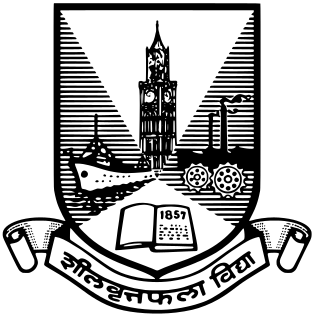
\includegraphics[width=0.2\textwidth]{Images/uom.png}\\[1.5cm]
		\HRule \\[0.4cm]
		{ \huge \textsc \reporttitle}\\[0.4cm] % Title of your document
		\HRule \\[2.5cm]
	\end{center}
	%----------------------------------------------------------------------------------------
	%	AUTHOR SECTION
	%----------------------------------------------------------------------------------------
	\textsc{
		\large A project submitted to\\
		\large Department of Mathematics\\
		\large University of Mumbai\\
		\large by\\[1cm]
		\large Bhoris Dhanjal\\[1em]
		\small Semester III}\\
	
	%----------------------------------------------------------------------------------------
	%	FOOTER & DATE SECTION
	%----------------------------------------------------------------------------------------
	\vfill % Fill the rest of the page with whitespace
	\textbf{
		2024-2025}
			\newpage
		\ 
		\newpage
\end{titlepage}


	\frontmatter
	
	\begin{center}
		

		{\LARGE {\textsc{Certificate}}}\\[2.5cm]
	\end{center}
	\normalsize This is to certify the Semester IV Research Project titled 'Higher Algebraic K-Theory:A simplicial approach' in partial fulfilment of the requirements for the degree of M.Sc. Mathematics  submitted by Mr. Bhoris Dhanjal is approved for submission.
	

	
	\vfill
	
	
	\begin{flushright}
		Dr. Anuradha Garge\\
		(Project Guide)\\[1.5cm]
		Prof. B. S. Desale\\
		(Head of Department)\\
	\end{flushright}
	
	\begin{flushleft}
		Date:
	\end{flushleft}
	\clearpage
	
	\begin{center}
	
	
	{\LARGE {\textsc{Acknowledgements}}}\\[1cm]
\end{center}
TODO NEW
	\clearpage
	\begin{center}
		
		
		{\LARGE {\textsc{Abstract}}}\\[1cm]
	\end{center}
	THINGS TO DO	
\begin{enumerate}
	\item djunctions in simplices
	\item Homotopy in model categories and quillen equivalences 
	\item Kan complexes as fibrant objects
	\item classical model structure on simplical sets
	\item Quillen equivalence between homotopy category of simplicial sets and homotopy category of topological spaces.
	\item Spectral sequences in homological algebra in order to introduce Serre spectral sequences. Needed for proof of Quillen theorem B.
	\item Proof of Quillen theorem B (implies theorem A)
	\item Proofs of Fundamental theorems of higher K theory requires quillen theorem B
	\item fix chapter 2 vector bundles lots of errors
\end{enumerate}
\clearpage
	\tableofcontents
	\mainmatter
	\chapter{Basic homological algebra}
	We begin with some basic prerequisite definitions and results on abelian categories and homological algebra, which provide a foundational framework. These concepts will be used extensively throughout the discussion, forming an assumed background.
	%	
	%	We begin with with basic prerequisites in homological algebra. Introducing the concept of a projective module.
	%	
	%	Unless otherwise specified, all rings considered are assumed to be commutative with unity.
	Abelian categories are essential to understanding homological algebra. It is motivated by the fact that they allow for the use of homological methods in a wide variety of applications and help unify various (co)homology theories. They were first introduced by Grothendieck in his seminal Tohoku paper \cite{grothendieck1957quelques}.
	
	\section{Abelian categories}
	There is a chain of conditions regarding `abelian'-ness of categories, which can be roughly understood as follows.
	\[ \textbf{Abelian} \subseteq \textbf{Pre-Abelian} \subseteq \textbf{Additive} \subseteq \textbf{Ab-Enriched}\]
	
	$\mathbf{Ab}$-Enriched categories \index{Category!$\mathbf{Ab}$-Enriched} (sometimes referred to as pre-additive categories) are categories such that for any objects $A,B \in \mathcal{C}$, the external hom-set $\Hom(A,B)$ has the structure of an abelian group. Furthermore, it has a well-defined notion of composition, which is bilinear due to the monoidal product in $\mathbf{Ab}$, $\Hom(A,B)\otimes \Hom(B,C) =\Hom(A,C)$. We shall be giving definitions of the remaining three types of categories in this section.
	
	We have chosen to omit the precise definitions of the coherence conditions for monoidal and monoidally enriched categories to make this section more accessible. Since these conditions are not explicitly used for computations in this work, the basic background described above will suffice. For a more detailed overview of the definitions of monoidal and monoidally enriched categories, refer to \cite{lane1998categories} for a classical treatment or \cite{riehl2017category} for an excellent modern exposition.
	\begin{example}
		A ring is a single object $\mathrm{Ab}$-Enriched category (in the same sense how a group is realized as a single object category with all arrows invertible).
	\end{example}
	
	
	\begin{proposition}
		In $\mathbf{Ab}$-Enriched categories initial and terminal objects coincide (it is often called the zero object).
	\end{proposition}
	\begin{proof}
		Let $\mathcal{C}$ be an $\mathbf{Ab}$-Enriched category. Note that the Hom-sets between objects have `zero morphisms', i.e. arrows in the Hom-set which behave like the additive identity in the $\mathbf{Ab}$ group induced by it. In particular for $0_{A,B}\in \Hom(A,B)$ we have the property that if $f:B \to C$ then $f\circ 0_{A,B}=0_{A,C}$ and $g: A \to D$ then $0_{A,B}\circ g=0_{D,B}$.
		
		Now suppose $0 \in \mathcal{C}$ is an initial object. There is a unique morphism $0\to 0$ so in its Hom-set its both the additive inverse and the identity. So for any $f:X \to 0$ we can say that by the zero morphism property $f=0$ so also $0$ is a terminal object.
	\end{proof}
	\begin{proposition}
		In $\mathbf{Ab}$-Enriched categories finite coproducts coincide with finite products (i.e. biproducts)\footnote{This also holds over categories enriched over commutative monoids.}.
	\end{proposition}
	\begin{proof}	
		Let $\mathcal{C}$ be an $\mathbf{Ab}$-enriched category and objects $A,B\in \mathcal{C}$ consider the product $A\times B$, which is determined by the following universal property,
		\[\begin{tikzcd}
			& X \\
			A & A\times B & B
			\arrow["{p_1}"', from=2-2, to=2-1]
			\arrow["{p_2}", from=2-2, to=2-3]
			\arrow["u", dashed, from=1-2, to=2-2]
			\arrow["{x_1}"', from=1-2, to=2-1]
			\arrow["{x_2}", from=1-2, to=2-3]
		\end{tikzcd}\]
		Consider $A$ and $B$ in place of $X $ in the diagram. By the universal property we have $q_1: A \to A\times B, q_2: B \to A\times B$
		\[\begin{tikzcd}
			A && B \\
			& {A\times B} \\
			A && B
			\arrow["{p_1}"', from=2-2, to=3-1]
			\arrow["{p_2}", from=2-2, to=3-3]
			\arrow["{q_2}"', from=1-3, to=2-2]
			\arrow["{q_1}"', from=1-1, to=2-2]
			\arrow["{1_A}"', from=1-1, to=3-1]
			\arrow["{1_B}", from=1-3, to=3-3]
		\end{tikzcd}\]
		So $p_1q_1=1_A$ and $p_2q_2=1_B$ also $p_1q_2=p_2q_1=0$.
		
		Now note that $q_1p_1+q_2p_2=1_{A\times B}$ as $p_1(q_1p_1+q_2p_2)=p_1$ and $p_2(q_1p_1+q_2p_2)=p_2$. Claim this $q_1,q_2$ determine a coproduct $A +B$.
		
		We wish to show the following universal property holds for some arbitrary $C \in \mathcal{C}$
		\[\begin{tikzcd}
			A & C & B \\
			& {A\times B} \\
			A && B
			\arrow["{q_1}"', from=1-1, to=2-2]
			\arrow["{q_2}", from=1-3, to=2-2]
			\arrow["{p_1}"', from=2-2, to=3-1]
			\arrow["{p_2}", from=2-2, to=3-3]
			\arrow["{1_B}"', from=1-3, to=3-3]
			\arrow["{1_A}"', from=1-1, to=3-1]
			\arrow["{r_1}", from=1-1, to=1-2]
			\arrow["{r_2}"', from=1-3, to=1-2]
			\arrow["{f}"',dashed, from=2-2, to=1-2]
		\end{tikzcd}\]
		Define $f: A\times B \to C$ as $f=r_1p_1+r_2p_2$. Now $fq_1=r_1$ and $fq_2=r_2$. So if we show uniqueness of $f$ we are done.
		
		Say $f'$ exists \( f':A \times B \to C \), then $(f-f')1_{A \times B}=(f-f')(q_1p_1+q_2p_2)=0$. So $f=f'$.
		
		
	\end{proof}
	
	
	\begin{definition}[Additive category]\index{Category!Additive}
		An $\mathbf{Ab}$-Enriched category which has all finite (co)products (i.e. biproducts since they coincide).
	\end{definition}
	
	\begin{example}
		The category of vector bundles over a topology $X$ is a additive category (but not an abelian category). We will see this in more detail in the following section.
	\end{example}
	Functors between additive categories are called \textit{additive functors}. They	 can be realized as functors which preserve additivity of homomorphisms between modules, $F(f+g)=F(f)+F(g).$
	
	Before proceeding further it is important to think about kernels and cokernels in the categorical sense.
	\begin{definition}[Equalizer]
		An equalizer of pair of parallel morphisms \( f,g:A \to B \) consists of an object \( E \) and a morphism \( e:E \to A \) universal such that \( fe=ge \).
	\end{definition}
	\begin{definition}[Kernel]
			A kernel of a morphism $f:A \to B$ is the pullback along the unique morphism from $0 \to B$, i.e. it is $p: \ker f \to A$, provided initials and pullbacks exist.
			
			\[\begin{tikzcd}
				{\ker f} & 0 \\
				A & B
				\arrow["f", from=2-1, to=2-2]
				\arrow[from=1-2, to=2-2]
				\arrow[from=1-1, to=1-2]
				\arrow["p"',from=1-1, to=2-1]
				\arrow["\lrcorner"{anchor=center, pos=0.125}, draw=none, from=1-1, to=2-2]
			\end{tikzcd}\]
	\end{definition}
	The intuition behind this definition is that alternatively it is seen as an equalizer of a function $f:A \to B$ and the unique zero morphism $0_{A,B}$. The kernel object is the part of the domain that is `going to zero'. \footnote{A minor point to note is that in the case of $\mathbf{Ab}$-Enrichments the `zero' in the Hom-sets isn't a terminal, its Hom-set specific. When you assume a $\mathbf{Ab}$-Enriched category has a initial 0 however this matches up with our intuition.}
		
	A cokernel is simply its categorical dual.
	\begin{definition}[Cokernel]
		A cokernel of a morphism $f:A \to B$ is the pushout along the unique morphism $A \to 1,$ where $1$ is the terminal object.
		\[\begin{tikzcd}
			A & B \\
			1 & {\mathrm{coker} f}
			\arrow["f", from=1-1, to=1-2]
			\arrow[from=1-1, to=2-1]
			\arrow[from=1-2, to=2-2]
			\arrow[from=2-1, to=2-2]
			\arrow["\lrcorner"{anchor=center, pos=0.125, rotate=180}, draw=none, from=2-2, to=1-1]
		\end{tikzcd}\]
	\end{definition}
	
	\begin{definition}[Pre-abelian categories]\index{Category!Pre-abelian}
		An additive category with all morphism having kernels and cokernels is called a pre-abelian category.
	\end{definition}
	The above definition is equivalent to saying a pre-abelian category is a $\mathbf{Ab}$-Enriched category with all finite limits and colimits. 
	
	This is a consequence to the fact that categories have finite limits iff it has finite products and equalizers \cite[Proposition~5.21]{Awodey}, and we know equalizers exist because equalizers of two morphisms is just the kernel of $f-g$.
	
	
	
	
	\begin{definition}[Abelian category]\index{Category!Abelian}
		Pre-abelian categories for which each monomorphism is a kernel and each epimorphism is a cokernel.
	\end{definition}
	Equivalently a category is abelian if its pre-abelian and the map \( \mathrm{coim}(f)\to\mathrm{im}(f) \) is an isomorphism.
	
	
	\begin{example}\label{expreabnotab}
		
		\begin{enumerate}Some non examples are:
			\item The category of Hausdorff topological abelian groups is pre-abelian but not abelian. Since not every morphism which is a monomorphism+epimorphism is necessarily a isomorphism. 
			
			Consider a Hausdorff abelian topological group $G$ with a non discrete topology and consider $G'$ it's discretization. The inclusion map $G' \to G$ is a monomorphism+epimorphism but not isomorphism (bijective continuous group isomorphism). 
			\item The category of torsion free abelian groups $\mathbf{TFAb}$ is pre-abelian but not abelian as the mono $f: \Z \xrightarrow{z\mapsto 2z} \Z $ is not a kernel of some morphism. Say it were and there exists $ A \in \mathbf{TFAb}$ such that $f$ is the kernel to $ g: \Z \to A$, i.e.
			\[\begin{tikzcd}
				Z & 0 \\
				Z & A
				\arrow[from=1-1, to=1-2]
				\arrow["{f(z)=2z}"', from=1-1, to=2-1]
				\arrow["\lrcorner"{anchor=center, pos=0.125}, draw=none, from=1-1, to=2-2]
				\arrow[from=1-2, to=2-2]
				\arrow["g", from=2-1, to=2-2]
			\end{tikzcd}\]
			this implies $1_\Z$ factors through $f$ i.e. $1_\Z =f\circ h$ for some unique $h:\Z \to \Z $ which implies $h(1)=1/2$ which is absurd.
		\end{enumerate}
		
	\end{example}
	\begin{example}Some examples of abelian categories:
		\begin{enumerate}
			\item The category of modules.
			\item Category of representations of a group.
			\item Category of sheaves of abelian groups on some topological space.
			
			%					\begin{definition}[Presheaf]
				%							For a category $\mathcal C$ a presheaf is any functor $F: \mathcal{C}^{\mathrm{op}}\to \mathbf{Sets}$.
				%						\end{definition}
			%					In particular in the case for a topological space $X$ a presheaf of groups (or any algebraic object) on $X$ (in particular the set of the lattice of open sets of $X$ ordered by inclusion) is a some contravariant functor $F$ which sends open sets $U \subseteq X$ to some $F(U)$, it respects inclusions (i.e. there for open sets $V \subseteq V $ is a natural transformation $\rho_{UV}: F(U)\to F(V)$ in the form of a restriction). Furthermore, function composition, unitals and empty sets going to empty sets hold (to make it a category). Note that all these notions of presheaves are really just a special case of the categorical definition where the sheaf of groups is really just a group object in the categorical presheaf.
			%					\begin{definition}[Sheaf of sets on a topology]\label{def:scheaf}
				%							A sheaf of a topology $X$ is a presheaf which satisfies two additional properties, for open sets $U \in X$ and open covers ${U_i}$ of $U$
				%							\begin{enumerate}
					%									\item (Locality) A section, i.e. an element $s \in F(U)$ goes to zero restricted at $U_i$ for all $i$ implies $s=0$.
					%									\item (Gluing) If there is a collection of sections $s_i \in F(U_i)$ such that $s_i|_{U_i \cap U_j}=s_j|_{U_i \cap U_j}$ for all $i,j$ then there is some $s \in F(U)$ such that $s|_{U_i}=s_i$ for all $i$.
					%								\end{enumerate}
				%							
				%							These two conditions can be written is short as just saying we require $F(U)$ to be the equalizer for the following diagram
				%							\[\begin{tikzcd}
					%									{\prod_{i \in I} F(U_i)} && {\prod_{i,j}F(U_i \cap U_j)}
					%									\arrow[shift right=2, from=1-1, to=1-3]
					%									\arrow[shift left=2, from=1-1, to=1-3]
					%								\end{tikzcd}\]
				%						\end{definition}
			%					
			%					The category of sheaves of abelian groups on a topological space form a abelian category. Additivity is natural due to the functorial nature of $F$. A quick proof is due to `sheafification', i.e. the left adjoint to the inclusion functor from sheaves into presheaves. Presheves of abelian groups can be understood to have all the required properties to be an Abelian category due the functorial representation. Now due to the following result \cite[Sec. 6.17]{stacks1} we can extend this notion to the sheaves via sheafification.
		\end{enumerate}
	\end{example}
	

	
	
	
	
	With this definition in mind we will now define a few important constructions we will use often. These are not restricted to abelian categories but we will use them very often in the case of abelian categories, so it is good to see it in action directly with the notion of an abelian category at hand.
	\begin{definition}[Subobject]
		A subobject \( Y \) for some $X \in \mathcal{C}$ is an isomorphism class of monomorphisms $i: Y \to X$. 
		
		\( (i_0:Y_0 \to X) \sim (i_1: Y_1 \to X) \iff i_1=i_2 f \) for an isomorphism \(f:Y_0 \to Y_1 \).
	\end{definition}
	
	
	With slight abuse of notation we refer to $Y \leq X$ as a subobject of $X$ where $Y$ is just a representative of the codomain of a isomorphism class of monomorphisms into $X$. 
	
%	This is clearer when seen through the lens of a slice category. Note that arrows between subobjects of the same $X$ are arrows in the slice category of $X$. So collection of subobjects form a category with a preorder (with inclusion). The reasoning behind such an definition for subobjects is motivated by the fact that we think of generalized elements in $\mathcal{C} $ as being not $X \in \mathrm{Ob}(\mathcal{C}) $ but rather $\Hom_\mathcal{C}(-,X)$.
	
	\begin{definition}[Quotients in abelian categories]
		For $Y \leq X$ in an abelian category we can define $X/Y $ as the cokernel of the monomorphism $Y \to X$. 
	\end{definition}
	
	\begin{definition}[Short exact sequences in abelian categories]
		A sequence of morphisms of the sort \[ 0 \to A \xrightarrow{i} B \xrightarrow{p} C \to 0 \] is refered to as short exact if \( i \) is a monomorphism, \( p \) is an epimorphism and \( \mathrm{im}(i)=\ker(p). \)
	\end{definition}
	
	Note the \( 0 \) object above is the `zero' object which we proved exists.
	
	
	A deep result on abelian categories is the Freyd-Mitchel embedding theorem which helps characterize all small abelian categories in terms of modules.
	
	\begin{theorem}[Freyd-Mitchell]
		Every small abelian category can be faithfully embedded as a full subcategory via an exact functor into $R-$Mod for some ring $R$.
	\end{theorem}
	The proof for the theorem is very extensive and as such is omitted. The canonical reference is Freyd's own book \cite{freyd1964abelian}. A proof sketch summarising Freyd's proof is given in an excellent MathOverflow post by the user Theo Buehler \cite{47762}.
	
%	\begin{proposition}
%		In an abelian category, let the following diagram be a pullback square:
%		\[
%		\begin{tikzcd}
%			P \arrow[r, "i'"] \arrow[d, "p'"'] & A \arrow[d, "p"] \\
%			B \arrow[r, "i"] & C \arrow[ul, phantom, "\lrcorner"{anchor=center, pos=0.125}, very near start]
%		\end{tikzcd}
%		\]
%		Then the kernels of the vertical maps are isomorphic, i.e., \( \ker p' \cong \ker p \).
%	\end{proposition}
%	
%	\begin{proof}
%		The object \( P \) is defined as the pullback \( A \times_C B \).
%		The kernel of \( p: A \to C \) is defined categorically as the pullback of \( p \) along the unique zero morphism \( 0 \to C \):
%		\[
%		\begin{tikzcd}
%			\ker p \arrow[r, "k_0"] \arrow[d, tail, "k_p"'] & 0 \arrow[d, "0_C"] \\
%			A \arrow[r, "p"] & C \arrow[ul, phantom, "\lrcorner"{anchor=center, pos=0.125}, very near start]
%		\end{tikzcd}
%		\]
%		Thus, \( \ker p \cong A \times_C 0 \).
%		
%		Similarly, the kernel of \( p': P \to B \) is the pullback of \( p' \) along the unique zero morphism \( 0 \to B \):
%		\[
%		\begin{tikzcd}
%			\ker p' \arrow[r, "k'_0"] \arrow[d, tail, "k_{p'}"'] & 0 \arrow[d, "0_B"] \\
%			P \arrow[r, "p'"] & B \arrow[ul, phantom, "\lrcorner"{anchor=center, pos=0.125}, very near start]
%		\end{tikzcd}
%		\]
%		Thus, \( \ker p' \cong P \times_B 0 \).
%		
%		Substitute the definition of \( P \) into the expression for \( \ker p' \):
%		\[ \ker p' \cong (A \times_C B) \times_B 0 \]
%		
%		Using the property that limits commute with limits (specifically, pullbacks can be re-associated) in an abelian category:
%		\[ (A \times_C B) \times_B 0 \cong A \times_C (B \times_B 0) \]
%		
%		Now, we evaluate the term \( B \times_B 0 \). This is the pullback defined by the square:
%		\[
%		\begin{tikzcd}
%			B \times_B 0 \arrow[r] \arrow[d] & 0 \arrow[d, "0_B"] \\
%			B \arrow[r, "id_B"] & B \arrow[ul, phantom, "\lrcorner"{anchor=center, pos=0.125}, very near start]
%		\end{tikzcd}
%		\]
%		The universal property implies that any map into the pullback must factor through the zero map into \( B \), hence the pullback object \( B \times_B 0 \) is isomorphic to the zero object \( 0 \).
%		
%		Substituting this result back:
%		\[ \ker p' \cong A \times_C (B \times_B 0) \cong A \times_C 0 \]
%		
%		Since \( A \times_C 0 \) is isomorphic to \( \ker p \), we conclude that:
%		\[ \ker p' \cong \ker p \]
%	\end{proof}
%	
	%	\section{Chain complexes and exact sequences}
	%	In this section we define and prove the essential homological algebra results that we require. For further details refer to \cite{eisenbud2013commutative, weibel_1994}. 
	%	
	%	All of the results below stated for modules over rings apply for abelian categories. The proofs performed via diagram chases are well defined under the Freyd-Mitchel embedding on the full subcategory of the given diagram only.
	%	
	%	\begin{definition}[Chain complex]
		%		A {chain complex} $(A_\bullet, \varphi_\bullet)$ is a collection of modules over a commutative ring and homomorphisms $\varphi_i: A_i \to A_{i-1}$ such that $\varphi_i \varphi_{i+1}=0$.
		%		\[\begin{tikzcd}
			%			\cdots & {A_{i+1}} & {A_i} & {A_{i-1}} & \cdots
			%			\arrow["{\varphi_{i+1}}", from=1-2, to=1-3]
			%			\arrow["{\varphi_i}", from=1-3, to=1-4]
			%			\arrow["{\varphi_{i-1}}", from=1-4, to=1-5]
			%			\arrow["{\varphi_{i+2}}", from=1-1, to=1-2]
			%		\end{tikzcd}\]
		%	\end{definition}
	%	\begin{definition}[Chain (Co)Homology]
		%		The {homology} of the complex at $F_i$ is denoted as its $i^{\mathrm{th}}$ homology defined as follows,
		%		\[ H_iA := \ker \varphi_i/ \mathrm{im} \varphi_{i+1}. \]
		%		Reversing the arrows gives us the analogous definitions for cochain complexes and cohomology.
		%	\end{definition}
	%	
	%	
	%	The homomorphisms are often called {`boundary operators'} or {`differentials'}. This nomenclature is motivated by de Rahm cohomology. Furthermore elements of $\ker \varphi_i$ are called `{cycles}' and elements of $\mathrm{im} \varphi_{i+1}$ are called {boundaries}, this echoes the aphorism `cycles modulo boundaries' often encountered in singular homology.
	%	\begin{definition}[Exact sequence]
		%		A chain complex is said to be {exact} if all its homologies are zero. In particular it is exact at one object if its homology there is zero.
		%	\end{definition}
	%	 An exact sequence of the form \[ 0 \to A \to B \to C \to 0 \]
	%	is referred to as short exact sequence. Note that due to the exactness conditions $A \to B $ is injective and $B \to C$ is surjective.
	%	\begin{proposition}[Splitting lemma]
		%		For a short exact sequence $$0 \to A \xrightarrow{f} B \xrightarrow{g} C \to 0$$ the following are equivalent:
		%		\begin{enumerate}
			%			\item The sequence splits, i.e. $B \cong A \oplus C.$
			%			\item Left split: There is a morphism $h:B \to A $, such that $hf=1_A$.
			%			\item Right split: There is a module morphism $i: C \to B $ such that $gi=1_C$.
			%		\end{enumerate}
		%	\end{proposition}
	%	\begin{proof}
		%		Begin by showing $1$ and $2$ are equivalent then $1$ and $3$.
		%		
		%		
		%	\end{proof}
	%	
	%	\begin{definition}[Chain homotopy]\label{chainhomotopy}
		%		If $\alpha, \beta $ are maps between differential modules $(A, \varphi), (B, \psi )$ then $\alpha $ is homotopically equivalent to $\beta $ if there is a map $h: A \to B $ such that $\alpha - \beta = \psi h+ h \varphi$. If grading is relevant the picture formed is as such, we require a family of maps $h_i: A_i \to B_{i+1}$ \footnote{i.e. It has degree $1$, sometimes the subscript is dropped and just treated as $h$}
		%		\[\begin{tikzcd}
			%			\cdots && {A_i} && {A_{i-1}} && \cdots \\
			%			\\
			%			\cdots && {B_i} && {B_{i-1}} && \cdots
			%			\arrow["{\varphi_i}", from=1-3, to=1-5]
			%			\arrow["{\psi_i}"', from=3-3, to=3-5]
			%			\arrow["{h_{i-1}}"', from=1-5, to=3-3]
			%			\arrow["{\beta_i}"', shift right, from=1-3, to=3-3]
			%			\arrow[from=3-3, to=3-1]
			%			\arrow["{h_i}"', from=1-3, to=3-1]
			%			\arrow["{\alpha_{i-1}}", shift left, from=1-5, to=3-5]
			%			\arrow[from=1-1, to=1-3]
			%			\arrow["{h_{i-2}}"', from=1-7, to=3-5]
			%			\arrow[from=1-5, to=1-7]
			%			\arrow["{\alpha_i}", shift left, from=1-3, to=3-3]
			%			\arrow["{\beta_{i-1}}"', shift right, from=1-5, to=3-5]
			%			\arrow[from=3-5, to=3-7]
			%		\end{tikzcd}\]
		%		The intution behind this particular choice of definition is that the map $\alpha - \beta $ maps all cycles to boundaries which have zero homology. So really $\alpha- \beta$ is null homotopic, as such this relation is an equivalence relation.
		%	\end{definition}
	%	\begin{definition}[Quasi-isomorphism]
		%		A chain map is called a quasi isomorphism if the induced map on the homologies constituents an isomorphism.
		%	\end{definition}
	%	The reason for `quasi' is that the relation is reflexive and transitive but not symmetric. 
	%	\begin{definition}[Homotopy category of chain complexes]
		%		For a given category of chain complexes $\mathbf{Ch}(\mathcal{A})$ we can define $\mathcal{K}(\mathcal{A})$ to be the homotopy category of chain complexes with objects as objects of $\mathbf{Ch}(\mathcal{A})$ and arrows as chain homotopic maps as in Definition\ref{chainhomotopy}.
		%	\end{definition}
	%	
	%	\section{Projective modules}	
	%	The category of finitely generated projective modules is the main object of study in algebraic K-theory. This is largely motivated by a theorem due to Swan's which we will prove in the next project.
	%	
	%	Recall the definition of a free module.
	%	\begin{definition}[Free module of rank $n$]
		%	A module over a ring $A$ is said to be free with rank $n$ if it is isomorphism to a module of the form $A^n$.
		%	\end{definition}In particular this means that there exists a linearly independent spanning set of the module with $n$ elements.
	%	
	%	Note homomorphisms from free modules to other modules are determined by the image of their generators.
	%	, i.e. free objects are left adjoints to forgetful functors. \footnote{This holds in free monoids $\mathrm{Hom}_\mathbf{Mon}(F(X), M) \cong \mathrm{Hom}_\mathbf{Sets} (X, U(M))$ where $F(X)$ denotes the free monoid generated by elements from the set $X$ and $U(M)$ is the underlying set of a monoid $M$, refer to \cite[p. ~208]{Awodey} }
	%	\begin{definition}[Projective module]
		%		A module $P$ is said to be {projective} if it satisfies the following lifting property, every morphism from $P$ to $N$ factors through an epimorphism into $N$. Note that the lift need not be unique.
		%		\[\begin{tikzcd}
			%			&& M \\
			%			\\
			%			P && N
			%			\arrow[two heads, from=1-3, to=3-3]
			%			\arrow[from=3-1, to=3-3]
			%			\arrow[dashed, from=3-1, to=1-3]
			%		\end{tikzcd}\]
		%	\end{definition}
	%	
	%	
	%	
	%	
	%	\begin{proposition}[Equivalent definitions of projectivity]\label{projtfae}
		%		The following are equivalent,
		%		\begin{enumerate}
			%			\item $P$ is projective.
			%			\item For all epimorphisms between $M\twoheadrightarrow N$, the induced map $\Hom(P,g):\mathrm{Hom}(P,M) \to \mathrm{Hom}(P,N)$ sending $f \mapsto g \circ f$ for $g:M \to N$ and $f:P \to M$ is an epimorphism.
			%			\item For some epimorphism from a free module $F$ to $P$, $\mathrm{Hom}(P,F) \to \mathrm{Hom}(P,P)$ is an epimorphism.
			%			\item There exists $Q$ s.t. $P \oplus Q$ is free.
			%			\item Short exact sequences of the form $0 \to A \to B \to P \to 0$ split, i.e. isomorphic to another short exact where middle term is $A \oplus P$. \footnote{In general any epimorphisms into projective objects split (i.e. have an inverse).}
			%		\end{enumerate}
		%	\end{proposition}
	%	
	%	\begin{proof}
		%		$1 \iff 2$ is restatement of definitions.
		%		
		%		$2 \implies 3$ is also just substitution.
		%		
		%		$3 \implies 4$ consider a map in the preimage of identity in $\Hom(P,P)$ which is a splitting (inverse) of the epimorphism $F$ into $P$,
		%		\[\begin{tikzcd}
			%			& P \\
			%			\\
			%			F && P
			%			\arrow["g", shift left=3, two heads, from=3-1, to=3-3]
			%			\arrow[""{name=0, anchor=center, inner sep=0}, "f"', from=1-2, to=3-1]
			%			\arrow[""{name=1, anchor=center, inner sep=0}, "{\mathrm{Id}_P=g \circ f}", dashed, two heads, from=1-2, to=3-3]
			%			\arrow[shorten <=6pt, shorten >=6pt, Rightarrow, from=0, to=1]
			%		\end{tikzcd}\]
		%		Now we have a short exact sequence $0 \to \ker g \to F \to P \to 0$, and also $f\circ g $ is idempotent so it naturally admits a decomposition $F = \image(f \circ g) \oplus \kernel (f \circ g)$\footnote{For some idempotent $e$, $1-e$ is also an idempotent and images under these two mappings decompose any module, furthermore image of $1-e$ is just kernel of $e$}=$\image (g) \oplus \kernel (g)$ the first by the 1st isomorphism theorem and the second by $f $ being a mono.
		%		
		%		$4 \implies 2$ simply as $\Hom (P \oplus Q,-) = \Hom(P,-) \oplus \Hom(Q,-)$
		%		
		%		$1 \iff 5$ To show that $0\to A \to B \xrightarrow{\varphi} P$ splits we need to show that there exists a $\psi: P \to B$ such that $\varphi \circ \psi = 1_P$. This is just obtained by the definition of $P$ being projective.
		%		\[\begin{tikzcd}
			%			&& M \\
			%			\\
			%			P && P
			%			\arrow["\varphi", from=1-3, to=3-3]
			%			\arrow["\psi", dashed, from=3-1, to=1-3]
			%			\arrow["{=}", from=3-1, to=3-3]
			%		\end{tikzcd}\]
		%		
		%	\end{proof}
	%	\begin{lemma}[Free modules are projective]
		%	\end{lemma}
	%	\begin{proof}
		%		Consider the preimages of images of basis of $P$ in $N$, that lie in $M$. Then map basis elements from $P$ into these preimages.
		%	\end{proof}
	%	\begin{example}[Projective modules are not always free]
		%		Let $R,S $ be two non-trivial commutative rings with unity, consider $R \oplus S$ as a (free) module over itself. Consider $R \oplus \{0\}$ as a submodule of $R \oplus S$, it is projective as it is a direct summand of $R \oplus S$. However, it cannot be free as $(R \oplus \{0\})^n \not \cong R\oplus S $ for any $n$.
		%	\end{example}
	%	
	%	\begin{theorem}\label{a2}Projective finitely generated modules over local rings are free.
		%	\end{theorem}
	%	\begin{proof}
		%		Pick a minimal set of generators and see its residue classes in $M/\mathfrak{m}M$ as the basis of it as a vector space over $R/\mathfrak{m}$.
		%		
		%		Now as for some free module $F, F=\varphi(M)\oplus K$ for some $K$ and some homomorphism $\varphi: M \to F$, (by definition of projective module), 	we get \[ M/\mathfrak{m}M \cong 	F/\mathfrak{m}F = (R/\mathfrak{m})^n\cong R^n\otimes R/\mathfrak{m} \cong F \otimes R/\mathfrak{m} \cong (\varphi(M)\oplus K) \otimes R/\mathfrak{m}\]
		%		
		%		Finally we get $M/\mathfrak{m}M \cong M/\mathfrak{m}M \oplus K/\mathfrak{m}K\implies K=\mathfrak{m}K \implies K=0$ by Nakayamas lemma.
		%	\end{proof}
	%	This holds for not necessarily finitely generated modules too refer to \cite[Theorem~2.5]{matsumura_1987}	.
	%	
	%	Using the convention of \cite{lam1999lectures} we define the rank of a projective module as such.
	%	\begin{definition}[Rank of a finitely generated projective module]\label{def:rankproj}
		%		For any finitely generated projective module $P$ over commutative ring $A$ the localization $P_\mathfrak{p} =P \otimes_A A_\mathfrak{p}$ is also a finitely generated $A_\mathfrak{p}$ module, but $P_\mathfrak{p}$ being local is free by Theorem \ref{a2}. So the local rank of $P$ is defined as the rank of the free $P_\mathfrak{p} $ module.
		%		
		%		This induces a map $\phi: \mathrm{Spec}(A) \to \Z $ sending each $\mathfrak{p}$ to the local rank of $P$. If $\phi $ is constant and the rank of $P$ is the same for all localizations then we refer to that as the rank of $P$.
		%	\end{definition}
	%	
	%		\begin{proposition} If $M$ is a finitely presented module over a Noetherian ring $R$ (prime ideals fin gen) then TFAE
		%				
		%				
		%				\begin{enumerate}
			%						\item $M$ is projective.
			%						\item $M$ localized at maximal ideals is free.
			%						\item A finite set of elements $\{x_i\}^n$ in $R$ generate $R$ such that $M[x_i^{-1}]$ is free over $R[x_i^{-1}]$.
			%					\end{enumerate}		
		%			\end{proposition}
	%		This proceeds just from the previous result.
	%		\begin{lemma}\label{suboffgisfgnoet}
		%				$A$ is Noetherian iff all submodules of finitely generated $A$ modules are finitely generated.
		%			\end{lemma}
	%	\begin{proposition}\label{submodoffreemodisfreepid}
		%		For a principal ideal domain $A$ a submodule $M$ of a free module of finite rank say $A^n $ is free, and the submodule has rank $\leq n$.
		%	\end{proposition}
	%	\begin{proof}
		%		We prove this by induction on $n$. When $n=0$ there is nothing to prove. For $n=1$ due to the fact that $A$ is a principal ideal domain the submodules of $A$ (ideals) are one generated i.e. they are rank 1 free modules of $A$.
		%		
		%		Proceed via induction. Now consider the case when $n=k$. 
		%		
		%		Let $M \subset A^k$ be non zero. Consider the componentwise projection maps $p_i: A^{k} \to A$ for each $i$. Then $\pi_i(M) \neq \{0\}$ for some $i$. Therefore $p_i(M)$ is a non-zero ideal in $A$, i.e. free with rank 1. Also, $\ker p_i \cap M$ is a submodule of $\ker p_i$ which is itself free of rank $n-1$. Therefore rank of $\ker p_i \cap M$ is $\leq n - 1$. Let $a$ be a generator for $p_i(M)$ consider some preimage of it as $a_p$.
		%		
		%		Now $M = \ker p_i \cap M \oplus \langle a_p \rangle$. If $\{a_1, a_2, \cdots a_m\}$ is a basis of $\ker p_i \cap M$, then $\{a_1, a_2, \cdots a_m, a_p \}$ is a basis of $M$. Hence rank of $M$ equals $m + 1 \leq n$. 
		%		
		%	\end{proof}
	%	
	%	\begin{proposition}\label{projfgpidfree}
		%		Projective finitely generated modules over principal ideal domains are free.
		%	\end{proposition}
	%	\begin{proof}
		%		Every finitely generated projective module $P$ is a direct summand of a free module $F$ meaning it is a submodule of $F$ and by Proposition \ref{submodoffreemodisfreepid} it is free.
		%	\end{proof}
	%	
	%	\begin{definition}[Stably isomorphic]\label{stabiso}
		%		Two $A-$modules $M,N$ are said to be stably isomorphic if there exists $r$ such that $M \oplus A^r \cong M \oplus A^r$.
		%	\end{definition}
	%	\begin{definition}[Stably free module]\label{stabfree}
		%		An $A$ module $M$ is stably free if there exists a finitely generated free module $F$ such that $M \oplus F$ is free, i.e. if $M$ is stably isomorphic to a finitely generated free $A$ module.
		%	\end{definition}
	%	
	%			Note If $R$ is local and $M$ is fin-gen projective module then $M$ is free, this is a consequence of Nakayama. As $M \oplus Q = R$ so if $R$ has maximal ideal $\mathfrak{m}$ then $M/\mathfrak{m}M$ is a vector space	over the field $R/\mathfrak{m}R$ and its basis lifts to minimal set of generators of $M$, consider $N=M/\sum R m_i$ and so $ N/ IN=M/(IM+\sum_i R m_i)=M/M=0\implies N=IN$ then apply typical Nakayama to get $N=0
	%			\implies M= \sum_i R m_i$, for $I$ an ideal inside the Jacobson radical of $R$
	%			
	%			So now to prove $1 \iff 2 $ consider a finitely presented module localized over 
	%			
	%			If $M,N$ finitely presented over $R$ and their localizations are isomorphic then theres some element of $f\in R-P$ such that $M[f^{-1}] \cong N[f^{-1}]$
	%	
	%	
	%	\section{Long exact sequence of homologies}
	%	
	%	Consider $(A,\varphi),(B,\psi),(C,\chi)$ to be chain complexes we can define a short exact sequence of complexes as \[ 0 \to A \xrightarrow{\alpha} B \xrightarrow{\beta} C \to 0 \]
	%	For $\alpha, \beta $ maps of complexes as discussed above, and $\beta \alpha=0$, if for all $i$ the underlying sequence of modules is exact\[ 0 \to A_i \xrightarrow{\alpha_i } B_i \xrightarrow{\beta_i } C_i \to 0\]
	%	
	%	These maps also induce maps on the homologies $\alpha_i: H_i A \to H_i B, \beta_i: H_i B \to H_i C$. Furthermore there is a natural map \[ 	\delta_i : H_i C \to H_{i-1}A	 \] which is called the \textbf{connecting homomorphism}
	%	
	%	Before seeing how to construct this $\delta $ it is useful to have a complete picture of the data in front of us. This can be seen below,
	%	\[\begin{tikzcd}
		%		& \vdots & \vdots & \vdots \\
		%		0 & {A_i} & {B_i} & {C_i} & 0 \\
		%		0 & {A_{i-1}} & {B_{i-1}} & {C_{i-1}} & 0 \\
		%		0 & {A_{i-2}} & {B_{i-2}} & {C_{i-2}} & 0 \\
		%		& \vdots & \vdots & \vdots
		%		\arrow[from=2-1, to=2-2]
		%		\arrow["{\alpha_i}", from=2-2, to=2-3]
		%		\arrow["{\beta_i}", from=2-3, to=2-4]
		%		\arrow[from=2-4, to=2-5]
		%		\arrow[from=3-1, to=3-2]
		%		\arrow[from=4-1, to=4-2]
		%		\arrow["{\alpha_{i-1}}", from=3-2, to=3-3]
		%		\arrow["{\beta_{i-1}}", from=3-3, to=3-4]
		%		\arrow[from=3-4, to=3-5]
		%		\arrow["{\alpha_{i-2}}", from=4-2, to=4-3]
		%		\arrow["{\beta_{i-2}}", from=4-3, to=4-4]
		%		\arrow[from=4-4, to=4-5]
		%		\arrow["{\varphi_i}"', from=2-2, to=3-2]
		%		\arrow["{\varphi_{i-1}}"', from=3-2, to=4-2]
		%		\arrow[from=4-2, to=5-2]
		%		\arrow[from=1-2, to=2-2]
		%		\arrow[from=1-3, to=2-3]
		%		\arrow[from=1-4, to=2-4]
		%		\arrow["{\psi_i}"', from=2-3, to=3-3]
		%		\arrow["{\chi_i}"', from=2-4, to=3-4]
		%		\arrow["{\psi_{i-1}}"', from=3-3, to=4-3]
		%		\arrow["{\chi_{i-1}}"', from=3-4, to=4-4]
		%		\arrow[from=4-3, to=5-3]
		%		\arrow[from=4-4, to=5-4]
		%	\end{tikzcd}\]
	%	We construct via a diagram chase. Suppose $h \in H_i C= \ker \chi_i / \image \chi_{i+1} $ pick a cycle $x\in \ker \chi_i$. As $\beta_i $ is surjective we know there exists $y \in B_i$ s.t. $\beta_i(y)=x $. Now also by the fact that $x\in \ker \chi_i$ and that we have maps between chain complexes so the squares commute. We have that $\beta_{i-1}(\psi_{i}(y))=\chi_i(\beta_i(y))=\chi_i(x)=0$.
	%	
	%	Now there is some $z \in A_{i-1}$ such that $\alpha_{i-1}(z)=\psi_i(y)$ (this is due to exactness of $i-1$ sequence hence the quotient isomorphism and the above condition).
	%	
	%	As $\alpha_{i-2}$ is a monomorphism $\alpha_{i-2} \varphi_{i-1}(z)=\psi_{i-1}\alpha_{i-1}(z)=\psi_{i-1}\psi_{i}(y)=0$ so $z\in \ker \alpha_{i-1}$. Just define $\delta_i(h) $ to be the image of $z$ in $H_{i-1}A$.
	%	
	%	The above definition is well defined as it is independent of the choice of lift $x$. Pick any other lift say $x'$ now $\beta_i(x-x')=x-x=0$. So it has a preimage in $A_i$ and can be given as an embedding from $A_i \to B_i$ so $x-x' \in A_i$. $\phi_i(x-x')=\psi_i x - \psi_i x'$ which implies their images in $H_{i-1}A$ are homotopic.
	%	
	%	The fact that $\delta_i $ is a group homomorphism is simply via linearity.
	%	
	%	\begin{proposition}[Induced long exact sequence of homology]
		%		For a given short exact sequence 
		%		\[ 0 \to A \xrightarrow{\alpha } B \xrightarrow{\beta } C \to 0\]
		%		of chain complexes $(A, \varphi), (B, \psi), (C, \chi)$, then the connecting homomorphism $\delta_i: H_iC \to H_{i-1}A$ induces the following long exact sequence of homologies
		%		\[\begin{tikzcd}
			%			& \cdots & {H_iC} \\
			%			{H_{i-1}A} & {H_{i-1}B} & {H_{i-1}C} \\
			%			{H_{i-2}A} & \cdots
			%			\arrow[from=1-2, to=1-3]
			%			\arrow[from=2-1, to=2-2]
			%			\arrow[from=2-2, to=2-3]
			%			\arrow["{\delta_i}"{description}, from=1-3, to=2-1]
			%			\arrow["{\delta_{i-1}}"{description}, from=2-3, to=3-1]
			%			\arrow[from=3-1, to=3-2]
			%		\end{tikzcd}\]
		%		
		%		Furthermore if the chain complexes are differential modules the following triangle commutes,
		%		\[\begin{tikzcd}
			%			HA && HB \\
			%			& HC
			%			\arrow["\alpha", from=1-1, to=1-3]
			%			\arrow["\beta", from=1-3, to=2-2]
			%			\arrow["\delta", from=2-2, to=1-1]
			%		\end{tikzcd}\]
		%		
		%	\end{proposition}
	%	
	%	\begin{lemma}[Snake lemma]
		%		\[\begin{tikzcd}
			%			& A & B & C & 0 \\
			%			0 & {A'} & {B'} & {C'}
			%			\arrow[from=1-2, to=1-3]
			%			\arrow[from=1-3, to=1-4]
			%			\arrow[from=1-4, to=1-5]
			%			\arrow[from=2-1, to=2-2]
			%			\arrow[from=2-2, to=2-3]
			%			\arrow[from=2-3, to=2-4]
			%			\arrow["\alpha", from=1-2, to=2-2]
			%			\arrow["\beta", from=1-3, to=2-3]
			%			\arrow["\gamma", from=1-4, to=2-4]
			%		\end{tikzcd}\]
		%		The above commutative diagram induces a exact sequence \[ \ker \alpha \to \ker \beta \to \ker \gamma \to \mathrm{coker}\alpha \to \mathrm{coker}\beta \to \mathrm{coker}\gamma \]
		%	\end{lemma}
	%	\begin{proof}
		%		The map $\ker \gamma \to \mathrm{coker} \alpha $ is given by the connecting homomorphism.
		%	\end{proof}
	%	
	%	\begin{lemma}[5-lemma]
		%		If we have a commutative diagram as such,
		%		\[\begin{tikzcd}
			%			A & B & C & D & E \\
			%			{A'} & {B'} & {C'} & {D'} & {E'}
			%			\arrow[from=1-1, to=1-2]
			%			\arrow["\alpha"', from=1-1, to=2-1]
			%			\arrow[from=1-2, to=1-3]
			%			\arrow["\beta"', from=1-2, to=2-2]
			%			\arrow[from=1-3, to=1-4]
			%			\arrow["\gamma"', from=1-3, to=2-3]
			%			\arrow[from=1-4, to=1-5]
			%			\arrow["\delta"', from=1-4, to=2-4]
			%			\arrow["\epsilon"', from=1-5, to=2-5]
			%			\arrow[from=2-1, to=2-2]
			%			\arrow[from=2-2, to=2-3]
			%			\arrow[from=2-3, to=2-4]
			%			\arrow[from=2-4, to=2-5]
			%		\end{tikzcd}\]
		%		and if $\beta, \delta $ are isomorphisms with $\alpha $ epimorphism and $\epsilon $ a monomorphism implies that $\gamma $ is an isomorphism.
		%	\end{lemma}
	%	
%	\section{Resolutions}
%	Let $\mathcal{A}$ be an abelian category.
%	\begin{definition}\label{defresolution}[Left resolution]
%		Given $M \in \mathcal{A}$ its {left resolution} is given by the data of a exact sequence $(A_\bullet, \varphi_\bullet)$ into $M$ as such,
%		\[ 	\dots \to A_1	\to A_0 \xrightarrow{\epsilon} M \to 0 \]
%		where $\epsilon $ is called the {augmentation map}, if the exact sequence is free its a free resolution and such for projective. 
%	\end{definition}
%	
%	
%	If we have a cochain complex instead it forms a {right resolution} and if its elements are injective we call them injective resolutions.
%	
%	We cover a result about stably free modules. We will revisit this in greater detail in further sections.
%	\begin{lemma}\label{stabfreefinfreeres}
%		A projective module is stably free iff if has a finite free resolution.
%	\end{lemma}
%	\begin{proof}
%		Say $M \in A-$Mod and is projective. Then $M$ is stably free implies $M \oplus A^n \cong A^m$ for some $n,m$. So $M$ has a finite free resolution given by
%		\[ 0 \to A^n \to A^m \to M \to 0 \]
%		Conversely if $M$ is a projective module with a finite free resolution.
%		\[ 0 \to F_n \to \cdots \to F_0 \to M \to 0 \] for $F_i$ free modules over $A$.
%		
%		We proceed via induction on $n$. If $n=0$ then we are done as simply $M$ is free.
%		Let $M_1$ denote the kernel of $F_0 \to M$. Since $M$ is projective, $F_0 = M \oplus M_1$. Now $M_1$ is projective and has a free resolution of length $< n$.
%		
%		Thus, by the induction hypothesis, $M_1 \oplus F$ is free for some finite free module $F$, i.e. $M_1$ is stably free.
%		
%		Consequently $F_0 \oplus F$ is trivially finitely free and so $F_0\oplus F \cong (M\oplus M_1) \oplus F \cong M \oplus (M_1 \oplus F)$ is finite free, i.e. $M$ is stably free.
%	\end{proof}
	
%	\begin{theorem}\label{finitefreeresolutionninelemma}
%		Given a short exact sequence $0 \to A \to B \to C\to 0$. If any two of these objects have a finite free resolution then so does the third.
%	\end{theorem}
%	
%	\begin{proposition}[Horseshoe lemma]
%		If there is a short exact sequence,
%		\[ 0 \to M \to N \to P \to 0 \]
%		and both $M,P$ have a projective resolutions $A, C$ 
%		\[\begin{tikzcd}
%			&&& 0 \\
%			\cdots & {A_1} & {A_0} & M & 0 \\
%			&&& N \\
%			\cdots & {C_1} & {C_0} & P & 0 \\
%			&&& 0
%			\arrow[from=2-4, to=2-5]
%			\arrow[from=1-4, to=2-4]
%			\arrow[from=2-4, to=3-4]
%			\arrow[from=3-4, to=4-4]
%			\arrow[from=4-4, to=4-5]
%			\arrow[from=4-4, to=5-4]
%			\arrow[ from=4-3, to=4-4]
%			\arrow[ from=2-3, to=2-4]
%			\arrow[from=2-1, to=2-2]
%			\arrow[from=2-2, to=2-3]
%			\arrow[from=4-1, to=4-2]
%			\arrow[from=4-2, to=4-3]
%		\end{tikzcd}\]
%		as below then $N$ also has a projective resolution $B$ which forms a short exact sequence. Also the sequence splits due to $C_i$ being projective so $B_i=A_i \oplus C_i$.
%	\end{proposition}
%	\begin{proof}
%		First note $\epsilon_P: C_0 \to P$ lifts due to projectivity to $C_0 \to N$ also $A_0\to N$ via composition so simply define $B_0 = A_0 \oplus C_0$. This is an epimorphism evidently via diagram chase. Also is projective as direct sum of projectives is projective. Now consider direct sum of kernel of $A_0 \to M, B_0 \to N, C_0 \to P$ and construct the direct sum again to get $F_1$.	Now we get a $3\times 3$. Exactness is due to the Snake lemma
%	\end{proof}
%	
%	A standard example of a resolution is the Koszkul complex.
%	\begin{definition}[Tensor algebra]
%		For a $R$-Module $M$ and $T^n M = \otimes^n M$ the tensor algebra is defined to be \[ T(M)=\oplus_{n=0}^\infty T^n M \]
%	\end{definition}
%	
%	
%	
%	\begin{definition}[Exterior algebra and wedge product]
%		For an $R$-Module $M$. Consider the Tensor algebra $T(M)=\oplus_n \otimes^n M	$. Consider the ideal $I$ spanned by elements $v \otimes v$ for $v \in T(M)$.
%		
%		The quotient of $T(V)/I := \Lambda(M) $ is called the exterior algebra and its product the wedge product.	It is universal with respect to multilinear alternating maps.
%		
%		For $v \Lambda^nM, w \in \Lambda^m M$ multiplication is defined as such,
%		\[ v \Lambda w = (-1)^{nm} w \Lambda v\]
%	\end{definition}
%	
%	
%	\begin{example}[Koszul complex]
%		For a $R$-module $M$ there is an associated chain complex of $n^\textbf{th}$ exterior algebras
%		\[ \Lambda^n M \to \Lambda^{n-1} M \to \dots \to \Lambda^0 M \cong M \]
%	\end{example}
%	
%	
%	
%	%	Consider $n$- linear maps for some map between $R$-Modules $M,P$. Repeated application of the tensor product still provides us with universal such module, $M^n \to \otimes_{i=1}^n M$.
%	%		
%	%		Also a map is called $n$-alternating if it vanishes when two of the arguments are the same. This also implies that sign changes when the arguments are interchanged. Also for a permutation the sign change changes to the sign of the permutation. Now when we require a notion of a universal $n$-linear alternating map we arrive to the definition of a wedge product.
%	%		
%	%		In particular for a specific $n$. There is a universal alternating $n$-linear map sending $M \to \Lambda^n M$. If $M$ is finitely generated by $r$ elements then $\Lambda M^n$ is a free module of rank $\binom{r}{n}$.
%	%		
%	%		
%	
%	
%	
%	%	\subsection{Moore complex and normalized chain complex}
%	%	
%	%	Prior to discussing the Dold-Kan correspondence proper there is the question of constructing a complex from a simplicial object. There are three different ways to approach this all of which end up being closely related to each other.
%	%	
%	%	The first is the Moore complex.
%	%	\begin{definition}[Moore complex]
%		%		For a simplical abelian group $A_.$ associate a complex $A_\bullet$ whose $n^\mathrm{th}$ component is $A_n \in A_.$ with boundary maps $\partial:A_n \to A_{n-1}$ given by alternating sum of face maps $\sum_i^n (-1)^i d_i$
%		%	\end{definition}
%	%	
%	%	Once again the singular chain complex is the Moore complex of the simplicial abelian group associated to the singular complex of a topological space.
%	%	
%	%	
%	%	The second is a subcomplex of the Moore complex $DA_\bullet$ wherein the components are degenerate simplicies (i.e. it is in the image of some degeneracy map).	The simplicial identities allow the construction to be a well defined complex.
%	%	
%	%	The third is the Normalized chain complex of a simplicial abelian group $NA_\bullet$ where the $n^\text{th}$ component is the subobject of $A_n$ which vanishes under face maps with differentials being only $(-1)^n d_n$ once again well definedness is due to the simplicial identities.
%	%	\begin{definition}[Normalized chain complex]
%		%		$A \in \mathbf{sAb}$, the complex $NA_\bullet $ is defined as 
%		%		\[ NA_n = \bigcap_{i=0}^{n-1} \ker(d_i) \subset A_n\]
%		%		With differentials as $\partial: NA_n \to NA_{n-1}$ defined as $(-1)^n d_n$ which forms a chain complex due to the simplicial identity $d_{n-1}d_n=d_{n-1}d_{n-1}.$
%		%	\end{definition}
%	%	
%	%	As it turns out the normalized chain complex and the subcomplex of the Moore complex we defined are isomorphic as chain complexes.
%	%	
%	%	\begin{theorem}
%		%		content
%		%	\end{theorem}
%	%	\subsection{Simplicialization functor}
%	%	We have already seen some motivation for 
%	%	
%	%	
%	%	\subsection{Dold-Kan Correspondence for abelian groups}
%	%	
%	%	
%	%	
%	%	\begin{theorem}[Dold-Kan]
%		%		There is a equivalence of categories $$N:\mathbf{sAb}\rightleftarrows \mathbf{Ch}_+: \Gamma$$ where $N$ denotes the normalized chain complex functor and $\Gamma$ the simplicalization functor.
%		%	\end{theorem}
%	%	\begin{proof}
%		%		We need to show a natural transformation between $\Gamma N A \cong A$ and $N \Gamma C \cong C$
%		%	\end{proof}
%	%	Selecta Mathematica (2021) 27:14
%	%	https://doi.org/10.1007/s00029-021-00618-5	
%	%	\subsection{Some applications of Dold-Kan}
%	%	https://mathoverflow.net/questions/437382/applications-of-the-dold-kan-correspondence
%	%	Construct Eilenberg Maclane spaces
%	%	
%	%	Derived functors of non additive functors
%	\section{Category of chain complexes}
%	
%	The discussion in this section follows \cite{weibel_1994}.
%	
%	\begin{definition}[Category of chain complexes]
%		For an abelian category $\mathcal{A}$, the collection of chain complexes in $\mathcal{A}$ with morphisms as chain maps form a category often denoted as $\mathbf{Ch}(\mathcal{A})$. It is again an abelian category.
%	\end{definition}
%	Interestingly enough the category of chain complexes is in fact also a closed monoidal category.
%	
%	\begin{definition}[Tensor product of chain complexes]\label{tensorchain}
%		For $A, B \in \mathbf{Ch}(\mathcal{A})$ define $A \otimes B$ component wise as, \[ (A \otimes B)_n = \bigoplus_{i+j=n} A_i \otimes B_j.\] With the differential as $ \varphi_n(a,b)=(\varphi_Aa\otimes b)+(-1)^{\mathrm{deg}(a)}(a \otimes \varphi_B b)$
%	\end{definition}
%	This of course only makes sense provided $\mathcal{A}$ admits tensors. When discussing homological algebra in the context of $R-$Mod this distinction need not be made.
%	
%	The mysterious sign rule (often referred to as the Koszul sign rule') can be motivated in one of many different ways. 
%	
%	The most important is that the monoidal product arises naturally when we consider the problem of reducing the double complex we obtain by tensoring piecewise (i.e. finding the total complex but we will see this later).
%	
%	Perhaps another interesting way to motivate it with the notion of a `Day convolution'. The following treatment is due to a MathOverflow answer by Alexander Campbell \cite{359316}.
%	
%	A Day convolution can be realized as a categorification of typical convolution product. We do not delve into this in any more detail.
%	%	\begin{definition}[Promonoidal category]
%		%		content
%		%	\end{definition}
%	%	\begin{definition}[Profunctor]
%		%		content
%		%	\end{definition}
%	%	\begin{definition}[Day Convolution as a coend]
%		%		content...
%		%	\end{definition}
%	%	Finally it makes sense to consider that there is a promonoidal structure on $\mathbf{Ch}(\mathcal{A})$.
%	%	
%	\begin{definition}[Internal hom of chain complexes]\label{internalchain}
%		For $A,B \in \mathbf{Ch}(\mathcal{A})$ we define an internal hom object as a chain complex with the following components
%		\[ [A,B]_n=\prod_i \mathrm{Hom}(A_i,Y_{i+n})\]
%		with differentials for $x \in [A,B]_n$
%		\[ \varphi_n x= \varphi_B x-(-1)^n x \varphi_A \]
%	\end{definition}
%	The above two definitions characterize $\mathbf{Ch}(\mathcal{A})$ as a closed monoidal category. 
%	\begin{definition}[Unital tensor]\label{chunittensor}
%		The unital tensor is considered as the unital tensor of $\mathcal{A}$ say $1_\mathcal{A}$ understood as a chain complex $\cdots \to 0\to0 \to 0 \to 1_\mathcal{A}$ (i.e. a chain complex concentrated at 0). In particular when $\mathcal{A}=R-$Mod the unital tensor is just $R$.
%	\end{definition}
%	
%	
%	
%	\section{Homotopy category of a chain complex}
%	We don't immediately use the contents of this section. However, before diving straight into the abstract homotopy theory in the further chapters it is a good idea to first work with the more natural setting of category of chain complexes.
%	
%	The notion of a homotopy category and derived category (i.e. localisation at weak equivalences) will all be made more clear in the further chapters where we will realize the notion of a chain complex as a ``abelianised'' simplicial set\footnote{This is the Dold-Kan correspondence.}.
%	
%	\begin{definition}[Quasi isomorphism]
%		A chain map is called a quasi isomorphism if the induced map on the homologies constituents an isomorphism.
%	\end{definition}
%	The reason for `quasi' is that the relation is reflexive and transitive but not symmetric. 
%	\begin{definition}[Chain homotopy]\label{chainhomotopy}
%		If $\alpha, \beta $ are maps between differential modules $(A, \varphi), (B, \psi )$ then $\alpha $ is homotopically equivalent to $\beta $ if there is a map $h: A \to B $ such that $\alpha - \beta = \psi h+ h \varphi$. If grading is relevant the picture formed is as such, we require a family of maps $h_i: A_i \to B_{i+1}$ \footnote{i.e. It has degree $1$, sometimes the subscript is dropped and just treated as $h$}.
%		\[\begin{tikzcd}
%			\cdots && {A_i} && {A_{i-1}} && \cdots \\
%			\\
%			\cdots && {B_i} && {B_{i-1}} && \cdots
%			\arrow["{\varphi_i}", from=1-3, to=1-5]
%			\arrow["{\psi_i}"', from=3-3, to=3-5]
%			\arrow["{h_{i-1}}"', from=1-5, to=3-3]
%			\arrow["{\beta_i}"', shift right, from=1-3, to=3-3]
%			\arrow[from=3-3, to=3-1]
%			\arrow["{h_i}"', from=1-3, to=3-1]
%			\arrow["{\alpha_{i-1}}", shift left, from=1-5, to=3-5]
%			\arrow[from=1-1, to=1-3]
%			\arrow["{h_{i-2}}"', from=1-7, to=3-5]
%			\arrow[from=1-5, to=1-7]
%			\arrow["{\alpha_i}", shift left, from=1-3, to=3-3]
%			\arrow["{\beta_{i-1}}"', shift right, from=1-5, to=3-5]
%			\arrow[from=3-5, to=3-7]
%		\end{tikzcd}\]
%		The intution behind this particular choice of definition is that the map $\alpha - \beta $ maps all cycles to boundaries which have zero homology. So really $\alpha- \beta$ is null homotopic, as such this relation is an equivalence relation.
%	\end{definition}
%	
%	\begin{definition}[Homotopy category of chain complexes]
%		For a given category of chain complexes $\mathbf{Ch}(\mathcal{A})$ we can define $\mathcal{K}(\mathcal{A})$ to be the homotopy category of chain complexes with objects as objects of $\mathbf{Ch}(\mathcal{A})$ and arrows as chain homotopic maps.
%	\end{definition}
%	
%	Compare this with the notion of the naive homotopy category of topological spaces $\mathbf{hTop}$ in which objects are topological spaces and maps are homotopy classes of maps between spaces.
%	
%	
%		\section{Cones, cylinders and homotopy cofiber (Puppe) sequences}
%		
%		
%		The notion of mapping cones and cylinders are almost identical to those we first encounter in algebraic topology. We first see the constructions of these objects with their universal properties and then see what explicit cases later.
%		
%		The universal properties elucidate what the construction is really saying better than viewing the explicit definition straight away which can seem confusing.
%		
%		Sign conventions differ in the classical presentation of mapping cones to maintain consistency we shall follow the convention in Weibel \cite{weibel_1994}
%		
%		In order to discuss cylinders we must construct a notion of an `interval' object similar to how we use $[0,1]$ in topology.
%		
%		
%		The interval object for $\mathbf{Ch}(\mathcal{A})$ is defined as a chain complex as follows
%		\begin{definition}[Interval object]
%				For a unital tensor in $\mathcal{A}$ say $1$ the interval complex denoted as $I$ is defined as,
%				\[ \cdots 0 \to 0 \to 1 \to 1 \oplus 1 \]
%				
%				When $\mathcal{A}=R-$Mod this is 
%				\[ \cdots 0 \to 0 \to R \to R \oplus R \]
%				
%				With the differential simply being $(-i,i)$ the identity map.
%			\end{definition}
%		
%		This is motivated via the Dold-Kan correspondence as a sequence of maps starting from the standard 1 simplex to simplical sets to the free simplical abelian group, the normalized chain complex obtained at the end of this process is this interval object.
%		%	This allows for an alternate succinct definition of chain homotopy.
%		%	\begin{definition}[Alt. Chain homotopy]
%				%		content
%				%	\end{definition}
%		
%		A cylinder is defined using the tensor unit $I\in \mathbf{Ch}(\mathcal{A})$.
%		\begin{definition}[Cylinder object]
%				For $A \in \mathbf{Ch}(\mathcal{A})$ its cylinder is defined as $\mathrm{Cyl}(A)=I \otimes A$.
%			\end{definition}
%		\begin{definition}[Cone object]
%				Defined as the following pushout, $\bullet$ denotes the trivial terminal point object (here the zero complex),
%			\[\begin{tikzcd}
%					A & {\mathrm{cyl}(A)} \\
%					\bullet & {\mathrm{cone}(A)}
%					\arrow[from=1-1, to=1-2]
%					\arrow[from=1-1, to=2-1]
%					\arrow["\lrcorner"{anchor=center, pos=0.125}, draw=none, from=1-1, to=2-2]
%					\arrow[from=1-2, to=2-2]
%					\arrow[from=2-1, to=2-2]
%				\end{tikzcd}\]
%			\end{definition}
%		Similarly the mapping cylinder is also defined via a pushout.
%		\begin{definition}[Mapping cylinder]\label{mappingcylinder}
%				\[\begin{tikzcd}
%						A & B \\
%						{\mathrm{cyl}(A)} & {\mathrm{cyl}(\alpha)}
%						\arrow["\alpha", from=1-1, to=1-2]
%						\arrow[from=1-1, to=2-1]
%						\arrow["\lrcorner"{anchor=center, pos=0.125}, draw=none, from=1-1, to=2-2]
%						\arrow[from=1-2, to=2-2]
%						\arrow[from=2-1, to=2-2]
%					\end{tikzcd}\]
%				
%			\end{definition}
%		
%		\begin{proposition}[Components of the chain complex of a mapping cylinder]
%				\[ \mathrm{cyl}(\alpha)_n=A_n\oplus B_n \oplus A_{n-1} \]
%			\end{proposition}
%		
%		Finally the mapping cone is the following pushout. As such 
%		\begin{definition}[Mapping cone]\label{mappingcone}
%				\[\begin{tikzcd}
%						{\mathrm{cyl}(A)} & {\mathrm{cyl}(\alpha)} \\
%						{\mathrm{cone}(A)} & {\mathrm{cone}(\alpha)}
%						\arrow[from=1-1, to=1-2]
%						\arrow[from=1-1, to=2-1]
%						\arrow["\lrcorner"{anchor=center, pos=0.125}, draw=none, from=1-1, to=2-2]
%						\arrow[from=1-2, to=2-2]
%						\arrow[from=2-1, to=2-2]
%					\end{tikzcd}\]
%				
%				Putting all the following definitions together we can instead view the mapping cone as the pushout for the following diagram,
%				\[\begin{tikzcd}
%						& A & B \\
%						A & {\mathrm{cyl}(A)} & {\mathrm{cyl}(\alpha)} \\
%						\bullet & {\mathrm{cone}(A)} & {\mathrm{cone}(\alpha)}
%						\arrow[from=2-2, to=2-3]
%						\arrow[from=2-2, to=3-2]
%						\arrow[from=2-3, to=3-3]
%						\arrow[from=3-2, to=3-3]
%						\arrow["\alpha", from=1-2, to=1-3]
%						\arrow[from=1-2, to=2-2]
%						\arrow[from=1-3, to=2-3]
%						\arrow[from=2-1, to=2-2]
%						\arrow[from=2-1, to=3-1]
%						\arrow[from=3-1, to=3-2]
%					\end{tikzcd}\]
%			\end{definition}
%		This is analogous to the topological definition of a mapping cone where we take a cylinder and identify together one side to a point.
%		
%		
%		
%		
%		\begin{proposition}[Components of the chain complex of a mapping cone]
%				\[ \mathrm{cone}(\alpha)_n=B_n\oplus A_{n-1} \]
%				with the differential as 
%				\[\begin{tikzcd}
%						{B_{n+1}} && {B_n} \\
%						{\oplus } && { \oplus } \\
%						{A_n} && {A_{n-1}}
%						\arrow["{\varphi_B}", from=1-1, to=1-3]
%						\arrow["\alpha", from=3-1, to=1-3]
%						\arrow["{-\varphi_A}"', from=3-1, to=3-3]
%					\end{tikzcd}\]
%			\end{proposition}
%		\begin{definition}[Suspension of chain complex]
%				For $A \in \mathbf{Ch}(\mathcal{A})$ the complex defined by shifting degrees down by one is defined as its suspension denoted as follows,
%				\[ A[-1]_n=A_{n-1} \] with the differential shifted down but with a negative sign
%				\[ \varphi_n = -\varphi^A_{n-1} \]
%			\end{definition}
%		
%		We can now identify a canonical short exact sequence \[ B \to \mathrm{cone}(\alpha) \to X[1] \]
%		with the mappings being inclusion and projection respectively. In particular it forms a pushout. 
%		
%		Infact this is universal even with respect to homotopy that means the universality of the pushout is upto chain homotopy. To summarize we have the following proposition.
%		\begin{proposition}[Homotopy pushout induced by mapping cone]
%				For $A, B \in \mathbf{Ch}(\mathcal{A})$ with $\alpha: A \to B$ some chain map. The following forms a short exact sequence of chain complexes with inclusion and projection mappings
%				\[ B \rightarrow \mathrm{cone}(\alpha) \rightarrow A[-1] \] 
%				Which in turn induce a pushout square which is unique up to chain homotopy which characterizes $A[-1]$ as a cofiber of $i: B \to \mathrm{cone}(\alpha)$ over 0.
%				\[\begin{tikzcd}
%						B && B & {\mathrm{cone}(\alpha)} \\
%						A && 0 & {A[-1]}
%						\arrow[from=1-3, to=1-4]
%						\arrow["\alpha"', from=2-1, to=1-1]
%						\arrow[from=1-4, to=2-4]
%						\arrow[from=1-3, to=2-3]
%						\arrow[from=2-3, to=2-4]
%					\end{tikzcd}\]
%			\end{proposition}
%		This induces what is called a homotopy cofiber sequence 
%		\begin{definition}[Homotopy cofiber sequence]
%				For $A, B \in \mathbf{Ch}(\mathcal{A})$ with $\alpha: A \to B$,
%				\[ A \to B \to \mathrm{cone}(\alpha)\to A[-1] \to B \to \mathrm{cone}(\alpha)\to A[-2] \to \cdots \]
%				
%				This gives rise to a more common triangle diagram 
%				\[\begin{tikzcd}
%						A && B \\
%						& {\mathrm{cone}(\alpha)}
%						\arrow["\alpha", from=1-1, to=1-3]
%						\arrow[from=1-3, to=2-2]
%						\arrow[from=2-2, to=1-1]
%					\end{tikzcd}\]
%				This trianglular diagram will be useful in the next section of derived categories.
%			\end{definition}
%		This notion of the homotopy cofiber sequence is in fact more fundamental than the long exact homology sequence we saw before. Taking a representative of the cone up to homotopy as another chain complex $C$ and looking at the induced sequence of their homologies give us the long exact sequence of homology.
%		
%		
%		
%		\section{Double complex and total complex}
%		A double complex is understood to be a `chain complex of chain complexes'. In particular it is bigraded over $\Z \times \Z$.
%		\begin{definition}[Double complex]
%				A double complex $A_{\bullet, \bullet}\in \mathbf{Ch}(\mathbf{Ch}(\mathcal{A}))$ is a chain complex of chain complexes in $\mathbf{Ch}(\mathcal{A})$ in particular we say it has both a vertical differential $\varphi^v: A_{\bullet, m}\to A_{\bullet, m-1} $ and a horizontal differential $\varphi^h: A_{n, \bullet} \to A_{n-1, \bullet}$  such that these differentials make all the squares commute, i.e. $\varphi^v \varphi^h=\varphi^h \varphi^v$,
%				\[\begin{tikzcd}
%						& \vdots & \vdots \\
%						\cdots & {A_{n,m}} & {A_{n,m-1}} & \cdots \\
%						\cdots & {A_{n-1,m}} & {A_{n-1,m-1}} & \cdots \\
%						& \vdots & \vdots
%						\arrow["{\varphi^h_{m}}", from=2-2, to=2-3]
%						\arrow[from=2-3, to=2-4]
%						\arrow[from=2-1, to=2-2]
%						\arrow[from=1-2, to=2-2]
%						\arrow[from=1-3, to=2-3]
%						\arrow["{\varphi^v_{n-1}}", from=2-2, to=3-2]
%						\arrow["{\varphi^v_{n-1}}", from=2-3, to=3-3]
%						\arrow[from=3-2, to=4-2]
%						\arrow[from=3-3, to=4-3]
%						\arrow[from=3-1, to=3-2]
%						\arrow["{\varphi^h_{m}}", from=3-2, to=3-3]
%						\arrow[from=3-3, to=3-4]
%					\end{tikzcd}\]
%			\end{definition}
%		\begin{proposition}[Model for mapping cone in terms of double complexes]
%				For $A,B \in \mathbf{Ch}(\mathcal{A})$ and chain map $\alpha: A \to B$ the double complex formed by stating $C_{1,n}=A_n$ and $C_{0,n}=B_n$ with the natural differential forms a homotopically equivalent model for $\mathrm{cone}(f)$.
%			\end{proposition}
%		\begin{definition}[Total complex]
%				For a double complex $A_{\bullet,\bullet}$ there is associated to it a (regular $\Z$ graded) chain complex known as its total complex. The components of a total complex can be expressed as direct sums or direct products, i.e.
%				\[ \mathrm{Tot}^\oplus (A_{\bullet, \bullet})_n=\oplus_{n=p+q} A_{p,q} \]
%				or
%				\[ \mathrm{Tot}^\Pi (A_{\bullet, \bullet})_n=\Pi_{n=p+q} A_{p,q} \]
%				with differentials in each case as 
%				\[ \varphi^{\mathrm{Tot}}=\varphi^v+(-1)^{\mathrm{vertical deg}}\varphi^h \]
%			\end{definition}
%		In fact the Total complex of a double complex given via objectiwise tensoring of two complexes $X,Y$ is isomorphic to the tensor product of the chain complexes. This forms an alternative characterization of the chain complex tensor product.
%		
%		It is the computation of the homology of a double complex which leads to equivalently computing the homology of the total complex which in turn leads to the formulation of the spectral sequence of a double complex.
%		
%	\section{Derived and triangulated category}
%	
%	Note that the algebraic notion of localization easily generalizes to categories proper. We can localize a category on some collection of arrows which sending the arrows to isomorphisms.
%	
%	\begin{definition}[Derived category (Universal property)]
%		For an abelian category $\mathcal{A}$ the localization of its category of chain complexes $\mathbf{Ch}(\mathcal{A})$ with respect to quasi-isomorphisms gives its associated derived category $D(\mathcal{A})$. It is universal in the sense that any functor from $\mathbf{Ch}(\mathcal{A}) \to \mathcal{C}$ which sends quasi-isomorphisms to isomorphisms factors through $D(A)$.
%	\end{definition}
%	%	
%	%	\begin{definition}[Derived category (With homotopy category)]
%		%		content...
%		%	\end{definition}
%	%	
%	%	The usefulness of a derived category is ??????
%	%	
%	%	\begin{definition}[Triangulated categories]
%		%		content...
%		%	
%		%	\end{definition}
%		\section{Spectral sequences}
%		\subsection{Serre spectral sequence}
	
	\chapter{Beginnings of $K$-theory: Vector bundles}
	In this section, we introduce the foundational concepts required to prove Swan's theorem, which demonstrates a key connection between projective modules and vector bundles over certain topological spaces. The purpose of proving Swan's theorem is to highlight why projective modules play a central role in algebraic $K$-theory, serving as essentially algebraic counterparts to vector bundles.
	
	All results presented hold for both real and complex vector bundles. For simplicity, we use $k$ to denote the underlying field. 
	
	We present the proof of Serre-Swan theorem as covered in Karoubi's text \cite{karoubi2008k}. This utilizes the notion of a idempotent completion of a category. These are referred to as pseudo-abelian categories in Karoubis text but have become better known as Karoubian categories. We will use the latter terminology.
	
	\begin{definition}[Vector bundle]\index{Vector bundle! Vector bundle}
		A $n$ dimensional vector bundle over $k$ is a triple $(E,p, X)$. Which consists of a continuous map $p:E \to X$ from the total space $E$ to the base space $X$. Such that for all $x \in X$, $E_x=p^{-1}(x)$ the fibre of $x$ has a $k$ vector space structure. Along with the following property of local trivialization
		\begin{enumerate}
			\item For any $x \in X$ there exists a open open $U \subset X$ along with a homeomorphism \[ h: X \times k^n	\to p^{-1}(U) \] such that for all $c \in U$ the map through $h$ defines an isomorphism between $E_c$ and $k^n$.
		\end{enumerate}
	\end{definition}
	\begin{example}[Trivial vector bundle]\index{Trivial vector bundle}
		A trivial vector bundle is one in which the total space $E=X \times k^n$ with $p$ just the trivial projection mapping.
	\end{example}
	The local trivialization condition can now be understood as saying there exists an open neighbourhood for each point $x \in X$ such that $E|_U$ is a trivial vector bundle
	\begin{definition}[Quasi-vector bundle]\index{Quasi-vector bundle}
		A fibre bundle defined as above without the property of local trivialisation is called a quasi-vector bundle.
	\end{definition}
	\begin{definition}[Rank of vector bundle]\index{Vector bundle! Rank}
		If each $E_x$ has the same dimension $n$ then $n$ is referred to as the rank of the vector bundle.
	\end{definition}
	
	\begin{example}[Tangent bundle on $S^2$]
		Let $S^2$ be the unit sphere in $\R^3$ associate to each point $x \in S^2$ the plane tangent to $S^2$ at $x$, label this $T_xS^2$ (this is the tangent space at point $x$) then the disjoint union of all the tangent spaces form a vector bundle $T S^2 = \sqcup_{x \in S^2} T_x S^2.$ 
	\end{example}
	We don't use the concept of a tangent bundle proper so we refrain from defining it in its entirety.
	\begin{definition}[Vector bundle morphisms]\index{Vector bundle! Morphism}
		Two vector bundles $(E_1,p, X)$ and $(E_2,p_2, X) $ are considered isomorphic if there exists a continuous map between their total spaces $g$ such that the below diagram commutes
		\[\begin{tikzcd}
			{E_1} && {E_2} \\
			& X
			\arrow["{p_1}"', from=1-1, to=2-2]
			\arrow["{p_2}", from=1-3, to=2-2]
			\arrow["g", from=1-1, to=1-3]
		\end{tikzcd}\]
		
		and $g$ induces a vector space homomorphism for each fibre.
	\end{definition}
	If $g$ is a homeomorphism and fibrewise isomorphism then it is a vector bundle isomorphism.
	
	\begin{definition}[Category of vector bundles]\index{Category! of Vector bundles}
		For a fixed base space $B$ the collection of vector bundles over $X$ with arrows as vector bundle homomorphisms forms a category which we denote as $\mathrm{VB}(X)$.
	\end{definition}
	\begin{definition}[Whitney sums]
		For $(E_1,p_1, X), (E_2,p_2,X)$ their Whitney sum denoted as $E_1 \oplus E_2$ consists of total space as $E_1 \oplus E_2$ with fibrewise direct sums of vector spaces.
	\end{definition}
	A Whitney sum is a biproduct of vector bundles in $\mathrm{VB}(X)$. Which makes the category of vector bundles into an additive category, but not abelian. Since the kernel of a morphism of vector bundles need not be a vector bundle. 
	
	Along with a Whitney sum there also exists the expected notion of a tensor product of vector bundles this in turn allows us to view $\mathrm{VB}(X)$ as a symmetric monoidal category in the natural way.
	
	In the particular case when $E_1=X \times k^n, E_2=X \times k^m$ are both trivial vector bundles over $X$. We can describe the vector bundle morphisms between them explicitly. This is a result we will use very often in the process of proving Swans theorem. 
	
	We have, associated to any vector bundle morphism $g: E_1 \to E_2$ a natural linear map $g_x: k^n \to k^m$ for each \(x \in X\). Consider $\widetilde{g}: X \to \Hom_k(k^n, k^m)$ defined as $\widetilde{g}(x)=g_x.$
	\begin{theorem}[Characterization of quasi-vector bundle morphisms]\label{thtrivialbundlemorphisms}
		The map $\tilde{g}: X \to \text{Hom}_k(k^n, k^m)$ as defined above is continuous\footnote{With respect to the unique topological vector space topology on $\text{Hom}_k(k^n, k^m)$ making any $k^t \cong L(k^n,k^m)$ into a homeomorphism.}. If ${h}: X \to \text{Hom}_k(k^n, k^m)$ is continuous. Then the map $\tilde{h}: E_1 \to E_2$ which induces $h(x)$ on each fiber is a morphism of vector bundles.
	\end{theorem}
	\begin{proof}
		Let $\{e_1, \dots, e_n\}$ be a choice of basis for $k^n$ and $\{e'_1, \dots, e'_m\}$ for $k^m$.  
		
		Now the fibrewise maps ${g}_x \in \text{Hom}_k(k^n, k^m)$ may be represented by a matrix $(a_{ij}(x))$.
		
		The function $x \mapsto a_{ij}(x)$ is obtained by composing the below sequence of continuous maps:
		\[ X \xrightarrow{x \mapsto (x,e_j)} X \times k^n \xrightarrow{g} X \times k^m \xrightarrow{(x,v)\mapsto v} k^m \xrightarrow{\pi_i} k \]
		Therefore, $\tilde{g}$ is continuous.
		
		If $h$ is continuous. Once again composing a sequence of continuous maps we obtain the required morphism of vector bundles.
		\[ X \times k^n \xrightarrow{(x,v)\mapsto (x,h(x),v)} X \times \text{Hom}_k(k^n, k^m) \times k^n \xrightarrow{(x,f,v)\mapsto (x,f(v))} X \times k^m \]
		where $h(x)=f.$.
	\end{proof}
	
	\begin{proposition}[Sufficient condition for vector bundle isomorphism]\label{propsciso}
		Let $E$ and $F$ be two vector bundles over $X$, and let $g: E \to F$ be a morphism of vector bundles which are fibrewise bijective then \(g\) is an isomorphism of vector bundles.
	\end{proposition}
	
	\begin{proof}
		Let $h: F\to E$ be the map defined by $h(v) = g_x^{-1}(v)$ for $v \in F_x$. We need to prove $h$ is continuous and so indeed a map in $\mathrm{VB}(X)$. The other conditions for isomorphisms are clearly met. If we prove continuity locally for every neighbourhood then we have the required continuity globally.
		
		Consider a neighbourhood $U$ of $x$ and the local trivialization isomorphisms $\beta: E|_U \to U \times M$ and $\gamma: F|_U \to U \times N$. Let $g_1 = \gamma g_U \beta^{-1}$. 
		
		Then $h_U = \beta^{-1} h_1^{-1} \gamma$, where $h_1$ is defined as $\widetilde{h_1}(x) = (\widetilde{g_1}(x))^{-1}$ (as in the above result Theorem \ref{thtrivialbundlemorphisms}), $h_1$ is continuous.  Therefore, $h$ is continuous on a neighbourhood of each point of $F$, implying $h$ is continuous on all of $F$.
	\end{proof}
	
	\section{Sections of a vector bundle}
	
	\begin{definition}[Sections of a vector bundle]\index{Vector bundle! Section}
		For a vector bundle $(E,p,X)$ a section refers to a continuous map	$s: X \to E$ such that $p s= 1_X$, where $1_X$ denotes the identity map on $X$.
		
		These sections equivalently are a homomorphism of vector bundles from the trivial line bundle $(X \times \R, \pi_X, X) \to (E,p,X)$.
	\end{definition}
	We assume all sections to be continuous without necessarily specifying it.
	
	\begin{definition}[Linear independence of sections]\label{deflinindsections}
		A sequence $s_1, \cdots, s_n$ of sections on a vector bundle $E$ is said to linearly independent if they are linearly independent for each point $x$.
		
		Furthermore the morphism $f: X \times k^n \to E$ given by $(x,c_1, \cdots, c_n) \mapsto \sum_{i=1}^n c_i s_i(x)$ induces an isomorphism of fibres if $E$ has rank $n$ due to Proposition \ref{propsciso}.
		
	\end{definition}
	
	\begin{example}[Zero section]
		The map $s:X \to E $ sending every point $x$ to the $0$ vector in $E_x$.	
	\end{example}
	\begin{definition}[Vector space of sections]
		For a vector bundle $p:E \to X $ the set of continuous sections of $E$ is denoted as $\Gamma (X ,E)$. It is a vector space with vector addition defined as $(s+t)(x)=s(x)+t(x)$ and scalar multiplication as $\lambda s (x) = (\lambda s)(x)$ for $\lambda \in k$.	
	\end{definition}
	
	\begin{proposition}[Section functor]\label{sectionfunctor}
		$\Gamma(X,E)$ can be realized as a $C(X)$ module where $C(X)$ denotes the ring of continuous functions from $X$ to $k$. With scalar multiplication defined as $(c \cdot s)(x)=c(x) s(x)$ for $s\in \Gamma(X,E), c \in C(X)$.
		
		For a trivial vector bundle $E=X \times k^n$ we have $\Gamma(X,E)$ corresponds to a free module $ C(X)^n$. If $E$ is a arbitrary vector bundle which is a direct summand of a trivial vector bundle then $\Gamma(X,E) $ corresponds to a projective $C(X)$ module.
		
		In particular If $E \oplus E' \cong X \times k^n$ we have $\Gamma(X, E) \oplus \Gamma(X,E') \cong \Gamma(X, E \oplus E') \cong C(X)^n$, i.e. $\Gamma: \mathrm{VB}(X) \to \mathrm{Proj}(C(X))$ is an additive functor.
	\end{proposition}
	
	In fact this `stably trivial' property of a vector bundle is always true when $X$ is compact. This is an essential result in the proof of Swans theorem. In order to prove it we need a lemma for paracompact spaces first.
	\begin{definition}[Paracompact space]\index{Paracompact space}
		A  Hausdorff topological space $X$ is said to be paracompact if every open cover of $X$ has a locally finite open refinement.
		
		(An open cover is locally finite if there exists a neighbourhood for every $x \in X$ which intersects only finitely many elements of the cover.
		A refinement of an open cover $\{U_i\}$ consists of a open cover $\{V_j\}$ such that for each $j, V_j	\subset U_i$ ).
	\end{definition}
	
	\begin{lemma}
		Let \( X \) be a paracompact space, and let \( E \) and \( F \) be vector bundles over \( X \). Suppose \( \alpha: E \to F \) is a morphism such that \( \alpha_x: E_x \to F_x \) is surjective for each point \( x \in X \). Then there exists a morphism \( \beta: F \to E \) such that \( \alpha \circ \beta = \mathrm{id}_F \).
	\end{lemma}
	\begin{proof}
		In this proof we very liberally use the various morphisms as seen in Theorem \ref{thtrivialbundlemorphisms}.
		
		Fix a point $x \in X$ by local trivialization we pick a neighborhood $U$ of $x$ such that $E_U$ and $F_U$ are trivial bundles. That is, $E|_U \cong M \times V$ and $F|_U \cong U \times N$.
		
		Now with this representation we have $\alpha|_U: U \times M \to U \times N$, can be expressed as $\tilde{\theta}$ (as in \ref{thtrivialbundlemorphisms}) for the associated continuous map:
		\(
		\theta: U \to \mathrm{Hom}_{\mathrm{VB}}(V, W).
		\)
		
		Decomposing $M$ as $N\oplus \ker (\theta (x))$ (which we can do thanks to surjectivity of $\alpha_x$) allows us to choose a matrix representation for $\theta(y):M\to N$ i.e. $\theta(y):N \oplus \ker (\theta( x)) \to N$ as
		\[
		\theta(y) = 
		\begin{bmatrix} 
			\theta_1(y) & \theta_2(y) 
		\end{bmatrix},
		\]
		the first component goes to \(1\) and the second to \( 0 \) continuously, i.e. an endomorphism of $N$. Realized as a topological vector space $\mathrm{Aut}(N)$ is an open subset (i.e. vector subspace) of $\mathrm{End}(N)$. 
		
		Therefore we can pick a neighbourhood of $x$ say $V_x$ such that $\theta_1(y)$ is an isomorphism for $y \in U_x$. Consider associated to this the map $\theta': V_x \to \Hom_{\mathrm{VB}}(N,M)$ represented now by the matrix,
		\[ \theta'_x(y)=\begin{bmatrix}
			\theta_1(y)^{-1}\\0
		\end{bmatrix} \]
		
		This now induces the morphism $\tilde{\theta}'_x: F_|{V_x} \to E_|{V_x}$ so that $\alpha_{V_x} \tilde{\theta}'_x = 1$. 
		
		Varying the point $x$ enables us to construct a locally finite open cover $\{V_i\}$ of $X$ obeying the following properties, all morphisms $\beta_i: F_{V_i} \to E_{V_i}$ are right inverses of $\alpha_{V_i}$ as seen.
		
		Now consider a `partition of unity' $\{ \eta_i\}$ associated with the cover \footnote{A sequence of non negative real valued functions $\{\eta_i \}$ whose sum evaluated for every point $x \in X$ is $1$. And such that every point $x\in X$ has an open neighbourhood not intersecting the support of $\eta_i $ for all but finitely many $i$. Which implies the sums are finite and therefore well defined.} and $\beta:F \to E$ is defined using it as $\sum_{i} \eta_i(x)\beta_i(e)$ for $e\in E_x$. Continuity is maintained due to the fact that these sums are necessarily finite (see footnote). This gives us \[ \alpha \beta (e)= \sum_i \eta_i(x) (\alpha \beta_i) (e) = \left(\sum_i \eta_i(x)\right) (\alpha \beta_i (e)) = e \]
		Which completes the proof.
	\end{proof}
	
	\begin{theorem}\label{stablytrivialcompact}
		If $E$ is a vector bundle over a compact base space $X$ then there exists a vector bundle $E'$ such that $E \oplus E' \cong X \times k^n$.
	\end{theorem}
	\begin{proof}
		Pick a finite open cover \( \{ U_i \}_{i=1}^r \). By local trivialisation we know that \( E|_{U_i} \cong U_i \times k^{n_i} \). 
		
		Let \( \{\eta_i\} \) be a `partition of unity' associated to the cover similarly as before. So there exist \( n_i \) linearly independent sections \( s_i^1, s_i^2, \dots, s_i^{n_i} \) of \( E|_{U_i} \) (as seen in Definition \ref{deflinindsections}). By extending these local sections to zero outside \( U_i \), we obtain globally defined sections \( \eta_i s_i^1, \eta_i s_i^2, \dots, \eta_i s_i^{n_i} \), which are linearly independent sections of \( E|_{V_i} \), where \( V_i = \eta_i^{-1}((0,1]) \).
		
		Let \( \sigma_i^j \) denote the sections \( \eta_i s_i^j \) for \( 1 \leq j \leq n_i \). These sections \( \sigma_i^j(x) \) generate \( E_x \) as a vector space for each \( x \in X \). As constructed in $Definition \ref{deflinindsections}$, there exists a morphism
		\[
		\alpha: T = X \times k^n \to E,
		\]
		where \( n = \sum_{i=1}^r n_i \), such that \( \alpha_x: T_x \to E_x \) is surjective for every \( x \in X \).
		
		Now by the above Lemma for paracompact spaces, there exists a morphism \( \beta: E \to T \) such that \( \alpha \circ \beta = 1_E \). Let \( E' \) be the kernel of the idempotent morphism \( p = \beta \circ \alpha \). 
		
		Define a morphism from \( E \oplus E' \) to \( T \) by taking the sum of $\beta: E\to T $ and the inclusion $i: E' \to T$. This morphism induces a fibrewise isomorphism since \( E'_x \cong \ker(p_x) \) and \( E_x \cong \ker(1-p_x) \). Thus, the morphism is an isomorphism by Proposition \ref{propsciso}.
	\end{proof}
	
	\section{Karoubian categories and some results on vector bundles}
	In this section we cover an essential theorem which is applied in order to prove Swan's theorem. We follow the results as proven in Karoubi's book \cite{karoubi2008k}.
	
	\begin{definition}[Karoubian category]\index{Category! Karoubian/Pseudo-abelian}
		A Karoubi category is an $\mathbf{Ab}$-Enriched category such that every idempotent endomorphism (a morphism of the form $e:A \to A$ such that $e^2=e$) has a kernel.
	\end{definition}
	Note that in an abelian category proper all morphisms have kernels and cokernels in this case its only the idempotents.
	\begin{example}
		The category of vector bundles is Karoubian. We already know it is additive and so $\mathbf{Ab}$-Enriched. In the conclusion of Theorem \ref{stablytrivialcompact} we have implicitly shown that the idempotent $p \in \mathrm{VB}(X)$ has a kernel.
	\end{example}
	\begin{example}
		Hinting towards Swans theorem we can see that also $\mathrm{Proj}(A)$ for a ring $A$ is Karoubian.
	\end{example}
	Idempotent elements occur ubiquitously in $K-$theory we will see another useful application of idempotents in computations of $K_0$.
	
	The first theorem we cover in this section is well known by various different names. It involves showing the existence of a Karoubi envelope for an additive category. But this is often referred to as the Cauchy completion or idempotent completion.
	\begin{theorem}\label{thm:pseudoabelian}[Existence of Karoubi envelope]
		Let $\mathcal{C}$ be an additive category. Then there exists a Karoubian category $\widetilde{\mathcal{C}}$ and a fully faithful additive functor $\varphi:\mathcal{C} \to \widetilde{\mathcal{C}}$ universal in the sense that for any other additive functor $\psi: \mathcal{C} \to \mathcal{D}$ where $\mathcal{D}$ is Karoubian there exists a unique additive functor ${\psi'}: \widetilde{\mathcal{C}} \to \mathcal{D} $ such that the below diagram commutes.
		\[\begin{tikzcd}
			{\widetilde{\mathcal{C}}} \\
			\\
			{\mathcal{C}} && {\mathcal{D}}
			\arrow["{\psi'}",dashed, from=1-1, to=3-3]
			\arrow["\varphi", from=3-1, to=1-1]
			\arrow["\psi"',from=3-1, to=3-3]
		\end{tikzcd}\]
	\end{theorem}
	\begin{proof}
		We directly construct $\widetilde{\mathcal{C}}$ and $\varphi.$ The objects of $\widetilde{\mathcal{C}}$ are of the form $(E,p)$ for $E \in \mathrm{Ob}(\mathcal{C})$ and $p$ idempotent endomorphism over $E$. 
		
		Arrows between two such objects $(E,p) $ and $(F,q)$ comprise of the arrows $(f: E \to F) \in \mathcal{C}$ such that $fp=qf=f$. Composition of morphisms is inherited from $\mathcal{C}$. The identity morphism comprises of $1_{(E,p)}=p$, and te sum of two objects $(E,p) \oplus (F,q) $ is defined naturally as $(E \oplus F, p \oplus q)$. This demonstrates that $\widetilde{\mathcal{C}}$ is indeed an additive category. 
		
		It remains to be verified that it is indeed Karoubian which is the main concern. Let $f$ be an idempotent endomorphism of the object $(E,p) $ in $\widetilde{\mathcal{C}}$ we wish to show that $f$ indeed has a kernel. 
		
		Examining the below commutative diagram will help us conclude. The elements $F, g, q, h$ are defined directly as seen below. Note that the condition $fp=pf=f$ is present in the righthand square
		
		\[\begin{tikzcd}
			& F \\
			E && E & E \\
			E && E & E \\
			& F
			\arrow["h"', dashed, from=1-2, to=2-1]
			\arrow["g", from=1-2, to=2-3]
			\arrow["q"{description}, curve={height=-20pt}, from=1-2, to=4-2]
			\arrow["{p-f}", from=2-1, to=2-3]
			\arrow["{(1-f)p}"', from=2-1, to=3-1]
			\arrow["f", from=2-3, to=2-4]
			\arrow["p"', from=2-3, to=3-3]
			\arrow["p", from=2-4, to=3-4]
			\arrow["{p-f}"', from=3-1, to=3-3]
			\arrow["f"', from=3-3, to=3-4]
			\arrow["h", dashed, from=4-2, to=3-1]
			\arrow["g"', from=4-2, to=3-3]
		\end{tikzcd}\]
		Since $(1-f)p$ is itself an idempotent endomorphism on $E$ we have $(E,(1-f)p)$ is an object in $\widetilde{\mathcal{C}}$ and $p-f$ defines an arrow from this object to $(E,p)$. Since $(p-f)((1-f)p) = (p)(p-f)=p-f $ as expected.
		
		Now we claim that the object $ (E,(1-f)p)$ with the arrow ${p-f}$ is a kernel of $f: (E,p) \to (E,p) $. In particular it is a pullback of the below form. The diagram below drawn internally in $\widetilde{C}$ makes this image clearer.
		\[\begin{tikzcd}
			{(F,q)} \\
			& {(E,(1-f)p)} && 0 \\
			\\
			& {(E,p)} && {(E,p)}
			\arrow["h", dashed, from=1-1, to=2-2]
			\arrow[curve={height=-18pt}, from=1-1, to=2-4]
			\arrow["g"', curve={height=18pt}, from=1-1, to=4-2]
			\arrow[from=2-2, to=2-4]
			\arrow["{p-f}"', from=2-2, to=4-2]
			\arrow[from=2-4, to=4-4]
			\arrow["f", from=4-2, to=4-4]
		\end{tikzcd}\]
		
		
		Compare this to the first diagram.
		$(F,q) \xrightarrow{g} (E,p)$ is picked such that $fg=0$. And we obtain uniqueness of $h$ is due to the fact that any such arrow $h$ must obey the expression $h=(1-f)ph=p(1-f)h=pg=g$. Conversely if $h=g$ the diagram commutes naturally.
		
		This shows that $\widetilde{\mathcal{C}}$ is Karoubian. Finally we construct $\varphi: \mathcal{C } \to \widetilde{\mathcal{C}}$ defined as sending $E \in \mathrm{Ob}(\mathcal{C})$ to $(E,1_E)$ and $\varphi(f) =f $. This is naturally a full faithful functor by construction.
		
		Also we can see that based on an analogous argument $(E,p)$ is the kernel of $1-p$ as an idempotent endomorphism over $\varphi(E)=(E,1_E)$. Meaning that $\varphi(E) \cong (E,p) \oplus (E,1-p), $ i.e. the functor is additive. 
		
		Finally to show that these constructions define $\psi'$.	
		
		If $\psi: \mathcal{C} \to \mathcal{D}$ (resp. $\psi': \widetilde{\mathcal{C}} \to \mathcal{D}$) is an additive functor from $\mathcal{C}$ (resp. $\widetilde{\mathcal{C}}$) to another Karoubian category $\mathcal{D}$, such that ${\psi'}\varphi \cong \psi$.
		Then we have $\psi(\ker f) \cong \ker(\psi'(f))$ for every idempotent endomorphism $f$. Hence $\psi'(E, p) = \ker \psi(1-p): \psi(E) \to \psi(E)$ and $\psi'(f) = \psi(f)_{\ker \psi(1-p)}$ on the objects and morphisms respectively. Conversely, these formulas define $\psi'$ (up to isomorphism).
	\end{proof}
	
	
	Before proceeding for the last result in this section, recall the definition of equivalence of categories.
	\begin{definition}[Equivalence of categories]\index{Equivalence of categories}
		Two categories $\mathcal{C},\mathcal{D}$ are said to be equivalent if there exist functors $E:\mathcal{C}\rightleftarrows \mathcal{D}:F$ and a pair of natural \textit{isomorphisms} $\alpha: 1_\mathbf{C} \to F \circ E$ and $\beta: 1_\mathbf{D} \to E \circ F$. 
		
		This is a weaker condition than isomorphism of categories in which we have an actual equality instead of natural isomorphism.
	\end{definition}
	
	A more useful form of the definition is as such, the proof may be seen in \cite{Awodey}[7.7.25]	
	\begin{proposition}
		A functor $F: \mathcal{C} \to \mathcal{D}$ induces an equivalence of categories iff $F$ has the following properties
		\begin{enumerate}
			\item $F$ is full \index{Functor! Full} (The map $F_{A,B}: \Hom_\mathcal{C}(A,B) \to \Hom_\mathcal{D}(FA, FB)$ defined as $f \mapsto F(f)$ is surjective for all $A,B \in \mathrm{Ob}(\mathcal{C})$).
			\item $F$ is faithful \index{Functor! Faithful}(The map $F_{A,B} $ as defined above is injective for all pairs $A,B$).
			\item $F$ is essentially surjective \index{Functor! Essentially surjective} on objects (For every $D \in \mathrm{Ob}(\mathcal{D})$ there exists $C \in \mathrm{Ob}(\mathcal{C})$ such that $FC\cong D$).
		\end{enumerate}
	\end{proposition}
	
	\begin{corollary}\label{thm:equivpseudoabelian}
		Let $\mathcal{C}$ be an additive category, $\mathcal{D}$ a Karoubian category, and $\psi: \mathcal{C} \to \mathcal{D}$ an additive functor which is fully faithful such that every object of $\mathcal{D}$ is a direct factor of an object in the image of $\psi$. Then the functor $\psi'$ as defined in Theorem \ref{thm:pseudoabelian} forms an equivalence between the categories $\mathcal{C}$ and $\mathcal{D}$.
	\end{corollary}
	\begin{proof}
		We will prove that $\psi'$ is essentially surjective and fully faithful. 
		
		Let $G \in \mathcal{D}$. We seek $X \in \widetilde{\mathcal{C}}$ such that $\psi'(X) \cong G$.
		
		By the hypothesis we have that for $G \in \mathcal{D}$, there exists $E \in \mathcal{C}$ and $G' \in \mathcal{D}$ with $\psi(E) \cong G \oplus G'$.
		Due to this we can choose an idempotent endomorphism $q: \psi(E) \to \psi(E)$ such that $\text{Ker}(q) \cong G$ we are in a pseudo-abelian category.
		
		Now as $\psi$ is fully faithful, there's a idempotent $p: E \to E$ in $\mathcal{C}$ with $\psi(p) = q$. Then by the formulas in the end of Theorem \ref{thm:pseudoabelian} we have $G \cong \varphi' (E,1-p).$ This proves essential surjectivity.
		
		Lastly to prove $\varphi'$ is fully faithful consider two objects $H, H' \in \widetilde{\mathcal{C}}$ direct factors of $\varphi(E), \varphi(E')$. Then the following diagram shows that $\psi'_{H,H'} $ is an isomorphic function,
		\[\begin{tikzcd}
			{\Hom_{\widetilde{\mathcal{C}}}( \varphi(E), \varphi(E'))} & {\Hom_{\mathcal{C} }(E,E')} & {\Hom_{\widetilde{\mathcal{C}}}(H,H')} \\
			\\
			& {\Hom_\mathcal{D} (\psi(E), \psi(E'))} & {\Hom_\mathcal{D}(\psi'(H), \psi'(H'))}
			\arrow["{\cong }", from=1-1, to=1-2]
			\arrow["{\psi'_{\varphi(E), \varphi(E')}}"', from=1-1, to=3-2]
			\arrow[shift left=2, from=1-2, to=1-3]
			\arrow["{\psi_{E,E'}}", from=1-2, to=3-2]
			\arrow[shift left=2, from=1-3, to=1-2]
			\arrow["{\psi'_{H,H'}}", from=1-3, to=3-3]
			\arrow[shift right=2, from=3-2, to=3-3]
			\arrow[shift right=2, from=3-3, to=3-2]
		\end{tikzcd}\]
		where the horizontal arrows are induced by the decompositions $\varphi(E)=H \oplus H_1$ and $\varphi(E')=H' \oplus H_1'$, since $\psi_{E,E'} $ is an isomorphism by hypothesis.
	\end{proof}
	
	
	
	\section{Swan's theorem}
	
	We can now prove the celebrated Swan's theorem with the results we've built up so far.
	\begin{theorem}[Swan's theorem]\label{thm:serreswan}\index{Swan's theorem}
		Let $X$ be a compact Hausdorff space, and let $A = C(X)$. Then the section functor $\Gamma$ induces an equivalence of categories $\mathrm{VB}(X) \simeq \mathrm{Proj}(C(X))$.
	\end{theorem}
	
	\begin{proof}
		Since we assume that $X$ is compact the section map $\Gamma$ as seen in Proposition \ref{sectionfunctor} is indeed a functor $\Gamma: \mathrm{VB}(X) \to \mathrm{Proj}(C(X))$ due to Theorem \ref{stablytrivialcompact}. Furthermore it induces a functor $\Gamma_T: \mathrm{VB}_{T}(X) \to \mathrm{Free}(C(X))$.
		
		Where $\mathrm{VB}_T(X)$ refers to the full subcategory of $\mathrm{VB}(X)$ consisting of the trivial bundles over $X$, and $\mathrm{Free}(C(X))$ refers to finitely generated free modules over $C(X)$.
		
		Since $C(X)^n \cong \Gamma_T(E)$ for $E=X\times k^n$, we have $\Gamma_T$ is essentially surjective.
		
		If $F:X \times k^p$ is some other trivial vector bundle and $f:E \to F$ is a morphism of vector bundles then as seen in Theorem \ref{thtrivialbundlemorphisms} we have full faithfullness of the functor $\Gamma_T$. Which shows that $\Gamma_T$ induces a equivalence of categories between $\mathrm{VB}_T(X) $ and $\mathrm{Free}(C(X))$.
		
		To extend this to our required case we make use of Theorem \ref{thm:pseudoabelian} and Theorem \ref{thm:equivpseudoabelian}.
		
		Comparing with Theorem \ref{thm:pseudoabelian} since $\mathrm{VB}(X)$ being Karoubian itself is naturally the Karoubian envelope of its subcategory $\mathrm{VB}_T(X)$ and with the functor $\Gamma$ realized as $\psi'$ we see the below diagram commutes.
		\[\begin{tikzcd}
			{VB(X)} \\
			\\
			{\mathrm{VB}_T(X)} && {\mathrm{Proj}(C(X))}
			\arrow["{\Gamma =\psi'}", from=1-1, to=3-3]
			\arrow["i", from=3-1, to=1-1]
			\arrow["\psi"', from=3-1, to=3-3]
		\end{tikzcd}\]
		Finally due to Theorem \ref{thm:equivpseudoabelian} we are done.
	\end{proof}
	
		\chapter{Fundamental theorems of $K_0$ theory}
	%	The Grothendieck group $K_0$ arises from the natural idea of wanting to extending a commutative monoid to a group in a universal manner. This concept finds its roots in many naturally occurring mathematical structures, such as finitely generated projective modules or vector bundles. 
	%	
	%	Recall a monoid is an algebraic object consisting of a set of symbols $A$ with a associative binary operation $+$ and an identity element $e$ (where $a+e=e+a=a$ for all $a \in A$).
	%	
	%	This is a fairly natural approach which results in a Free-Forgetful adjoint pair between $\mathrm{CMon}$ and $\mathrm{Ab}$. 
	%	
	%	\section{Definitions and basic results}
	%	The group completion of a monoid proceeds as such. We begin with a commutative monoid $A$ to complete it into a group we formally add inverses for each symbol $[a]\in A$. Consider the free group on the set of symbols in the monoid labelled as $F(A)$. Now quotient away all the nontrivial monoidal relations $F(A)/\sim $ where $[a+b]\sim [a]+[b] \sim [b]+[a] \sim [b+a]$. 
	%	
	%	This gives us the group completion of a monoid, i.e. the smallest group which has $A$ as a submonoid.
	%	
	%	\begin{proposition}\label{propk0nz}
		%		The group completion of the natural numbers $\N$ is $\Z$. Following the group completion procedure as described above we obtain a formal inverse symbol $[b]$ for each symbol $[a] \in \N $, i.e. a symbol $[b]$ such that $[b]+[a]=[a]+[b]=[0]$ for all $[a] \in \N$, but note that this is naturally isomorphic to $\Z $ as $[b] \mapsto [-a]$.
		%	\end{proposition}
	%		
	%	\begin{definition}[$K_0$ of a monoid (Group completion functor)]
		%	For a commutative monoid $A$, the group completion of $A$ is denoted as $K_0(A).$
		%	\end{definition}
	%	
	%	The mapping is an injection iff the monoid is cancellative, i.e. ($a+b=a+c \implies b=c$) for all $a,b,c$ in the monoid.
	%	\begin{definition}[Reduced $K_0$ group of a commutative monoid $A$]
		%	There is a canonical homomorphism $i: \Z \to K_0(A)$ given by $z \mapsto z[m]=\underbrace{[m]+\cdots + [m]}_{z} \text{ times}$ the reduced $K$ group is defined as $\tilde{K}_0(A):=K_0(A)/\image \ i. $
		%	\end{definition}
	%	
	%	\begin{proposition}[Mayer-Vietoris for group completions]
		%		content...
		%	\end{proposition}
	%	We return now to the case of modules over a commutative ring $A$. 
	%	
	%	Recall the notion of stable isomorphisms and stably free modules Definitions \ref{stabiso} and \ref{stabfree}.
	%	
	%	\begin{definition}[$K_0$ for a ring $A$]
		%		Consider the stable isomorphism classes of finitely generated projective modules over $A$ denoted as $\mathrm{Proj}(A)$. This forms a commutative monoid so $K_0(A)$ is defined as $K_0(\mathrm{Proj}(A))$.
		%	\end{definition}
	%	\begin{definition}[$G_0$ for a ring $A$]
		%	The group completion of $M(A) $ the monoid of all finitely generated modules over $A$ is denoted as $G_0(A) $. 	There is a canonical inclusion map $K_0(A) \to G_0(A)$.
		%	\end{definition}
	%
	%
	%The reason we require the caveat of finitely generated projective modules instead of simply considering the class of all projective modules is because for the non finitely generated case $K_0(A)$ becomes trivial as we see below.
	%	\begin{proposition}[Eilenberg Swindle] If we consider $R^\infty$ as a non finitely generated free module over a ring $R$ if $P \oplus Q \equiv R^n$ then \[ P \oplus R^\infty \cong P \oplus (Q \oplus P) \oplus (Q \oplus P) \oplus \dots \equiv (P \oplus Q) \oplus (P \oplus Q) \oplus \dots \equiv R^\infty \] but this relation would imply $[P]=0 $ for all projectives. 
		%	\end{proposition}
	%	
	%	This extends to higher K groups with an analogue that demonstrates the Quillen K space contracts, see V.1.9 in \cite{weibel2013k}.
	%	
	%	\begin{definition}[Morita equivalence for rings and ]
		%		content...
		%	\end{definition}
	%	`
	%
	%	\section{Computing $K_0$ groups with idempotent matrices and Morita invariance}\label{k0withidempotent}
	%	We now see a few examples of computations of $K_0$. We must first prove a result about the invariant basis property. Recall that a ring $A$ has the invariant basis property if $A^n \cong A^m $ implies $n = m$. 
	%	
	%	A division ring (also called a skew field) is any nontrivial ring in which every non-zero element has a multiplicative inverse. Division rings need not be commutative, in fact commutative division ring is simply a field.
	%	\begin{example}[Non-commutative division ring]
		%		The set of quaternions $\mathbb{H}$ forms a non-commutative division ring.
		%	\end{example}
	%	
	%	\begin{proposition}\label{skewfieldsibp}
		%		Any division ring $A$ has the invariant basis property.
		%	\end{proposition}
	%	\begin{proof}
		%		Consider a free $A$-module $M$ with two finite bases $B = \{b_1, \dots, b_n\}$ and $C = \{c_1, \dots, c_m\}$, then if we prove $n=m$ we are done. We prove with induction on $n$.
		%		
		%		If $n=1$, then $B = \{b_1\}$. If $C = \{c_1, \dots, c_m\}$ for some $m>1$, we can express the $c_i$ in terms of $b_1$ as, $c_1 = a_1 b_1$ and $c_2 = a_2 b_1$ where $a_1, a_2 \in A$ and $a_1, a_2 \neq 0$. Then $a_1^{-1}c_1 - a_2^{-1}c_2 = 0$, contradicting the linear independence of $C$. Therefore $m=1=n$.
		%		
		%		Proceeding inductively assume the statement holds for $n=k$. 
		%		Let $M$ be a free $A$-module with a basis $B = \{b_1, \dots, b_{k+1}\}$ and let $C = \{c_1, \dots, c_m\}$ be another basis. 
		%		
		%		Since $B$ spans $M$, we can write $b_{k+1}$ as a linear combination of the $c_i$: $b_{k+1} = a_1 c_1 + \dots + a_m c_m$ for some $a_i \in A$. Since $b_{k+1} \neq 0$, at least one $a_i \neq 0$. Without loss of generality, assume $a_m \neq 0$.
		%		
		%		Consider the quotient module $M/(b_{k+1})$. The set $\{b_1, \dots, b_k\}$ forms a basis for $M/(b_{k+1})$. Similarly, $\{c_1, \dots, c_{m-1}\}$ is a basis for $M/(b_{k+1})$.  Applying the inductive hypothesis to $M/(b_{k+1})$, we have $k = m-1$.  Therefore $k+1 = m$.
		%	\end{proof}
	%	
	%	\begin{corollary}\label{comringibp}
		%		Nonzero commutative rings $A$ have invariant basis property.
		%	\end{corollary}
	%	\begin{proof}
		%		For a free $A-$module $M $ with basis $B=\{b_1, \ldots, b_n\}$, under the canonical surjection $A \to A/\mathfrak{m}$, $M/\mathfrak{m}M$ is also a free module over $A/\mathfrak{m}$ with basis $\{b_1+\mathfrak{m} M, \ldots, b_n + \mathfrak{m}M\}$. Since every basis for $M/\mathfrak{m}M$ has $n$ elements due to the fact that $A/\mathfrak{m}$ is a field, Proposition \ref{skewfieldsibp} shows it has invariant basis property. This implies any basis of $M$ also has only $n$ elements, i.e. $A$ itself has the invariant basis property.
		%	\end{proof}
	%	\begin{proposition}\label{k0pidisZ}
		%	If $A$ is a field/division ring/local ring/principal ideal domain then $K_0(A)\cong\Z$.
		%	\end{proposition}
	%	\begin{proof}
		%		For fields and division rings this is true due to all finitely generated modules being free, i.e. having a basis. We prove this directly for division rings for simplicity.
		%		
		%		The similar linear algebraic proof extends to division rings for $M$ a module over division ring $A$. Pick a maximally linearly independent subset $B$ by Zorn's lemma. To show \( B \) is a generating set, the argument uses \( B \)'s maximality. If \( m \in M \) then, if $m \in B$ we are done. If $m \not \in B$ then $B \cup \{m\}$ is linearly dependent by maximality of $B$ therefore there exists $a\in A$ such that $am \in \mathrm{span}(B)$ for some $a \neq 0$ and since $a $ is invertible due to $F$ being a division ring we have $m \in \mathrm{span}(B)$.
		%		Therefore, \( B \) must span \( M \), making it a basis and so $ M \cong A^n$.
		%		
		%		Similarly as seen in Theorem \ref{a2} and  Proposition \ref{projfgpidfree} finitely generated projective modules in a local ring/principal ideal domain are free.
		%		
		%		So in each case $\mathrm{Proj}(A) \cong \N$ so its group completion is $\Z.$ 
		%		
		%		Throughout the proof we have implicitly assumed $A$ has the invariant basis property which was proved above in Proposition \ref{skewfieldsibp} and Corollary \ref{comringibp}
		%		\end{proof}
	%		
	%	\begin{lemma} For commutative ring $A$, 
		%		$K_0(A) \cong \Z $ implies projective modules over $A$ are stably free.
		%	\end{lemma}
	%	\begin{proof}
		%		For a commutative ring $A$, $K_0(A) \cong \Z $ implies $ \mathrm{Spec}(A)$ is connected. For if not then there exists a non trivial idempotent in $A$ which results in a splitting of $A$ as a product which would contradict $\mathrm{Spec}(A)$ being connected.
		%		
		%		In light of Definition \ref{def:rankproj} we know that the rank of the projective modules must be constant due to the connectedness of $\mathrm{Spec}(A)$ and the fact that the only connected components in $\Z $ are singletons. 
		%		
		%		So the rank map $\phi:K_0(A) \to \Z $ defined as $P \mapsto \mathrm{Rank}(P)$ is well defined and surjective. $A$ with rank $1$ maps to $1$, i.e. the generator of $\Z$. By our assumption, this is an isomorphism.				
		%		
		%		So any $[P]=n=[A]^n=[A^n]$ i.e. there exists $Q$ projective such that $Q\oplus P \cong Q \oplus A^n$, i.e. $P$ is stably free.
		%	\end{proof}
	%	
	%	We end this section with computing $K_0$ for semisimple rings. We first define what is means for a ring to be simple.
	%	
	%	\begin{definition}[Simple ring]
		%		A simple ring is a non-zero ring which have no non-trivial two-sided ideals.
		%	\end{definition}
	%	\begin{example}
		%		A commutative ring is simple iff it is a field.
		%	\end{example}
	%	\begin{example}
		%		All division rings are simple rings.
		%	\end{example}
	%	\begin{example}
		%		Not all division rings are simple consider $M_n(F)$ for some field $F$ not all elements need be invertible.
		%	\end{example}
	%	
	%	A simple module is naturally now any module which is non-zero and has no non-trivial submodules.
	%	
	%	\begin{lemma}[Schur's lemma]\label{schurs}
		%		If $A$ is any ring and $M$ is a simple $R-$module then $\mathrm{End}_A(M)$ is a division ring.
		%	\end{lemma}
	%	\begin{proof}
		%		Let $f \in \mathrm{End}_A(M)$ be non-zero. Then $\image (f) \neq 0, \ker (f) \neq M$, but since they are both submodules of $M$ it follows due to simplicity that $\image (f)=M, \ker (f)=0$. That is to say all non-zero endomorphisms are invertible, i.e. it is a division ring.
		%	\end{proof}
	%	
	%	
	%	Now we move onto semisimple rings. There are various equivalent definitions of a semisimple ring.
	%	\begin{definition}[Semisimple ring]
		%		A ring $A$ is called semisimple if
		%		\begin{itemize}
			%			\item $A$ is Artinian with trivial Jacobson ideal.
			%			\item $A$ is a finite product of simple Artinian rings.
			%			\item Every left/right $A-$module is projective.
			%		\end{itemize}
		%	\end{definition}
	%	
	%	A useful characteristic of semisimple rings is the Wedderburn-Artin theorem (see \cite{lam2001first}[3.5] for a proof).
	%
	%	\begin{theorem}[Wedderburn-Artin]\label{wedart}
		%		A ring $A$ is semisimple iff it is isomorphic to a direct product of $n_i \times n_i$ matrix rings over division rings $D_i$, i.e. $A \cong \prod_{i=1}^r M_{n_i}(D_i)$ where $D_i =\Hom_A(V_i,V_i), \dim_{D_i}(V_i)=n_i$ for $V_i$ the simple $A$-modules components of $A$.
		%	\end{theorem}
	%	
	%	
	%	We now discuss the role of idempotent matrices in computing $K_0$ following \cite{weibel2013k} this is presented in detail in \cite{rosenberg1995algebraic}.
	%	We claim that idempotent matrices over $A$ are in a one to one correspondence to finitely generated projective modules. 
	%		
	%	For a finitely generated projective module $P$ over $A$, such that $P \oplus Q \cong A^n$ we can define a $R-$module homomorphism which is identity restricted to $P$ and zero else. This is clearly an idempotent element in $M_n(A)$, i.e. $P$ is represented by a $n\times n $ matrix over $A$.
	%	
	%	Conversely any idempotent matrix $e \in M_n(A)$ determines a projective. Simply consider the associated module morphism induced by the matrix $e$ and then the image under $e$ is projective, i.e. $eA^n$. This is true because $A \cong eA^n \oplus (1-e)A^n$ \footnote{Idempotent property is used to show $eA^n \cap (1-e)A^n = 0$ since $e^2=e\implies e(1)$}.
	%	
	%	We must make a note of the fact that different idempotent matrices may induce projective modules in the same isomorphism class. This is made precise in the following result.
	%	
	%	\begin{proposition}
		%		If $e, f $ are idempotent matrices over $A$ of possibly different sizes then the associated finitely generated projective modules are isomorphic iff $e,f $ are conjugate over a larger common matrix group of order $r$ (obtained by placing the matrices in the top left corner of a larger 0 matrix).
		%	\end{proposition}
	%	\begin{proof}
		%		Suppose we have two conjugate idempotent matrices $e,f \in M_n(A)$, i.e. there exists $u \in GL_n(A)$ such that $ueu^{-1}=f$ or $ue=fu.$ If $x $ lies in the image of $e$ say $x=ey$ then $ux$ lies in the image of $f $ since $ux=uey=fuy=f(uy)	$. By symmetry using $u^{-1}$ we see also that, elements from $fA^n$ belong to $eA^n$.
		%		
		%		Now conversely, assume the projective modules corresponding to idempotent matrices $e$ and $f$ are isomorphic.  Let $e \in M_n(A)$ and $f \in M_m(A)$.  This isomorphism $\image e \cong \image f$, i.e. $e A^n \cong  fA^m$, extends to an $A$-module homomorphism $\tilde{f} \colon A^n \to A^m$, similarly $\tilde{f}^{-1} = \tilde{g} \colon A^m \to A^n$. 
		%		
		%		We can represent $\tilde{f}$ and $\tilde{g}$ by right multiplication with matrices $\alpha \in M_{m,n}(A)$ and $\beta \in M_{n,m}(A)$ respectively. These obey the following relations $\alpha \beta = f, \beta \alpha=e, \alpha=\alpha e=f \alpha, \beta= \beta f= e \beta  $.
		%		
		%		Choose $r = n + m$, claim that the following block matrix is invertible 
		%		\[
		%		\varphi = \begin{bmatrix}
			%			1-e & \beta   \\
			%			\alpha & 1-f
			%		\end{bmatrix}
		%		\]
		%		and is conjugate to $\begin{bmatrix} e & 0 \\ 0 & 0 \end{bmatrix}$ and $\begin{bmatrix} 0 & 0 \\ 0 & f \end{bmatrix}$.  
		%		This is true since $\varphi^2=I_{r}$. A computation then shows that \[ \varphi \begin{bmatrix}
			%			e & 0 \\
			%			0 & 0
			%		\end{bmatrix} \varphi= \varphi  \begin{bmatrix}
			%		0 & \beta \\
			%		0& 0
			%		\end{bmatrix} = \begin{bmatrix}
			%		0 & 0\\
			%		0& f
			%		\end{bmatrix}\]
		%		
		%		A permutation matrix then conjugates $\begin{bmatrix} 0 & 0 \\ 0 & f \end{bmatrix}$ to $\begin{bmatrix} f & 0 \\ 0 & 0 \end{bmatrix}$. Thus $e$ and $f$ are conjugate after appropriate embedding into $GL_r(A)$ and therefore represent isomorphic modules.
		%	\end{proof}
	%	
	%	Consider $GL_n(A) \subset GL_{n+1}(A)$ by placing the $n\times n $ matrix in the top right. In this manner we have a filtered system and we can define $GL(A)= \lim_{\to} GL_i(A)$ as the colimit. Similarly define $M(A)$. Denote the set of idempotent matrices in $M(A)$ as $\mathrm{Idem}(A)$ so we have that the group $GL(A)$ acts on the set $\mathrm{Idem}(A)$ by conjugation.
	%	
	%	With the above discussion in mind we now have a alternate description for the monoid $\mathrm{Proj}(A)$ in terms of idempotent matrices. In particular $\mathrm{Proj}(A)$ corresponds to the conjugacy classes of the action of $GL(A)$ on $\mathrm{Idem}(A)$. The monoid operation $e +f$ is the block matrix $\begin{bmatrix}
		%		e & 0 \\ 0 & f
		%	\end{bmatrix}. $
	%	
	%	\begin{corollary}[Morita invariance of $K_0$]\label{morita}
		%		Let $A$ be a ring and $n \in \N $ arbitrary. Then $K_0(A) \cong K_0(M_n(A))$.
		%	\end{corollary}
	%	\begin{proof}
		%		Note that the infinite general linear matrices over $M_n(A) $ and $A$ are canonically equivalent, i.e. $GL(M_n(A)) = GL(A)$ in particular their infinite idempotent matrices are also equivalent $\mathrm{Idem}(M_n(A)) = \mathrm{Idem}(A)$. Consequently by the correspondence between idempotent matrices and projective modules their monoid of finitely generated protectives are the same meaning their group completions are isomorphic.
		%	\end{proof}
	%	
	%	\begin{corollary}\label{propdirectproductofk0}
		%		For commutative ring $A$ if $A \cong A_1 \times A_2$ for rings. Then	$K_0(A) \cong K_0(A_1) \times K_0(A_2)$.
		%	\end{corollary}
	%	\begin{proof}
		%	Notice that $GL(A) \cong GL(A_1 \times A_2) \cong GL(A_1) \times GL(A_2)$ and $\mathrm{Idem}(A) \cong \mathrm{Idem}(A_1 \times A_2) \cong \mathrm{Idem}(A_1) \times \mathrm{Idem}(A_2)$.
		%	\end{proof}
	%	\begin{corollary}\label{directsystem}
		%		If $A$ is the direct limit of rings, i.e. $A\cong \lim_{\to i \in I} A_i $ then $K_0(A) \cong \lim_{\to i \in I} K_0(A_i)$.
		%	\end{corollary}
	%	
	%	The below result is a generalization of Proposition \ref{k0pidisZ} (since every division ring is a simple ring)
	%	\begin{lemma}
		%		Let $A$ be a simple ring then $K_0(A) \cong \Z $.
		%	\end{lemma}
	%	\begin{proof}
		%		By Morita invariance \ref{morita} we know that $K_0(A) \cong K_0(M_n(A)) \cong K_0(\mathrm{End}(A)) \cong K_0(D)$ for some division ring $D$. The last isomorphism is due to Schur's lemma \ref{schurs}. Now applying Proposition \ref{k0pidisZ} we are done.
		%	\end{proof}
	%	\begin{theorem}
		%		If $A$ is a semisimple ring then $K_0(A)\cong \Z^r$.
		%	\end{theorem}
	%	\begin{proof}
		%		Due to Wedderburn-Artin \ref{wedart}, we know $A \cong \prod_{i=1}^r M_{n_i} (D_i)$ now applying Morita invariance \ref{morita}, Corollary \ref{propdirectproductofk0} (the result for $n$ direct sums is obtained via induction).
		%		 $$K_0(A) \cong K_0\left(\prod_{i=1}^r M_{n_i} D_i\right) \cong \prod_{i=1}^r K_0\left( M_{n_i}D_i\right) \cong \prod_{i=1}^r K_0(D_i) \cong \Z^r.$$
		%	\end{proof}
	%	
	
	\section{$K_0$ for exact and abelian categories}
	$K_0$ being the prototypical K group is readily generalized to our new settings. We will refer to Weibel for most of the definitions of $K_0$ \cite{weibel2013k}. The benefit of this approach will mainly be for building up an understanding for Higher K theory. A
	
	We begin with the definition of an exact category and then define $K_0$ for an exact category. This will subsume the definition of $K_0$ for an abelian category. Since every abelian category is exact over itself.
	
	\begin{definition}[Exact category]
		An exact category (sometimes referred to as a Quillen exact category) is a pair $\mathcal{(E},E)$ for $\mathcal{E}$ an additive category which is a full subcategory of some abelian category $\mathcal{A}$. Along with a family of sequences $E$ of the form, \[ 0 \to A \to B \to C \to 0. \] Which are short exact sequences in $\mathcal{A}$ and if in a sequence of the above form $A, C \in \mathcal{E}$ then $B $ is isomorphic to some element which is in $\mathrm{Ob}(C)$, (i.e. it is closed under extensions).
	\end{definition}
	\begin{example}
		For \(A\) a commutative ring with unity, the collection of finitely generated projective \( A \) modules forms an exact category. Note that, it is a subcategory of the abelian category of all finitely generated \( A \) modules.
	\end{example}
	\begin{example}
		Every abelian category is trivially exact over itself.
	\end{example}
	\begin{example}Torsion free abelian groups over the category of abelian groups is exact but not abelian. (Non abelian-ness was shown in Example \ref{expreabnotab}.2).
	\end{example}
	%	\begin{example}
		%		The vector bundles on a scheme $X$ form a exact category.
		%	\end{example}
	
	\begin{definition}[$K_0$ for an exact category $\mathcal{E}$]
		$K(\mathcal E)$ is generated by $[B]$ for each $B \in \mathrm{Ob}(\mathcal{E})$ and a relation of $[B]=[A]+[C]$ for all short exact sequences, \[ 0 \to A \to B \to C \to 0.\]
		Naturally since every abelian category is exact this applies for abelian categories in particular.
	\end{definition}
	
	\section{Fundamental theorems for $K_0,G_0$}
	In this section we present here for reference the important 'fundamental' theorem for $K_0$ and $G_0$ of abelian categories. The proofs will be provided in the subsequent project. 
	
	The proofs are omitted here due to the need for a more in-depth discussion of concepts such as the localization of categories and multiplicative systems. Furthermore, the proofs for the $K_0$ case are readily extended to the higher $K$ groups, especially in the context of Quillen-Q constructions, which are based on the calculus of fractions of categories. As such, it is more fitting to address these in detail in the next project, which will build on the work presented here.
	
	\section{Devissage}
	\begin{theorem}[Devissage for $K_0$ in abelian categories]\label{devissagek0}
		Let $\mathcal B \subset \mathcal A$ be abelian categories which are small (i.e. proper set of objects) then $K_0(\mathcal A) \cong K_0(\mathcal B)$ and the inclusion functor $i:\mathcal{B} \to \mathcal{A}$ is exact if the following conditions are met:
		\begin{enumerate}
			\item $\mathcal B$ is a abelian exact subcategory of $B$ closed under subobjects and quotients from $\mathcal{A}$.
			\item Objects in $\mathcal{A}$ have finite filtrations \[ A_n=0 \subset A_{n-1} \subset \cdots \subset A_0 =A \] with each of the quotients $A_i/A_{i+1} \in \mathcal{B}$.
		\end{enumerate}
	\end{theorem}
	\begin{proof}
		Since $i:\mathcal{B} \subseteq \mathcal{A} $ we denote by $ \tilde{i} : K_0(\mathcal{B}) \to K_0(\mathcal{A})$ the natural induced homomorphism. This is naturally injective so we need to prove surjectivity and additivity.
		
		Based on the hypothesis we can always find a finite filtration on $A \in \mathcal{A}$ of the form $\{A_i\}_{i=0}^n$ with the quotients in $\mathcal{B}$. We can then represent its consequent preimage in $K_0(\mathcal{B})$ as $[A] = \sum_i [A_i / A_{i+1}]$ in $ K_0(\mathcal{A} )$, i.e. $\phi^{-1}([A])=\sum_i A_i/A_{i+1}$.
		
		Note that such a preimage is also independent of the filtration due to the Schrier-Refinement theorem for abelian categories which states that we can always find a common refinement of filtrations. The proof is identical to the standard group theoretic proof.
		
		To verify this claim look at a single refinement, say changing $A_i \supset A_{i+1}$ to $A_i \supset A' \supset A_{i+1}$. 
		\[
		0 \to A' / A_{i+1} \to A_i / A_{i+1} \to A_i / A' \to 0,
		\]
		
		we see that $[A_i / A_{i+1}] = [A_i / A'] + [A' / A_{i+1}]$ in $K_0(\mathcal{B})$, as claimed. This is essentially 
		
		For additivity and exactness, note that given a short exact sequence $0 \to A \to B \to C \to 0$, we can construct a filtration $\{B_i\}$ for $B$ by combining the filtration for $A$ along with pullback of a filtration of $C$ in $B$. For this filtration we have $\sum [A_i / A_{i+1}] = f(A') + f(A'')$. Therefore $f$ is an additive function and defines a map $K_0(\mathcal{A}) \to K_0(\mathcal{B})$. By inspection, $f$ is the inverse of the canonical map $i_*$.
	\end{proof}
	\begin{corollary}
		For a nilpotent ideal $N$ in a noetherian ring $A$ we have $G_0(A/N) \cong G_0(A	)$.
	\end{corollary}
	\begin{proof}
		Every finitely generated module has a natural filtration which goes to zero found by by multiplying a module with copies of $N$.
	\end{proof}	
	Nil ideals (ideals consisting of all nilpotent elements) are in general not nilpotent ideal. However, due to a theorem by Levitzky (see \cite[Theorem 10.30]{lam2001first}) which states that nil ideals of right noetherian rings are indeed nilpotent we can say that this holds for nil ideals as well.
	
	
	
	\section{Serre quotient}
	%		We take a short detour to define clearly the concepts used for localizing a category. Mainly for the purpose of defining a Serre quotient. 
	%		
	%		This is a very fundamental idea that we require to be well established. As it is also relevant in the definition of the Quillen Q construction of higher K theory. The primary reference for this section is the book due to Gabriel-Zisman \cite{gabriel1967calculus}. To avoid set theoretic complications wherever convenient we consider the categories involved to be locally small/skeletally small/small.
	%		
	%		The basic definition of a category $\mathcal{C}$ localized at any arbitrary subcollection $S$ of morphisms in $\mathcal{C}$ is just defined universally as a category $S^{-1}\mathcal{C}$ being the initial category such that the functor $L: \mathcal{C} \to S^{-1}\mathcal{C}$ takes every $s \in S$ to an isomorphism. But such a construction is not the most useful in a vacuum. The construction of $S^{-1}\mathcal{C}$ in the special case of $\mathcal{C}$ being abelian is relevant to the Localization theorem of $K_0$. So we shall only focus on that case.
	%		
	%		Motivated by commutative algebra it is useful to restrict the choice of $S$ to be of the following form.
	%		
	%		\begin{definition}[Left multiplicative system]
		%			A collection of morphisms $S$ in a category $\mathcal{C}$ is said to be a left multiplicative system if,
		%			\begin{itemize}
			%				\item $S$ contains all identity maps of objects from $\mathcal{C}$.
			%				\item $S$ is closed under compositions.
			%				\item For $f: A \to B $ in $S$ and $g: A \to C$ arbitrary there exists an object $D$ and $i$ in $S$ and $h$ arbitrary as below making the diagram commute.
			%				\[\begin{tikzcd}
				%					& D \\
				%					B & A & C
				%					\arrow["h", dashed, from=2-1, to=1-2]
				%					\arrow["f", from=2-2, to=2-1]
				%					\arrow["g"', from=2-2, to=2-3]
				%					\arrow["i"', dashed, from=2-3, to=1-2]
				%				\end{tikzcd}\]
			%				\item (Left cancelibility) Given $f,g: A\to B $ and $h: B \to C$ in $S$ such that $hf=hg$ there exist $i:X \to A$ in $S$ such that $fi=gi$
			%				\[\begin{tikzcd}
				%					X & A & B & C
				%					\arrow["i", from=1-1, to=1-2]
				%					\arrow["g"', shift right=2, from=1-2, to=1-3]
				%					\arrow["f", shift left=2, from=1-2, to=1-3]
				%					\arrow["h", from=1-3, to=1-4]
				%				\end{tikzcd}\]
			%			\end{itemize}
		%		\end{definition}
	%		A multiplicative system with both right and left cancelibility is called a multiplicative system.
	%		\begin{example}
		%			The collection of all isomorphism from $\mathcal{C}$ forms a left multiplicative system.
		%		\end{example}
	%		\begin{example}\label{ex-derived}
		%			Collection of all quasi-isomorphisms in $ \mathcal{K}(\mathcal{A})$ the homotopy category of chain complexes over an abelian category $\mathcal{A}$ forms a multiplicative system. 
		%		\end{example}
	%		
	%		The notion of adding a formal inverse in $S^{-1}\mathcal{C}$ is made precise by the notion of roofs.
	%		\begin{definition}[Roofs]
		%			A roof from an object $A$ to $B$ in a category $\mathcal{C}$ is a diagram of the form.
		%			\[\begin{tikzcd}
			%				& \bullet \\
			%				A && B
			%				\arrow[from=2-1, to=1-2]
			%				\arrow[from=2-3, to=1-2]
			%			\end{tikzcd}\]
		%		\end{definition}
	%		Two roofs are said to be equivalent if there is a larger common roof 
	%		\[\begin{tikzcd}
		%			&& \bullet \\
		%			& \bullet && \bullet \\
		%			A &&&& \bullet
		%			\arrow[dashed, from=2-2, to=1-3]
		%			\arrow[dashed, from=2-4, to=1-3]
		%			\arrow[from=3-1, to=2-2]
		%			\arrow[from=3-1, to=2-4]
		%			\arrow[from=3-5, to=2-2]
		%			\arrow[from=3-5, to=2-4]
		%		\end{tikzcd}\]
	%		such that the outer sides consist of a morphism of two arrows the composition of which belongs to $S$.
	%		
	%		\begin{definition}[Localization over a left multiplicative system in an abelian category]
		%			We define $S^{-1} \mathcal{A}$ as such,
		%			\begin{itemize}
			%				\item The objects is $S^{-1} \mathcal{A}$ are the same as $\mathcal{A}$.
			%				\item The morphisms in $S^{-1} \mathcal{A}$ are the roofs over $A, B$ whose left arrow is in $S$.
			%			\end{itemize}
		%			
		%		\end{definition}
	%		
	%		\begin{example}
		%			Localizing the quasi-isomorphisms in $\mathcal{K}(A)$ (Example \ref{ex-derived})gives us the derived category of $\mathcal{A}$.
		%		\end{example}
	For an abelian category $\mathcal{A}$ a Serre subcategory of $\mathcal{A}$ is a specific kind of subcateogry which allows us to create a `quotient' which we call a Serre quotient. In reality this is more akin to a localization than a quotient proper. 
	
	\begin{definition}[Serre subcategory]
		Let $\mathcal{A}$ be an abelian category, a full subcategory $\mathcal{B} \subset \mathcal{A}$ is called a Serre subcategory of $\mathcal{A}$ if \begin{itemize}
			\item For exact sequence $0 \to A \to B \to C $ in $\mathcal{A}$, $B \in \mathcal{B} \iff A,C \in \mathcal{B}$
			\item Equivalently this means that $\mathcal{B}$ is closed under quotients, subobjects and extensions.
		\end{itemize}
	\end{definition}
	
	\begin{definition}[Serre quotient]
		Given $\mathcal{B} \subset \mathcal{A}$ a locally small Serre subcategory of an abelian category we can define its Serre question $\mathcal{A}/\mathcal{B}$ with the following construction. \begin{itemize}
			\item $\mathrm{Ob}(\mathcal{A}/\mathcal{B})$ consists of objects from $\mathcal{A}$
			\item Morphisms between $A\to B$ as $\Hom_{\mathcal{A}/\mathcal{B}} (A,B) =  \lim_\to \Hom_\mathcal{A} (\tilde A, Y/\tilde Y)$ where $\tilde A \leq A, \tilde Y \leq Y$ are subobjects.
		\end{itemize}
	\end{definition}
	When $\mathcal{A}$ is small we can treat morphisms $A \to B $ as equivalence classes of diagrams of the form \[ A \xleftarrow{f} \bullet \xrightarrow{g} B \]
	Where $\ker, \mathrm{coker}$ of $f$ are in $\mathcal{B}$. Equivalence with another diagram $A \leftarrow \circ \rightarrow B$ is defined with the existence of the below commuting diagram
	\[\begin{tikzcd}
		& \bullet \\
		A & X & B \\
		& \bullet
		\arrow[from=1-2, to=2-1]
		\arrow[from=1-2, to=2-3]
		\arrow[from=2-2, to=1-2]
		\arrow[from=2-2, to=2-1]
		\arrow[from=2-2, to=2-3]
		\arrow[from=2-2, to=3-2]
		\arrow[from=3-2, to=2-1]
		\arrow[from=3-2, to=2-3]
	\end{tikzcd}\]
	Where for $\bullet \leftarrow X \rightarrow \circ $ we have $\ker,\mathrm{coker}$ of both the arrows in $\mathcal{B}$, making the below diagram commute.
	
	
	
	\begin{theorem}
		$\mathcal{A/B}$ is abelian and the inclusion functor $L:\mathcal{A} \to \mathcal{A/B}$ is exact
	\end{theorem}
	\begin{proposition}
		The Serre quotient $\mathcal{A/B}$ universal in the following sense. Any exact functor $U: \mathcal{A} \to \mathcal{C}$ such that $U(B)\cong 0$ for $B \in \mathcal{B}$ will factor through $L$. i.e. the below diagram commutes	
		\[\begin{tikzcd}
			&& {\mathcal{A/B}} \\
			\\
			{\mathcal{A}} && {\mathcal{C}}
			\arrow[dashed, from=1-3, to=3-3]
			\arrow["L", from=3-1, to=1-3]
			\arrow["U", from=3-1, to=3-3]
		\end{tikzcd}\]
	\end{proposition}
	
	This result is the reason why the Serre subcategory is defined the way it is. The conditions required in the definitions are precisely those such that the above proposition may hold.
	
	
	
	
	\section{Localization theorem for $K_0$}\label{Localizationk0}
	Recall the definitions of Serre quotient.
	\begin{theorem}[Localization theorem for $K_0$]
		For a small abelian category $\mathcal{A}$ and $\mathcal{B} \subset \mathcal{A}$ a Serre subcategory. The following sequence is exact
		\[ K_0(\mathcal{B}) \xrightarrow{f} K_0(\mathcal{A}) \xrightarrow{L} K_0(\mathcal{A/B}) \to 0 \]
	\end{theorem}
	\begin{proof}
		By construction we know that $L$ is surjective.
		Note we already know that $\mathrm{coker} f \to  K_0(\mathcal{A/B})$ is surjective due to the fact that $K_0(B) $ under composition through $T$ goes to zero.
		
		Consider the function $g:\mathcal{A/B} \to \mathrm{coker}f$ as $g(L(A)):=[A]$ as a natural candidate. If this is additive from we have found the required inverse.
		
		We already know that $T $ is bijective as a set function on objects of $\mathcal{A}$ by construction. Consider two isomorphic elements in the Serre quotient and claim their images under $g$ in $\mathrm{coker} f $ are also isomorphic. Consider $L(A) \cong L(B)$ by the definition of the morphisms this means we have a diagram representative as such.
		\[ A \xleftarrow{n} X \xrightarrow{m} B \] with $\ker(n), \ker{m}, \mathrm{coker} (n) , \mathrm{coker}(m)$ in $\mathcal{B}$ (since its an isomorphism).
		
		As such in $K_0(\mathcal{A})$ we have, $$[X]=[A]+[\ker n]-[\mathrm{coker}(n)]=[B]+[\ker m]- [\mathrm{coker}(n)]$$ so in $\mathrm coker f$ we have $[X] = [A]=[B]$.
		
		We have shown $L(A) \cong L(B) \implies [A]=[B]$ in $\mathrm{coker} f$. Now to show additivity.
		
		To see that \( g \) is an additive function, suppose we are given an exact sequence in \( \mathcal{A/B} \) of the form
		\[
		0 \rightarrow L(A) \xrightarrow{u	} L(B) \xrightarrow{v} L(C) \rightarrow 0;
		\]
		we have to show that \( [B] = [A] + [C] \) in \( F \). Represent \( v \) by a diagram representative \( B \xleftarrow{o} Y \xrightarrow{p}	 C \) with \( o \) with $\ker o , \coker o \in \mathcal{B}$
		
		Now since canonically
		\[
		[Y] = [A] + [\ker(o)] - [\coker(o)] \text{ in } K_0(A),
		\]
		we have \( [Y] = [A] \) in \( \coker f \). Since \( L \) is exact and we know the below sequence is canonically exact
		\[
		0 \rightarrow \ker(p) \rightarrow Y \xrightarrow{p} B \rightarrow \coker(p) \rightarrow 0	\]
		
		Applying $L $ to above gives us that \( \coker(p) \) is in \( \mathcal B \) and that \( L(\ker(p)) \cong L(A) \) in \( \mathcal{A/B} \). Hence, \( [\ker(p)] = [A] \) in \( \coker f \), and in \( \coker f \) we have
		\[
		[B] = [Y] = [C] + [\ker(p)] - [\coker(p)] = [A] + [C],
		\]
	\end{proof}
	\begin{example}
		Consider the following non-example for why the above sequence need not be left exact.
		Consider $A=k[t]$ for a field $k$. Consider the subcategory of modules annhilated by a power of $x$. Then all the terms are isomorphic to $\mathbb{Z}$.
	\end{example}
	\begin{corollary}\label{localizationk0corrolary}
		For a multiplicative set $S$ then the category of $S$ torsion modules over $A$ denoted as $M_S(A)$ form a Serre subcategory. And we have \[ K_0(M_S(A) ) \to G_0(A) \to G_0(S^{-1}A) \to 0 \]
		When $S=\{1,s,s^2,\cdots \}$ then just \[ K_0(A/sA) \to G_0(A) \to G_0[\frac{1}{s}]	 \to 0\]
		The change is due to Devissage considering each module has a finite filtration given by multiplying by powers of $s$.
	\end{corollary}
	
	
	\section{Fundamental theorems for $G_0, K_0$}
	We state a few important results here without proof their detailed proofs can be seen in \cite{weibel2013k}. These will be covered in the next project. As they lend themselves to quick generalizations and motivate the introduction of higher K groups.
	\begin{theorem}[Fundamental theorem for $G_0$ for noetherian rings $A$]\label{g0fund}
		$G_0[A] \cong G_0(A[t]) \cong G_0(A[t,t^{-1}])$.
	\end{theorem}
	\begin{theorem}[Resolution theorem for $K_0$ for additive categories]
		Let $\mathcal{A}$ be abelian and $\mathcal{C} \subset \mathcal{B} \subset \mathcal{A}$ additive subcategories. If the following conditions hold,
		\begin{itemize}
			\item Every $B \in \mathrm{Ob}(\mathcal{B})$ has finite $\mathcal{C}$ dimension, in the sense that there exist a minimal finite $\mathcal{C}$ resolution of $\mathcal{B}$ (in the sense of Definition \ref{defresolution})
			\item $\mathcal{B}$ is closed under kernels of epis in $\mathcal{A}$.
		\end{itemize}
		then the inclusion functor $i:\mathcal{C } \to \mathcal{B}$ induces an isomorphism $K_0(\mathcal{C}) \cong K_0(\mathcal{B})$
	\end{theorem}
	
	\begin{proof}
		This is a theorem due to Grothendieck.
		The evaluation morphism $e: A[t] \to A$ provides an inclusion $M(A) \subset M(A[t])$ and consequently a map $\tilde{e}: G_0(A) \to G_0(A[t])$ by Corollary \ref{localizationk0corrolary}. We obtain a exact sequence \[ G_0(A) \xrightarrow{\tilde{e}} G_0(A[t]) \to G_0(A[t,t^{-1}]) \to 0 \]
		
		Now consider the exact sequence in $G_0(A[t])$ given by \[ 0 \to M[t]\to M[t] \to M \to 0 \] i.e. $\tilde e [M]=[M]=[M[t]]-M[[t]]=0$ so $\tilde e =0$ in $G_0[A[t]]$ so $ \implies G_0[A[t]] \cong G_0[A[t,t^{-1	}]]$.
		
		Since $A=A[t]/tA[t]$ applying Serres formula we get $\tilde e [M]=[M/Mt]- \mathrm{Ann}_M(t)$
	\end{proof}
	
	
	\begin{definition}[Regular ring] A ring is called regular if every finitely generated ideal has finite projective dimension (minimal length of resolution by projective modules).
	\end{definition}
	\begin{example}
		Any Dedekind domain is a regular ring in particular a principal ideal domain is a regular ring.
	\end{example}
	
	\begin{theorem}[Fundamental theorem for $K_0$ of regular rings]\label{extensionk0iscong}
		For a regular ring $A$, $K_0(A)\cong G_0(A)$ and by Theorem \ref{g0fund} we have, \[ K_0(A) \cong K_0(A[t]) \cong K_0(A[t,t^{-1}]) .\]
	\end{theorem}
	
	
	%	These results can be naturally extended to schemes. Recall the definition of a scheme as such.
	%	\section{Basic $K_0, G_0$ theory for schemes}
	%	\begin{definition}[Scheme]
		%		content
		%	\end{definition}
	%	\begin{definition}[$G_0, K_0$ for noetherian scheme $X$]
		%		The category of coherent $\mathcal{O}_X$ modules form an abelian category. So its monoid completion is $G_0(X)$
		%	\end{definition}
	%	\begin{theorem}
		%		content
		%	\end{theorem}
	%%	
	%	\section{Waldhausen categories and $K_0$ for Waldhausen categories}
	%	\begin{definition}[$K_0$ for Waldhausen categories]
		%		
		%	\end{definition}
	
	
	%	
	%	\chapter{Quillen-Suslin Theorem}
	%	We will now move towards a detailed proof of Horrock's theorem which will give us a concise proof of the famous Quillen-Suslin theorem which states that projective modules over polynomial rings over principal ideal domains are free. 
	%	
	%	We follow Lang's book for the first few results which recounts Vaserstein's proof of Quillen-Suslin \cite{lang02}.
	%	
	%
	%	\section{Hilbert-Serre and stable freeness}
	%
	%	\begin{theorem}\label{noetherianstabfree}
		%		If $A$ is a noetherian ring such that every finitely generated projective $A-$module is stably free then every finitely generated projective $A[x]-$module is also stably free.
		%	\end{theorem}
	%	\begin{proof}
		%		We prove this using the finite free resolution criteria for stable freeness proved in Lemma \ref{stabfreefinfreeres}.
		%		
		%		
		%	\end{proof}
	%	
	%	Recall the definitions of stably free modules \ref{stabfree} and resolutions of chain complexes \ref{defresolution}. We begin with a theorem due to Serre.
	%	\begin{theorem}[Hilbert-Serre]
		%	Finitely generated module over $k[x_1,\dots x_n]$ are stably free where $k$ is a principal ideal domain.
		%	\end{theorem}
	%	\begin{proof}
		%		Applying Theorem\ref{extensionk0iscong} and then Theorem\ref{k0pidisZ} gives us a quick proof of this result since $k[x_1,\dots,x_n]$ is regular. 
		%		
		%		Alternatively we know that for a noetherian ring $k$, $k[X]$ is also noetherian and consequently so is $k[X_1,\ldots,X_n]$. This is the Hilbert basis theorem. 
		%		
		%		Now in a principal ideal domain $k$ every finitely generated projective module is free as seen in Proposition \ref{projfgpidfree}. Therefore every finitely generated projective module over $k$ is naturally stably free and by Theorem \ref{noetherianstabfree} and Hilbert basis we inductively have that finitely generated projective modules over $k[x_1,\dots,x_n]$ is stably free.
		%	\end{proof}
	%	
	%	\section{Unimodular rows}
	%	We now introduce an important concept of a unimodular row. This perspective helps greatly simplify the proof of Quillen-Suslin.
	%	
	%	\begin{definition}[Unimodular row]
		%		For a ring $A$, an element of $A^n$ is said to be a unimodular row if its components generate $A$. We denote the set of all unimodular rows of length $n$ in $A$ as $\mathrm{Um}_n(A)$.
		%	\end{definition}
	%	
	%	In particular $v=(v_1, \cdots, v_n) \in \mathrm{Um}_n(A) $ if there exists $a=(a_1, \cdots a_n) \in A^n$ such that $ v \cdot a = v^t a = \sum_{i=1}^n v_i a_i = 1$.
	%	\begin{definition}[Unimodular matrix]
		%		In general we say an arbitrary matrix over $A$ not necessarily square is unimodular if it is right invertible (i.e. a surjective map).
		%	\end{definition}
	%	Alternatively it can be useful to view a unimodular row as as element of $M_{1 \times n} (A) $ as such it represents a surjective linear map $A^n \to A$, or even an element in $M_{n \times 1}$ in which case it represents a injection from $A \to A^n$.
	%	
	%	Recall the definition of a stably free projective module (Definition \ref{stabfree}). Based on these definitions we can see that the kernel of the surjective $1 \times n $ matrix $A^n \to A$ (i.e. of a unimodular row) is precisely a stably free projective of the form $\underbrace{P}_{\ker v} \times A \cong A^n$.
	%	
	%	
	%	
	%	\begin{definition}[Equivalence of unimodular rows]
		%		For unimodular rows $v,w\in A^n$ we say $v \sim w $ if there exists $ \alpha \in GL_n(A)$ such that $v\alpha =w$.
		%	\end{definition}
	%	
	%	\begin{definition}[Unimodular completion property]
		%		Given a unimodular row $v=(v_1,\dots v_n) \in A^n$ if we can construct an invertible $n \times n $  matrix with $v$ in the first column we say $v$ has the unimodular completion property.
		%	\end{definition}
	%	
	%
	%	
	%	\begin{lemma}
		%		A unimodular row $v \in A^n$ has the unimodular completion property iff $v \sim (1,0,\dots ,0)$.
		%	\end{lemma}
	%	\begin{proof}
		%		If $v$ can be extended to an invertible matrix $\alpha \in GL_n(A)$ then \[ v\alpha^{-1}  = (1,0,\dots, 0). \]
		%		Conversely if $\alpha' \in GL_n(A) $ s.t. $v\alpha'=(1,0,\dots,0)$ then $\alpha'^{-1}$ has $v$ in the first column.
		%	\end{proof}
	%		\begin{corollary}\label{row-of-inv-mat-unimod}
		%		Based on the above lemma we can see that naturally any row of an invertible matrix (and column realized as a row of its transpose) is a unimodular row. 
		%	\end{corollary}
	%	\begin{corollary}
		%		A projective module $P$ is free iff the unimodular row $v: A^n \to A$ such that $P=\ker v$ is completable to an invertible matrix (since we can adjoin the basis of $P$).
		%	\end{corollary}
	%	
	%	\begin{example}[Stably free projective module which is not free]
		%		Consider the ring $R$ of polynomial functions on the sphere $S^2$, $R=\mathbb{R}[x,y,z]/\langle x^2+y^2+z^2=1 \rangle$ the ring of real valued polynomials on $S^2$. Consider the unimodular row $v=(x,y,z)$. The associated projective module is $P=\ker v = \ker \{(p,q,r) \mapsto xp+yq+zr\}$. By definition $P \oplus R \cong R^3$. 
		%		
		%		Every element $(f, g, h)$ of $R^3$ yields a vector field in $\R^3$.
		%		
		%		The unimodular row $v$ is the vector field extending outward normal to the sphere. Therefore an element in $P$ yields a vector field in tangent to the 2-sphere $S^2$. 
		%		
		%		If $P$ were free, i.e. $P \cong R^2$ a basis of $P$ would yield two tangent vector fields on $S^2$ which are linearly independent at every point of $S^2$. This would mean we could construct a nowhere vanishing vector field on $S^2$ as a linear combination of these basis vector fields which is linearly independent at each point of $S^2$. This leads to a contradiction. The 'Hairy ball theorem' states that \cite{hairyball} any continuous vector field on $S^2$ must have at least one zero.
		%	\end{example}
	%	
	%	\begin{proposition}\label{inductionbaseforprequillensuslin}
		%		Over a principal ideal domain $A$ any two unimodular rows in $A^n$ are equivalent.
		%	\end{proposition}
	%	\begin{proof}
		%		Let $v $ be a unimodular row. So that we get a split sequence $0 \to A \xrightarrow{v} A^n \to P \to 0 $ for some stably free $P$. We have that $\coker v = A^n/ \image \{v\} $ is free as submodules of free finitely generated modules over a principal ideal domain are free (Proposition \ref{submodoffreemodisfreepid}). So there exists a basis for $A^n$ containing $v$, i.e. $v \sim (1,0,\cdots,0)$
		%
		%	\end{proof}
	%	Using Theorem \ref{a2} which says that that projective finitely generated modules over local rings are free we obtain.
	%	\begin{proposition}
		%		Over a local ring $A$ any two unimodular rows are equivalent.
		%	\end{proposition}
	%	
	%	\section{Proof of Quillen-Suslin theorem}
	%	We begin with a useful theorem due to Horrocks.
	%	\begin{theorem}[Horrocks' theorem]
		%	If $(A, \mathfrak{m})$ is a local ring then for any arbitrary unimodular row $v(x)$ in $A[x]^n$ such that one of its component elements has leading coefficient one implies that $v$ has the unimodular completion property. Furthermore, any such $v$ is equivalent to $v(0)$.
		%	\end{theorem}
	%	\begin{proof}
		%	Recall that for a local ring $x \not \in \mathfrak m$ iff $ x  $ is a unit.
		%	
		%	When $n=1 $ there is nothing to prove. If $n=2$ by unimodularity of $v(x)$ we have $v_1(x)w_1(x)+v_2(x)w_2(x)=1$ simply consider the matrix
		%	\[ \begin{bmatrix}
			%		v_1(x) & -w_2(x)\\
			%		v_2(x) & w_1(x)
			%	\end{bmatrix}. \]
		%	
		%	We proceed with $n \geq 3$.
		%	Without loss of generality, we take $v_1(x)$ with degree $d $ among components with leading coefficient $1$ and $\deg v_i < d, $ for $i \neq 1$ by repeated elementary row operations to move the components around. We proceed by inducting on $d$.
		%	
		%	By unimodularity we know there exists $w(x)\in A[x]^n$ such that,
		%	\[ \sum_{i=1}^n w_i v_i = 1 \]
		%	Now we can say that not all of the coefficients of $v_2, \dots v_n $ lie in $\mathfrak m$. For if it were the case, then reducing the above expression mod $\mathfrak m$ we arrive at a contradiction. Since after reducing mod $\mathfrak m$ all $v_i$ for $i \geq 2$ go to $0.$ Note that we assumed $v_1 $ has leading coefficient 1 which means that $w_1v_1$ wouldn't have a constant residue but then since the rest of the $v_i \in \mathfrak{m}$ they are non units and cannot account for the right hand side of the expression either.
		%	
		%	Therefore at least one of the other $v_i$ contains a unit in its coefficients say this is $v_2(x)$ and and as such one of its coefficients is a unit.
		%	In particular
		%	\begin{align*}
			%		v_1(x)&= x^d +a_{d-1} x^{d-1} + \cdots +a_0\\
			%		v_2(x)&=b_s x^s + \cdots + b_0,
			%	\end{align*}
		%	with some $b_j$ a unit.
		%	
		%	Now consider the ideal $I$ generated by the leading coefficients of polynomials of the form $z_1v_1+z_2v_2$ with degree $< d.$ Our claim is that $I $ contains all of the coefficients of $v_2$.
		%	
		%	This can be seen inductively. The trivial case is when we pick $z_1=0, z_2=1$ this gives us the coefficient of the $x^s$ term, i.e. $b_s$. Since $0v_1+1v_2=v_2$ and its leading coefficient is $b_s.$
		%	
		%	For $b_{s-1}$ consider $z_1=-b_s$ and $z_2=x^{d-s}$, then $z_1v1+z_2v_2$ has leading coefficient $b_{s-1}$ as we can see below.
		%	\begin{align*}
			%		&-b_s v_1(x)+x^{d-s}v_2(x) \\
			%		&=(b_sx^d + (-b_sa_{d-1} x^{d-1}) + \cdots +(-b_s a_0) )- (b_s x^d + b_{s-1}x^{d-1}\cdots + x^{d-s}b_0)\\
			%		&= (-b_sa_{d-1}-b_{s-1})x^{d-1} + \cdots 
			%	\end{align*}
		%	Note $b_s \in I, $ so $-b_sa_{d-1} \in I$ and so we have $-b_{s-1} \in I$ too.
		%	
		%	 Continuing this process we find that all coefficients of $v_2$ are in $I$, a fortiori the unit coefficient is in $I$. Meaning $I$ is a unit ideal, and so with a choice of $z_1, z_2$ we can construct any polynomial we require.
		%	
		%	Consequently this means there exists some choice of polynomials $y_1v_1+y_2v_2$ of degree $<d$ with leading coefficient $1$, increasing exponentials in $y_i$ appropriately we can adjust this to be of degree $d-1$. 
		%	
		%	Now consider $v_3$ by our construction we know it has degree $<d$ if its leading coefficient is a unit then multiply by the inverse and get a component with leading coefficient one of smaller degree than $v_1$ and repeat the process. Else if the leading coefficient is not a unit and $c \in \mathfrak{m}$, adding the above choice of $y_1v_1+y_2v_2$ to $v_3$ gives us a degree $d-1$ polynomial with a unital leading term since $1+c$ is a unit if $c \in \mathfrak{ m }$ due to locality.
		%	
		%	We keep repeating this process of reducing $d$ until $d=0$ leaving us with a unit component allowing us to cancel out the other components and be left with $v \sim (1,0,\ldots, 0)$ as expected.
		%	\end{proof}
	%	
	%	We now extend the idea of Horrock's theorem.
	%	
	%	\begin{lemma}\label{horrocksbutforlocal}
		%		For an integral domain $A$ and a multiplicative subset $S$ if $v(x) \sim v(0)$ unimodular over $A_S[x]^n $ then there exists $b \in S$ such that \\$v(x+by) \sim v(x) $ over $A[x,y]^n.$
		%	\end{lemma}
	%	\begin{proof}
		%		By the equivalence $v(x) \sim v(0)$ we know there exists a matrix $\alpha (x) \in GL_n(A_S[x])$ such that $\alpha(x)v(x)=v(0) $. Now consider \[ \beta(x,y) := \alpha(x)^{-1} \alpha(x+y) \]
		%		
		%		Note that this gives us the relation, $$\beta(x,y)v(x+y)=\alpha(x)^{-1}\alpha(x+y) v(x+y)=\alpha(x)^{-1}v(0)=v(x).$$ Under the mapping $y \mapsto by$ we have that $\beta(x,by)v(x+by)=v(x).$
		%		
		%		Now we have to show that indeed $\beta(x,by)\in A[x,y]$ for some choice of $b \in S$. Note this is true since $\beta(x,0)=I_n $. This implies $\beta(x,y)=I+yP $ for some $P \in A_S[x,y],$ but this just means there is some appropriate choice of $b \in S$ that allow us to cancel out all the denominators in $P$ so that $P[x,by] \in A[x,y]$. So with a choice of matrix $\beta(x,by) \in GL_A[x,y]$ we are done, as this forms an equivalence between $v(x+y) $  and $v(x).$
		%	\end{proof}
	%	
	%	\begin{lemma}\label{horrocksbuteverything}
		%		For an integral domain $A$ and $v(x)$ unimodular row in $A[x]^n$ with at least one component having leading coefficient one implies $v(x) \sim v(0)$.
		%	\end{lemma}
	%	\begin{proof}
		%		Consider the set $I$ containing all $b \in A$ such that $v(x+by)\sim v(x)$ as rows in $A[x,y]$. If the ideal contains $1$, then sending $x \to 0$ would give us $v(y)\sim v(0) $ in $A[y].$ We proceed to show that the ideal $I$ contains $1$.
		%		
		%		We can achieve this by first showing $I$ is an ideal and then showing that its not contained in any maximal ideal.	To do this last step we will localize at the maximals and use the previous result.
		%		
		%		First prove that $I$ is an ideal.
		%		\begin{enumerate}
			%			\item $I \neq \emptyset $ as $0 \in I$
			%			\item If $b,c \in I$ then $b-c \in I$ as $v(x+(b-c)y)=v(x+by-cy) \sim v(x+by) \sim v(x)$ by a substitution $x \mapsto x+by$
			%			\item For $a \in A, b \in I$ then simply $v(x+bay) \sim v(x)$ by the $y \mapsto ay$
			%		\end{enumerate}
		%		
		%		Now to show $I$ is not contained in any maximal ideal. Pick a maximal ideal $\mathfrak m$ and localize at it first due to Horrocks we know $v(x) \sim v(0) $ in $A_{\mathfrak m} [x]$ and then due to the previous Lemma \ref{horrocksbutforlocal} we find some $b \in A\setminus \mathfrak m$ such that $v(x+by) \sim v(x) \sim v(0)$. Note this just means that $ b \in I$ and so $I\not \subset \mathfrak m$ this applies to any maximal and so we are done.  
		%	\end{proof}
	%	
	%	\begin{theorem}
		%		For $A=k[x_1, \dots, x_n]$ where $k $ is a principal ideal domain, then $v \sim (1,0,\dots, 0)$ for any unimodular row $v \in A^n$.
		%	\end{theorem}
	%	\begin{proof}
		%		Proceed with induction on $n$. We proved $n=0$ above Proposition \ref{inductionbaseforprequillensuslin}.
		%		
		%		Assume the result holds for $m-1$ greater than $0$.
		%		
		%		Then $v \in k[x_1, \dots, x_m] \cong k[x_1,\dots, x_{m-1}] [x_m]$ can be realized as $v(x_m) $ with coefficients in $k[x_1,\dots, x_{m-1}]$. If $v(x_m)$ has some component with leading coefficient $1$ then by Lemma \ref{horrocksbuteverything} we now $v(x_m) \sim v(0) \in k[x_1, \dots, x_{m-1}]$ and we can reduce by induction.
		%		
		%		So if not by some appropriate change of variables as amongst $x_1, \dots, x_{m-1}$ in the form of $x_i \mapsto x_i-x_m^{p_i}$ for very large $p_i$'s this allows us obtain the leading coefficient in terms of $x_m$ to be 1 as needed.
		%	\end{proof}
	%
	%	
	%	
	%	\begin{theorem}[Quillen-Suslin]
		%		Finitely generated projective modules over $A=k[x_1,\dots,x_n]$ where $k$ is a principal ideal domain are free.
		%	\end{theorem}
	%	\begin{proof}
		%		We know such finitely generated projective modules are stably free, and from above we know any unimodular row in $A$ is equivalent to $(1,0,\dots,0)$.
		%		
		%		That is to say given a finitely generated projective module $P$ which is stably free, i.e. $P \oplus R^{m_1} \cong R^{m_2}$ then $P$ is free.
		%		
		%		When $m_1=1$ this is the split exact sequence (since P is projective see \ref{projtfae}),
		%		\[ 0 \to A \to A^{m_2}  \to P \to 0 \]
		%		The injection $A \to A^{m_2}$ is precisely a unimodular row by definition which we know must correspond to the canonical embedding of $1 \mapsto (1,0,\cdots, 0)$.
		%		So,$$P = \mathrm{im}(A^{m_2} \to P) \cong A^{m_2}/\ker (A^{m_2} \to P) \cong A^{m_2}/\mathrm{im}(A \to A^{m_2}).$$
		%		Note $A^{m_2}/\mathrm{im}(A \to A^{m_2})$ is free since $\mathrm{im}(A \to A^{m_2})$ is naturally free due to the embedding.
		%		
		%		When $m_1 \neq 1$ just take $(P \oplus A^{m_1-1}) \oplus A$.
		%	\end{proof}
	%
	%
	%	
	%	\chapter{Whitehead group $K_1$}
	%	\begin{definition}[Whitehead group for a ring] $K_1$ for a ring $A$ is defined as the abelianization of its infinite general linear group.
		%		$$K_1:= \frac{GL(A)}{[GL(A):GL(A)]},$$
		%		Where $GL(A)$ the infinite general linear group is the colimit of $GL_n(A)$ with $GL_{n}$ realized as a subgroup of $GL_{n+1}$ by placing the matrix in the top left corner. 
		%	\end{definition}
	%	Note that $[GL(A):GL(A)]$ denotes the derived/commutator subgroup of $GL(A)$, the subgroup generated by all commutators $[g:h]=g^{-1}h^{-1}gh$ for $g,h \in GL(A)$.
	%	\begin{definition}[Elementary matrices]
		%		We denote the $n\times n$ elementary matrices as $E_n(A)$ generated by standard elementary matrices of the form $e_{ij}(\lambda) := I_{n}+ \lambda E_{ij} $ where $E_{ij}$ is the matrix with $1$ in the $(i,j)$ entry and zero elsewhere.
		%	\end{definition}
	%	
	%	\begin{lemma}\label{diag1andprodelementary}
		%		A nonsingular triangular matrix with $1$'s in the diagonal is a product of standard elementary matrices.
		%	\end{lemma}
	%	\begin{proof}
		%		Let $\alpha \in GL_n(A)$ then consider the following inductive procedure.
		%		\begin{align*}
			%			\alpha&= \begin{bmatrix}
				%				1 & a_{12} &\cdots &a_{1n}\\
				%				0& 1 & \cdots &a_{2n}\\
				%				\vdots & \vdots  & \ddots  & \vdots \\
				%				0 & 0 & \dots & 1
				%			\end{bmatrix}
			%			= \begin{bmatrix}
				%				1 & a_{12} &\cdots &a_{1n}\\
				%				0&  &   &\\
				%				\vdots &  & \alpha_{n-1}  &  \\
				%				0 &  & & 
				%			\end{bmatrix}\\
			%			\alpha&=\begin{bmatrix}
				%				1 & 0 &\cdots &0\\
				%				0&  &   &\\
				%				\vdots &  & \alpha_{n-1}  &  \\
				%				0 &  & & 
				%			\end{bmatrix} e_{12}(a_{12}) e_{13}(a_{13}) \cdots e_{1n}(a_{1n})\\
			%			\intertext{Repeat the procedure for $\alpha_{n-1}$, which is of the same form as $\alpha$. We obtain}
			%			\alpha&= \begin{bmatrix}
				%				1 & 0 & 0 & \cdots & 0 \\
				%				0 & 1 & 0 & \cdots & 0\\
				%				0 & 0 &   &  &\\
				%				\vdots & 0 &   &\alpha_{n-2}  &\\
				%				0 & 0 &   &  &
				%			\end{bmatrix}\prod_{j=2}^n e_{2j}(a_{2j}) \prod_{i=1}^n e_{1i} (a_{1i}).
			%		\end{align*}
		%		Continuing this process we obtain the required result.
		%	\end{proof}
	%	
	%	\begin{proposition}\label{whiteheadsimple}
		%		Let $A$ be a ring and $u$ be a unit in $A$, i.e. $u \in A^\times$. Then,
		%		\[ {\displaystyle {\begin{bmatrix}u&0\\0&u^{-1}\end{bmatrix}}} \equiv I_2 \mod E_2(A).\]
		%	\end{proposition}
	%	\begin{proof}
		%		${\displaystyle {\begin{bmatrix}u&0\\0&u^{-1}\end{bmatrix}}=e_{21}(u^{-1})e_{12}(1-u)e_{21}(-1)e_{12}(1-u^{-1}).}$
		%	\end{proof}
	%	\begin{lemma}[Whitehead]\label{whiteheadmain}
		%		For $\alpha,\beta \in GL_n(A),$ \[ \begin{bmatrix}
			%			\alpha \beta & 0 \\ 0 & I_n
			%		\end{bmatrix} \equiv \begin{bmatrix} \alpha & 0 \\ 0 & \beta
			%		\end{bmatrix} \equiv \begin{bmatrix}
			%			\beta \alpha  & 0 \\ 0 & I_n 
			%		\end{bmatrix} \mod E_{2n} (A).\]
		%	\end{lemma}
	%	\begin{proof}
		%		Let $A=M_n(A)$ and note $E_2(M_n(A) ) \subset E_{2n}(A)$ in Proposition \ref{whiteheadsimple}.
		%	\end{proof}
	%		\begin{proposition}
		%		\[ [GL(A):GL(A)]=E(A) .\]
		%	\end{proposition}
	%	\begin{proof}
		%		Using Lemma \ref{whiteheadmain} we can see that \[ \begin{bmatrix}
			%			\alpha^{-1}\beta^{-1} & 0 \\ 0 & I_n
			%		\end{bmatrix} \equiv \begin{bmatrix}
			%			\beta^{-1} \alpha^{-1 } & 0 \\
			%			0 & 1_n
			%		\end{bmatrix} \mod E_{2n}(A)\]
		%		So the derived subgroup of $GL_n(A)$ is contained in $E_{2n}(A)$. Furthermore, every elementary matrix $e_{ij}(\lambda)$ is realized as a commutator since, $e_{ij}(\lambda)=[e_{ik}(1 ), e_{kj} (\lambda)]$.
		%	\end{proof}	
	%	
	%	\begin{lemma}
		%		For a Euclidean domain $A$ we have $SL_n(A)=EL_n(A)$ for all $n \in \N$.
		%	\end{lemma}
	%	\begin{proof}
		%		With elementary row and column operations arrange the matrix so that the element with the smallest norm is in the top right position. Using elementary row operations reduce it to a matrix with a unit in the top left and 0s in the rest of the first column and first row. Proceeding similarly for the remaining $(n-1) \times (n-1) $ matrix left we reduce it down to a matrix of the form.
		%		
		%		\[ \begin{bmatrix}
			%			u_1 & 0 & \dots & 0 \\
			%			0 & u_2 & \dots & 0 \\
			%			\vdots & 0 & \ddots & 0\\
			%			0 & 0 & \dots & u_n 
			%		\end{bmatrix} \]
		%		
		%		Now apply Whiteheads lemma 
		%	\end{proof}
	%	
	%	\begin{definition}[Relative $K_1$]
		%		$SK_1(A):= \ker \det,$
		%		
		%		where, $\det : K_1(A) \to A^\times$. We have a split exact sequence
		%		\[ 0 \to SK_1(A) \to K_1(A) \to A^\times \to 0 .\]
		%	\end{definition}
	%	
	%	
	%	\section{Relationship between $K_0$ and $K_1$}
	%	\begin{theorem}[Mayer-Vietoris]
		%	\end{theorem}
	%	\begin{theorem}
		%		Let $A$ be a ring and $S$ denote a multiplicatively closed set of central elements in $A$. We obtain the following exact sequence
		%		\[ K_1(A)  \to K_1(S^{-1}A ) \to K_0(A \text{ on } S) \to K_0(A) \to K_0(S^{-1} A)\]
		%	\end{theorem}
	%	\chapter{Results on linear groups}
	%	
	%	\section{Suslin's Normality theorem}
	%		We now consider a result due to Suslin about the normality of $E_n(A) $ in $GL_n(A)$. The following Lemma due to Vaserstein will be useful.
	%		\begin{lemma}[Vaserstein]\label{vasersteinlem}
		%			Let $\alpha \in M_{m,n} (A)$ and $\beta \in M_{n,m}(A)$ then $I_m+\alpha \beta \in GL_m(A)$ implies that $I_n+\beta \alpha \in GL_n(A)$ and, \[ \begin{bmatrix}
			%				I_m+\alpha \beta & 0 \\ 0 & (I_n+\beta \alpha)^{-1}
			%			\end{bmatrix} \in E_{m+n} (A).\] 
		%		\end{lemma}
	%		\begin{proof}
		%			Note that $(I_n+\beta \alpha )^{-1}=I_n-\beta (I_m+\alpha \beta )^{-1} \alpha$. Consider,
		%
		%			Lemma \ref{whiteheadsimple} cannot be applied in this case since $n\neq m$ in general. But the idea is nearly the same. 
		%			
		%			\[ \begin{bmatrix}
			%				I_m+\alpha \beta & 0 \\ 0 & (I_n+\beta \alpha)^{-1}
			%			\end{bmatrix} =
		%			\]
		%			\(\begin{bmatrix}
			%			I_m & 0 \\
			%			(I_n+\beta \alpha )^{-1}\beta I_n
			%			\end{bmatrix}\begin{bmatrix}
			%			I_m & -\alpha \\
			%			0 & I_n
			%			\end{bmatrix} \begin{bmatrix}
			%			I_m & 0\\
			%			-\beta  & I_n
			%			\end{bmatrix} \begin{bmatrix}
			%			I_m & (I_n+\alpha \beta )^{-1} \alpha \\
			%			0 & I_n
			%			\end{bmatrix}\in E_{m+n} (A).\)
		%			 
		%			By Proposition \ref{diag1andprodelementary}, the triangular matrices here are indeed elementary.
		%		\end{proof}
	%		
	%		\begin{corollary}\label{corofvaserstein}
		%		Let $v = (v_1,\ldots,v_n)^t$ and $w = (w_1,\ldots,w_n)^t$ be column vectors in $R^n$ such that $w^tv = 0$, and suppose $w_i = 0$ for some $i \leq n$. Then $I_n + vw^t \in E_n(R)$.
		%		\end{corollary}
	%		\begin{proof}
		%			When $w_i =0$ for $i \neq n $ we have $\alpha(I_n+vw^t)\alpha^{-1}=I_n+(\alpha v)(w^t\alpha^{-1})$for $\alpha=e_{in}(-1)e_{ni}(1)e_{in}(-1)$, which acts as a permutation matrix making the nth term i.e. $(w^t \alpha^{-1})^t_n=0$.
		%			
		%			Therefore, without loss of generality we may assume that $w_n=0$. Now define $w'=(w_1,\cdots, w_{n-1})^t, v'=(v_1, \cdots, v_{n-1}) \in R^{n-1}$. Since $w_n=0$ and $w^tv=0 $ implies that $w'^tv'=0$ also. 
		%			
		%			Proceeding inductively on $n$. We can say that $I_{n-1}+v'w'^t \in E_{n-1}(R)$. Note that the base case $n=1$ is given by Lemma \ref{vasersteinlem}.
		%			
		%			Therefore we have  \[
		%			I_n + v w^t = \begin{bmatrix}  & 0 \\ 
			%			I_{n-1} + v' w'^t	& 0\\
			%				 & \vdots \\ \hline
			%				* & 1 \end{bmatrix},
		%			\]
		%			We can make the last row zero using appropriate column transformations using the last column (which are all elementary matrices). Therefore, $I_n +vw^t \in E_n(R).$
		%		\end{proof}
	%		
	%		\begin{lemma}\label{kernelf}
		%			For $v$ unimodular row in $R^n,$ and $f: R^n \to R$ a $R-$ linear map determined by $e_i \mapsto v_i $, where $e_i $ is the standard basis element of $R^n$. We have,
		%			\[ \ker (f) =\left\{w=(w_1,\cdots w_n)^t \mid \sum_i^n w_i v_i =0\right\} \] and it is generated by elements of the form \( \{ v_j e_i - v_i e_j \} \) for positive $i \leq n$.
		%			\end{lemma}
	%		\begin{proof}
		%			We wish to show that $\ker(f)$ is generated by the elements $$\{v_je_i - v_ie_j \mid 1 \leq i \leq n\}.$$
		%			By definition of unimodularity of $v$, there exist elements $r_1, \ldots, r_n \in R$ such that $\sum_{i=1}^n r_iv_i = 1$. Consider the 
		%			$R$-module homomorphism $g: R \to R^n$ given by $g(1) = (r_1, \ldots, r_n)^t$. This provides a splitting 
		%			on the right of the exact sequence \[ 0 \to \ker (f ) \to R^n \xrightarrow{f} R \to 0 \] since $f(g(1))=\sum_i r_iv_i = 1$. So the sequence is split exact and $R^n \cong \ker (f) \oplus R.$
		%			
		%			Now, consider a map $h:R^n \to \ker f$ defined as  $h(x)=x - g(f(x))$. This creates a splitting on the left side of the 
		%			exact sequence, since  $h|_{\ker(f)} = 1_{\ker(f)}$. Since $h$ is surjective, the 
		%			elements $h(e_i)$ generate $\ker(f)$.
		%			\begin{align*}
			%				h(e_i) &= e_i - g(f(e_i)) = e_i - g(v_i) = e_i-v_ig(1)\\
			%				&=e_i-(v_ir_1, v_i r_2, \ldots, v_i r_n)= e_i - v_i \sum_j r_je_j\\
			%				&= (\sum_j r_jv_j)e_i - \sum_j r_jv_ie_j = \sum_j r_j(v_je_i - v_ie_j)
			%			\end{align*}
		%			
		%			This shows that $\ker(f)$ is indeed generated by the claimed elements.
		%		\end{proof}
	%		
	%		We finally generalize Corollary \ref{corofvaserstein} to the following lemma which will be used in the proof of the normality theorem.
	%		\begin{proposition}\label{finalpropfornormality}
		%			Let $n \geq 3$. If $v \in R^n$ is unimodular, and $w \in R^n$ such that $w^tv = 0$, then $I_n + vw^t \in E_n(R)$ and this is also true if $w$ is unimodular and $v$ is arbitrary by transposition.
		%		\end{proposition}
	%		
	%		\begin{proof}
		%			Consider the $R$-linear map $f:R^n \to R$ defined as $e_i \mapsto v_i$. The condition $w^tv = 0 $ implies $w^t \in Ker(f)$. By Lemma \ref{kernelf}, there exists $r_{ij} \in R$ such that we can decompose $w^t$ as such
		%			\[
		%			w^t = \sum_{i<j} r_{ij}(v_ie_j - v_je_i).
		%			\]
		%			
		%			Label $w_{ij}^t = v_ie_j - v_je_i$ and decompose $I_n+vw^t$ 
		%			\[
		%			I_n + vw^t = I_n + v\sum_{i<j} w_{ij}^t = \prod_{i<j}(I_n + vw_{ij}^t).
		%			\]
		%			
		%			We have $w_{ij}v=0$ and since $n \geq 3$, there exists a zero component and so we have from Corollary \ref{corofvaserstein} that $I_n + vw_{ij}^t \in E_n(R)$ for all $i < j$. This completes the proof.
		%		\end{proof}
	%	
	%	\begin{theorem}[Suslin's Normality theorem]
		%		For $A$, a commutative ring with unity, $E_n(A)$ normal in $GL_n(A)$ for $n \geq 3$. 
		%	\end{theorem}
	%	\begin{proof}
		%		Since $E_n(R)$ is generated by $e_{ij} (\lambda) $ it suffices to check that $\alpha e_{ij}(\lambda) \alpha^{-1} \in E_n(R)$ for $\alpha \in GL_n(A)$.
		%		
		%		 Recall from \ref{row-of-inv-mat-unimod} that the columns of $\alpha$ and the rows of $\alpha^{-1}$ are unimodular.
		%		\[ \alpha e_{ij} (\lambda ) \alpha^{-1}= \alpha(I_n+\lambda E_{ij}) \alpha^{-1} = I_n +\lambda c_i r_j\]
		%		Where $c_i$ is the $i^\mathrm{th}$ column of $\alpha$ and $r_j$ is the $j^{\mathrm{th}}$ row of $\alpha^{-1}$.
		%		
		%		Furthermore since $\alpha^{-1}\alpha =I_n $ implies $r_jc_i=\delta_{ij} $ implies using Proposition \ref{finalpropfornormality} that $\alpha e_{ij}(\lambda) \alpha^{-1} = I_n + \lambda c_i r_j \in E_n(A)$.
		%	\end{proof}
	%	
	%	\begin{proposition}[Cohn] If $n=2$ $E_2(A)$ need not be normal in $SL_2(A)$
		%		content
		%	\end{proposition}
	%		\section{Local-global principle for unimodular vectors}
	%		In this section, we establish an important result that plays a crucial role in proving Suslin’s factorial theorem. Specifically, we prove a useful `Local-global principle' for unimodular polynomial vectors.
	%		
	%		
	%		\begin{lemma}\label{lemlocalglobal}
		%			Let $S$ be a multiplicative set in $A$. For $f(x) \in GL_n(A_S[x])$ such that $f(0) = I_n$, there exists $\hat{f}(x) \in GL_nA[x])$ such that $\hat{f}(x)$ under the localization map maps to $f(sx)$ (for some $s \in S$), and $\hat{t}(0) = I_n$.
		%		\end{lemma}
	%		
	%		\begin{proof}
		%			Since $f(x) \in GL_n(A_S[x])$, there exists $g(x) \in GL_n(A_S[x])$ such that $f(x)g(x) = I_n$. The condition $f(0) = I_n$ implies $g(0) = I_n$.
		%			
		%			In particular this means that the diagonal entries belong to $1 + xA_S[x]$ and off diagonal entries are of the form $x A_S[x]$.
		%			
		%			Since only finitely many denominators appear in the entries of $f(x)$ and $g(x)$, there exists $s_1 \in S$ which is a common denominator.  This allows us `cancel' the denominators and to define matrices $f(s_1 x)$ and $g(s_1 x)$ with coefficients in $A$. 
		%			
		%			This means there exist $f_1(x)$ and $g_1(x)$ with polynomial entries in $A[x]$ with $f_1(0) = g_1(0) = I_n$ which map to $f(s_1x), g(s_1x)$ under the localization map.
		%			
		%			Let $h(x) = f_1(x)g_1(x)$. Then $h(x)$ maps to $f(s_1x)g(s_1x) = I_n$ under the localization map. Since $h(0) = I_n$, there exists $s_2 \in S$ such that $h(s_2x) = I_n$.  This implies that $f_1(s_2x)$ is invertible over $A[x]$ with inverse $g_1(s_2x)$.
		%			
		%			Therefore, we define $\hat{f}(x) = f_1(s_2x)$.  Then $\hat{f}(x) \in GL_n(A[x])$, $\hat{f}(0) = I_n$, and the image of $\hat{f}(x)$ under the localization map is $f(s_1 s_2 x)$. Thus, setting $s = s_1 s_2$, the lemma is proved.
		%			\end{proof}
	%		
	%			The below result is a generalization of Lemma \ref{horrocksbutforlocal}.
	%	\begin{proposition}\label{generaliationoflocalhorrocks}
		%		Let $A$ be a commutative ring and $S$ a multiplicative subset of $A$. For $v = (v_1, \dots, v_n) \in \mathrm{Um}_n(A[x])$, the following statements are equivalent:
		%		\begin{enumerate}
			%			\item $v(x) \sim v(0)$ over $A_S[x]$.
			%			\item There exists $b \in S$ such that $v(x + by) \sim v(x)$ over $A[x, y]$.
			%		\end{enumerate}
		%	\end{proposition}
	%	
	%	\begin{proof}
		%	We first prove $2$ implies $1$. Consider a change of variable in $A_S[x,y]$ given by $x=0, y=b^{-1}x$ so we have that under the localization map $v(0+b b^{-1}x ) = v(x) \sim v(0) $ over $A_S[x]$ as required.
		%	
		%	For the other direction.
		%	There exists \( \alpha(x) \in GL_n(A_S[x]) \) such that \( v(x) \cdot \alpha(x) = v(0) \). Define $\beta$ as such  
		%	\(
		%	\beta(x, y) = \alpha(x + y) \alpha(x)^{-1} \in GL_n(A_S[x, y]).
		%	\)
		%	\begin{align*}
			%			v(x + y)  \beta(x, y) &= v(x + y)  \alpha(x + y)  \alpha(x)^{-1}\\
			%			&=v(0) \alpha(x)^{-1} = v(x) \in A_S[x,y].
			%	\end{align*}
		%	This shows $v(x+y) \sim v(x) $ over $A_s[x,y]$ now we lift it to $A[x,y]$.
		%	
		%	Since \( \beta(x, 0) = \alpha(x) \cdot \alpha(x)^{-1} = I_n \), we can apply Lemma \ref{lemlocalglobal} over \( A[x] \) to obtain \( \hat{\beta}(x, y) \in GL_n(A[x, y]) \) such that under the localization map it goes to \( \beta(x, sy) \in GL_n(A_S[x,y])\) for some \( s \in S \), and \( \hat{\beta}(x, 0) = I_n \). 
		%	
		%	With $y\mapsto sy$ in the above relation lifted to \( A[x, y]^n \), we have  
		%	\[
		%	v(x + sy)  \hat{\beta}(x, y) - v(x) = y  g(x, y)
		%	\]
		%	for some \( g(x, y) \) that localizes to 0, so there exists \( s' \in S \) such that 
		%	\[
		%	v(x + ss'y) \hat{\beta}(x, s'y) - v(x) = y  s' g(x, s'y) = 0.
		%	\]
		%	Choose $n=ss' $ and we are done.
		%	\end{proof}
	%		
	%	\begin{proposition}
		%		Let $v(x) = (v_1(x), \dots, v_n(x)) \in \mathrm{Um}_n(A[x])$. Define the ideals $\mathfrak{a}$ and $\mathfrak{b}$ as follows:
		%		\begin{align*} \mathfrak{a} &= \{a \in A \mid v(x) \sim v(0) \text{ over } A_a[x] \} \\ \mathfrak{b} &= \{b \in A \mid v(x + by) \sim v(x) \text{ over } A[x, y] \} \end{align*} 
		%		Then $\mathfrak{a}$ and $\mathfrak{b}$ are ideals in $A$, with $\mathfrak{a} = \text{rad}(\mathfrak{b})$.
		%	\end{proposition}
	%	
	%	\begin{proof}
		%		If $b \in \mathfrak{b}$, then $v(x + by) \sim v(x)$.  With a substitution of variables for any $r \in A$, we have $v(x +bry) \sim v(x)$, so $br \in \mathfrak{b}$.  If $b, b' \in \mathfrak{b}$, then the substitution $x \mapsto x+b'y$ shows that $\mathfrak{b}$ is an ideal. Since, $ v(x+(b'+b)y) \sim v(x+b'y) \sim v(x)$.
		%		
		%		 The equality $\mathfrak{a} = \text{rad}(\mathfrak{b})$ follows from the above proposition.
		%	\end{proof}
	%	
	%	\begin{theorem}[Local-global principle]\label{localglobalprinciple}
		%		Let $v = (v_1, \dots, v_n) \in \mathrm{Um}_n(A[x])$. If $v(x) \sim v(0)$ over $A_{\mathfrak{m}}[x]$ for all maximal $\mathfrak{m} \in A$, then $v(x) \sim v(0)$ over $A[x]$.
		%	\end{theorem}
	%	
	%	\begin{proof}
		%		Define $\mathfrak{a}$ and $\mathfrak{b}$ as above. Suppose $v(x) \sim v(0)$ over $A_\mathfrak{m}[x]$ Proposition \ref{generaliationoflocalhorrocks} implies that there exist $b \in A \setminus \mathfrak m$ such that $v(x+by) \sim v(x)$ over $A[x,y]$.
		%		
		%		i.e $A\setminus \mathfrak{m}$ contains an element of $\mathfrak{b}$ this implies $\mathfrak{b} = A$.  Since $\mathrm{rad}(\mathfrak{b})= \mathrm{rad}(A)=A$, we have $\mathfrak{a} = A$, which implies $v(x) \sim v(0)$ over $A[x]$.
		%	\end{proof}
	%		
	%		\section{Suslin's factorial theorem}	
	%		In this section we will prove a celebrated theorem due to Suslin. \begin{theorem}[Suslin's factorial theorem]\label{suslinfactorial}
		%			Given $(v_0,\dots,v_n) \in \mathrm{Um}_{n+1}(A)$ then $n! | \prod_{i=0}^n m_i$, then $(v_0^{m_1}, \dots, v_n^{m_n}) \in \mathrm{Um}_{n+1}(A).$ 
		%		\end{theorem}
	%		
	%			The proof of the theorem in this section can be seen in detail in the papers by Suslin \cite{suslin1977} and the expository book by Lam \cite{lam2010serre}. 
	%			
	%			The converse of this result is also true as proved by Suslin in \cite{suslin1982}. 
	%			
	%	
	%	We will first prove that given $(v_0,\cdots,v_n) \in \mathrm{Um}_{n+1}(A)$ if $n! | \prod_{i=0}^n m_i$ then $(v_0^{m_1}, \cdots, v_n^{m_n}) \in \mathrm{Um}_{n+1}(A)$ and it is completable.
	%	
	%	\begin{proposition} If there exists $v=(v_0, v_1, \cdots v_n) \in \mathrm{Um}_{n+1}(A)$ such that $\bar{v}=(\bar{v}_0, \cdots, \bar{v}_{n-1})$ is completable over the ring $\bar{A}=A/Av_n$ then, $$(v_0,\cdots, v_{n-1} ,v_n^n) \in \mathrm{Um}_{n+1}(A)$$ and it is completable in $A$.
		%		
		%	\end{proposition}
	%	\begin{proof}
		%		Let $\alpha \in M_{n}(A)$ be some matrix with first row $(v_0 \cdots, v_{n-1})$ such that $\bar{\alpha} \in GL_{n}(\bar{A})$ (which we know exists due to $v$ being completable) let $\beta \in M_{n}(A)$ be the lift of $\bar{\alpha}^{-1},$ i.e., $\bar{\alpha}\bar{\beta} = I_{n}$. Then $$\alpha \beta= I_n+v_n \gamma, \ \ \beta \alpha=I_n+v_n \delta$$ for some $\gamma,\delta \in M_{n}(A)$.
		%		
		%		The matrix $\begin{bmatrix}
			%			\alpha & v_n I_{n}\\
			%			\delta & \beta 
			%		\end{bmatrix} \in GL_{2n}(A)$ since $$\begin{bmatrix}
			%		\alpha & v_n I_n\\ \delta & \beta 
			%		\end{bmatrix} \cdot \begin{bmatrix}
			%		\beta & -v_n I_n \\ -\gamma & \alpha 
			%		\end{bmatrix} = \begin{bmatrix}
			%		I_n & 0 \\ * & I_n
			%		\end{bmatrix} \in GL_{2n}(A).$$ 
		%		
		%		Note that $\det(\alpha)$ is a unit in $\bar{A}$ using Lemma \ref{whiteheadmain} on $\bar{A}$ and pulling back through the surjection $E_n(A) \to E_n(\bar{A})$ we have $$\begin{bmatrix}
			%			v_n^n & 0 \\ 0 & I_{n-1}
			%		\end{bmatrix} = (v_n I_n) \epsilon + \det(a) \zeta $$ for some $\epsilon \in E_n(A)$ and $\zeta  \in M_n(A)$.
		%		
		%	 Let $\alpha' = \text{adj}(\alpha)$ be the adjoint of $\alpha$. Recall that $\alpha \cdot \mathrm{adj}(\alpha )= \det (\alpha) I_n$, define a matrix $\varphi$ as such
		%		\begin{align*}
			%			\varphi = \begin{bmatrix} \alpha & v_nI_n \\ \delta & \beta \end{bmatrix} \begin{bmatrix} I_n & \alpha't \\ 0 & \epsilon \end{bmatrix} &= \begin{bmatrix} \alpha & \alpha \alpha' \zeta + v_n \epsilon  \\ \delta & * \end{bmatrix}\\
			%			&= \begin{bmatrix} \alpha & \det(\alpha) \zeta + v_n \epsilon \\ \delta & * \end{bmatrix} \\
			%			&= \left[ \begin{array}{c|c}
				%				\alpha & \begin{matrix}
					%					v_n^n & 0\\
					%					0 & I_{n-1}
					%				\end{matrix}\\ \hline
				%				\delta & *
				%			\end{array} \right ]\in GL_{2n}(R) 
			%		\end{align*}
		%		We now rewrite $\varphi$ in the following adjusted block form
		%		
		%		\[\begin{bmatrix} a_1 & a_2 \\ a_3 & a_4 \end{bmatrix},\] 
		%		
		%		where $a_1$ is $n \times (n+1)$ comprising of $a$ along with the column $(v_n^n, 0, \ldots, 0)^t$) adjoined at the right, $a_2 = \begin{bmatrix} 0 \\ I_{n-1} \end{bmatrix}$. 
		%		
		%		With appropriate elementary transformations on the last $n$ rows of $\varphi$, we obtain a matrix of the form
		%		\[\varphi' = \begin{bmatrix} a_1 & a_2 \\ a_3' & 0 \end{bmatrix}\]
		%		Now consider the submatrix of $\varphi'$ formally complementary to $I_{n-1}$ which we obtain by deleting the $2$nd up to the $n$th rows and the last $n-1$ columns. This is the required invertible $(n+1) \times (n+1)$ matrix with top row $(v_0,\ldots,v_{n-1},v_n^n)$.
		%
		%		
		%	\end{proof}
	%	By induction on $n$, we obtain the following corollary.
	%	\begin{corollary}\label{corprefactorial}
		%		For $(v_0, \cdots, v_n) \in \mathrm{Um}_{n+1}(A)$ the row $(v_0, v_1, v_2^2, \cdots, v_n^n)$ is completable.
		%	\end{corollary}
	%	
	%	We now prove a result involving moving powers of coefficients in a unimodular row. Which in conjunction with the above corollary will prove the forward direction of Theorem \ref{suslinfactorial}.
	%	\begin{proposition}\label{propshifting}
		%		For $(v_0, \cdots, v_n) \in \mathrm{Um}_{n+1}(A)$ and any $r \in \N, i \neq j $ \[ (v_0, \cdots, v_i^r, \cdots, v_n) \sim (v_0, \cdots, v_j^r, \cdots, v_n) .\]
		%	\end{proposition}
	%	\begin{proof} Begin with the case of $i=0,j=1$. Define $f(t)=(v_0^r, v_1+v_0t, \cdots, v_n) \in \mathrm{Um}_{n+1}(A[t])$. 
		%		
		%		Claim that $f(t)\sim f(0)$ over $A[t]$. Using Theorem \ref{localglobalprinciple} local-global principle to check this equivalence in $A_\mathfrak{m}$ for some arbitrary $\mathfrak{m}$ maximal in $A$. 
		%		
		%		Assume that $v_0, v_2, \cdots, v_n \in \mathfrak{m}$ else the claim is naturally true as they will be invertible if not, so $v_1 \in A\setminus \mathfrak{m}$ is a unit. 
		%		
		%		Note that $(v_0^r, v_1 + v_0 t) \in \mathrm{Um}_2(A[t])$ since, which is naturally completable, unimodularity is due to the fact that not both $v_0^r$ and $v_1+v_0t \in \mathfrak m$ for if that is the case then $v_0,v_1 \in \mathfrak{m}$ which is a contradiction. Since this is true for all $\mathfrak m$. We have by the local-global principle that $(v_0^r, v_1 + v_0 t) \in \mathrm{Um}_2 (A[t])$ this is also completable as all length $2$ unimodular rows are naturally completable. In particular if $v_0^r b_0 + (v_1+v_0t) b_1 =1 $ then consider the matrix $\alpha \in GL_2(A[t])$ defined as $$\alpha = \begin{bmatrix}
			%			v_0^r & v_1 + v_0 t \\
			%			- b_1 & b_0
			%		\end{bmatrix}$$
		%		
		%		Therefore over $A[t]$ we have $f(t)$ is also completable with the block matrix \[ \beta = \begin{bmatrix}
			%			\alpha & \beta \\
			%			0 & I_{n-2}
			%		\end{bmatrix} \in GL_n(A)\] where the first row of $\beta$ equals $(v_2, \cdots, v_n)$. Therefore we have \[ f(t) \sim (1, 0, \ldots, 0) \sim f(0) \] as claimed. 
		%		
		%		Now note that $f(t) \sim f(0)$ over $A[t]$ implies that $f(-1) \sim f(0)$ over $A$ 
		%		\begin{align*}
			%			(v_0^r, v_1, v_2, \cdots, v_n) &\sim (v_0^r, v_1 - v_0, v_2, \cdots, v_n).
			%			\intertext{With the substitution $v_0 \mapsto v_1$ and $v_1 \mapsto v_1 - v_0$}
			%			&\sim (v_1^r, -v_0, v_2, \ldots, v_n)\\
			%			&\sim(v_0, v_1^r, v_2, \ldots, v_n).
			%		\end{align*}
		%		The last equivalence is true since the block matrix $\begin{bmatrix}
			%			-I & 0 \\ 0 & I
			%		\end{bmatrix} $ is elementary (with column transformations it is equivalent to the block matrix with $I$ in both diagonal places).
		%		
		%		Repeating this procedure for other $i \neq j $ completes the proof.	
		%  \end{proof}
	%	
	%	
	%	Combining Corollary \ref{corprefactorial} and Proposition \ref{propshifting} we obtain the proof of Theorem \ref{suslinfactorial} as required.
	%	
	%	For the forward direction we require some additional machinery. Mainly the concept of a Mennicke symbol.
	%	
	%	\begin{definition}[Mennicke symbol]
		%		A Mennicke symbol is a map $\phi : \mathrm{Um}_{n}(A) \to G $ where $G$ is a group such that,
		%		\begin{enumerate}
			%			\item $\phi(1,0,\dots, 0)=1, \phi(v)=\phi(v M)$ for $M \in E_n(A)$
			%			\item $\phi(a,a_2,\dots,a_n)\cdot \phi(b,a_2, \dots a_n)=\phi(ab,a_2,\dots, a_n)$ if \\
			%			$(a,a_2,\dots,a_n), (b,a_2,\dots,b_n) \in \mathrm{Um}_n(A)$.
			%		\end{enumerate}
		%	\end{definition}
	%	
	%	When $K_1(A)$ we obtain a special symbol. Which following the paper of  and \cite{Fossum1980} we label as $\mathrm{wt}$. It is constructed via a procedure called whitehead torsion the verification of the fact that it is indeed a Mennicke symbol can be seen in \cite{Fossum1980}.
	%	\subsubsection{warning}
	%	\begin{definition}
		%		Let $A$ be a ring.  A \textit{Mennicke $n$-symbol} is a map $\phi: \text{Um}_n(A, \mathfrak{a}) \to C$ (where $\text{Um}_n(A, \mathfrak{a})$ denotes the set of unimodular rows of length $n$ congruent to $e_1$ modulo an ideal $\mathfrak{a}$ and $C$ is an abelian group) satisfying certain properties (see the original paper for details).  A universal Mennicke $n$-symbol exists.
		%	\end{definition}
	%	
	%	\begin{definition}
		%		For a unimodular row $v = (a_1, \dots, a_n) \in \text{Um}_n(A)$, the \textit{Whitehead torsion} $\text{wt}(v) \in K_1(A)$ is defined using a Koszul complex and contraction (see Section 2 of the paper for the detailed construction).
		%	\end{definition}
	%	
	%	
	%	\begin{proposition}[Fossum, Foxby, Iversen]
		%		Let $A$ be a ring. The map $v \mapsto \text{wt}(v) \in K_1(A)$ is a Mennicke $n$-symbol.  If $n > d$ where $d = \dim A$, then $\text{wt}(v) \in SK_1(A)$ (the special K-group).
		%	\end{proposition}
	%	
	%	\begin{proposition}
		%		If $\alpha \in GL_n(A)$ and $v \in \text{Um}_n(A)$, then $\text{wt}(v\alpha) = \text{wt}(v) + (-1)^n [\alpha]$, where $[\alpha]$ denotes the class of $\alpha$ in $K_1(A)$.
		%	\end{proposition}
	%	
	%	
	%	
	%	\begin{theorem}
		%		Suppose that $F$ is a field and $m_1, \dots, m_n$ are natural numbers.  For $x_1, \dots, x_n$ as in Corollary 2.7 (related to the universal unimodular row), the unimodular row $\begin{pmatrix} x_1^{m_1} & \cdots & x_n^{m_n} \end{pmatrix}$ can be completed to an invertible matrix if and only if $\prod_{i=1}^n m_i$ is divisible by $(n-1)!$.
		%	\end{theorem}
	%	
	%	\begin{proof}
		%		The sufficiency of the condition is proved in [17]. Suppose that $\begin{pmatrix} x_1^{m_1} & \cdots & x_n^{m_n} \end{pmatrix}$ is the first row of an invertible matrix $Y$. Then $\text{wt}(x_1^{m_1}, \dots, x_n^{m_n}) = \prod_{i=1}^n m_i \text{wt}(x_1, \dots, x_n) = (-1)^n [\gamma]$ where $\gamma \in \text{SL}_n(F_n)$ and hence $[\gamma] = r \text{wt}(x_1, \dots, x_n)$.  The result follows.
		%	\end{proof}
	%	
	%	
%	\chapter{Simplicial foundations}
%	\chapter{Projective modules}
	
	

	
	\chapter{Basic homotopical algebra}
	In this section, we introduce some terminology and machinery necessary for the proceeding sections. These concepts are essential for understanding the fact that the homotopy theory of topological spaces and the homotopy theory of simplicial sets (which we will be working with) are essentially the same.

	The concept of a model category was introduced by Quillen to characterize the general notion of a ``homotopy theory." We provide a brief introduction to the concepts of model categories and Quillen equivalences. Most of the results and theorems mentioned here are as written in Quillen's seminal book \cite{quillen1967homotopical}. We also refer to an article on the nLab \cite{nlab:introduction_to_homotopy_theory} which follows Quillen's notations.
	 
	 
	\section{Closed model categories}
	There exist various formulations of the concept of a model category, some of which contain axioms that were later found to be redundant.
	
	To present the material in the cleanest manner possible without spending too much time on the various existing definitions, we will follow the definitions given by Riehl \cite{riehlmodelcat}.
	
	We begin with the notion of a weak factorization system.
	\begin{definition}[Weak factorization system]\index{Weak factorization system}
		A weak factorization system on a category $\mathcal{C}$ consists of $(\mathcal{L,R})$ two classes of morphisms such that,
		\begin{enumerate}
			\item Every morphism $f:X \to Y$ factors as a composition of maps $\lambda \in L, \rho \in R $
			\[\begin{tikzcd}
				& Z \\
				X && Y
				\arrow["{\rho \in \mathcal{R}}", from=1-2, to=2-3]
				\arrow["{\lambda \in \mathcal{L}}", from=2-1, to=1-2]
				\arrow["f", from=2-1, to=2-3]
			\end{tikzcd}\]
			\item $\mathcal{L}$ is the class of maps having the left lifting property with respect to $\mathcal{R}$, i.e., $\mathcal{L}$ consists of the morphisms $\lambda :A \to B$ such that for all $\rho \in \mathcal{R}$ and all morphisms in $\mathcal{C}$ making the outer square in the below diagram commute, there exists a lift $h$ which makes the entire diagram commute.
			\[\begin{tikzcd}
				A & X \\
				B & Y
				\arrow[from=1-1, to=1-2]
				\arrow["\lambda"', from=1-1, to=2-1]
				\arrow["\rho", from=1-2, to=2-2]
				\arrow["h", dashed, from=2-1, to=1-2]
				\arrow[from=2-1, to=2-2]
			\end{tikzcd}\]
			
			
			
			\item $\mathcal{R}$ is the class of maps having the right lifting property with respect to $\mathcal{L}$, i.e., $\mathcal{R}$ consists of the morphisms $\rho :X \to Y$ such that for all $\lambda \in \mathcal{L}$, and all morphisms in $\mathcal{C}$ making the outer square in the above diagram commute, there exists a lift $h$ which makes the entire diagram commute.
		\end{enumerate}
	\end{definition}
	
	
	\begin{definition}[(Closed) Model category]\index{Category!Closed model}
		A category $\mathcal{C}$ with 3 distinguished classes of morphisms $(\mathcal{W, F ,C})$. Satisfying the following conditions:
		\begin{enumerate}
			\item $\mathcal{C}$ has all finite limits and colimits, (i.e. it is bicomplete).
			\item $\mathcal{W}$ has the `2-out-of-3' property. If two out of $f, g, fg \in \mathcal{W}$ then so does the third.
			\item $(\mathcal{C},\mathcal{F}\cap \mathcal{W})$ and $(\mathcal{C}\cap \mathcal{W},\mathcal{F})$ both form weak factorization systems on $\mathcal{C}$.
		\end{enumerate}
	\end{definition}	
		
	There exist common names for these distinguished classes of maps as such:
	\begin{itemize}
		\item Elements of $\mathcal{W}$ are weak equivalences. \index{Weak equivalences}
		\item Elements of $\mathcal{C}$ are fibrations.\index{(Co)Fibrations}
		\item Elements of $\mathcal{F} $ are cofibrations.
		\item Elements of $\mathcal{F} \cap \mathcal{W}$ are called acyclic fibrations.\index{Acyclic (Co)Fibrations}
		\item Elements of $\mathcal{C} \cap \mathcal{W}$ are called acyclic cofibrations.
	\end{itemize}
	
	It is often useful to talk about the weaker notion of a category with weak equivalences.
	\begin{definition}[Category with weak equivalences]\index{Category!With weak equivalences}\label{def:catweak}
		A category \( \mathcal{C} \) with a class of morphisms \( \mathcal{W} \) such that \( \mathcal{W} \) contains all isomorphisms and has the \( 2 \)-out-of-\( 3 \) property.
	\end{definition}
	
	Quillen's original definition of a model category contained a distinction to talk about a `closed' model category which additionally had the axioms of closure under retraction, weak equivalences containing all isomorphisms and closure of $\mathcal{F,C}$ under pullbacks/pushouts. 
	
	This distinction is largely unused when using the terminology of weak factorization systems due to the below theorem. Most authors refer to a closed model category to mean the same thing as just a model category.
	
	Recall the definition of a retract in a category.
	\begin{definition}[Retract]\index{Retract}
		Let $\mathcal{C}$ be a category. A retract of an object $B \in \mathcal{C}$ is an object $A$ along with morphisms $s: A \to B, r: B \to A$ such that $ri=1_A$. The map $r$ is the retraction of $B$ onto $A$.
		
		\[ A\xrightarrow{s}B \xrightarrow{r}A \]
		
	\end{definition}
	\begin{definition}[Arrow category]\index{Category!Arrow}\label{def:arrowcat}
		Given any category $\mathcal{C}$ we may construct a category called the arrow category, denoted as $\mathcal{C}^2$ as such,\footnote{Sometimes also denoted as $\mathrm{Arr}(\mathcal{C})$ or $\mathcal{C}^\rightarrow$}
		\begin{itemize}
			\item The objects in $\mathcal{C}^2$ are the morphisms of $\mathcal{C}$.
			\item An arrow $ g $ from $ f:A\to B $ to $f':A' \to B' $ in $ \mathcal{C}^2  $ is the following commutative square	
			\[\begin{tikzcd}
				A & {A'} \\
				B & {B'}
				\arrow["{g_1}", from=1-1, to=1-2]
				\arrow["f"', from=1-1, to=2-1]
				\arrow["{g_2}"', from=2-1, to=2-2]
				\arrow["{f'}", from=1-2, to=2-2]
			\end{tikzcd}\]
			where $ g_1,g_2 $ are arrows in $ \mathcal{C} $, i.e. an arrow is a pair of arrows $ g=(g_1,g_2) $ s.t. $ g_2 \circ f = f' \circ g_1 $. The identity of an object $ f:A \to B $ is the pair $ (1_A,1_B) $
			\item Composition is componentwise (gluing two squares).	
		\end{itemize}
	\end{definition}
	
	We will often only be concerned about retracts in $\mathcal{C}^2$. To be explicit a retract in $\mathcal{C}^2$ will be a commutative diagram of the following sort. Here $f$ is a retract of $g$.
	\[\begin{tikzcd}
		A & B & A \\
		D & C & D
		\arrow[from=1-1, to=1-2]
		\arrow["{1_A}", curve={height=-12pt}, equals, from=1-1, to=1-3]
		\arrow["f", from=1-1, to=2-1]
		\arrow[from=1-2, to=1-3]
		\arrow["g", from=1-2, to=2-2]
		\arrow["f", from=1-3, to=2-3]
		\arrow[from=2-1, to=2-2]
		\arrow["{1_D}"', curve={height=12pt}, equals, from=2-1, to=2-3]
		\arrow[from=2-2, to=2-3]
	\end{tikzcd}\]
	

	\begin{proposition}\label{prop:factfacts}
		Let $\mathcal{C}$ be a category and ($\mathcal{L,R}$) a weak factorization system on it. Then,
		\begin{enumerate}
			\item Both contain all isomorphisms of $\mathcal{C}$,
			\item Both are closed under compositions,
			\item Both are closed under retractions in $\mathcal{C}^2$,
			\item $\mathcal{L}$ is closed under pushouts, $\mathcal{R}$ is closed under pullbacks.
		\end{enumerate}
	\end{proposition}
	\begin{proof}
	\begin{enumerate}
		\item (Isomorphisms )Given an arbitrary commutative diagram of the sort, where $i$ is an isomorphism.
		\[\begin{tikzcd}
			\bullet & \bullet \\
			\bullet & \bullet
			\arrow["f", from=1-1, to=1-2]
			\arrow["i"', from=1-1, to=2-1]
			\arrow["g", from=1-2, to=2-2]
			\arrow[dashed, from=2-1, to=1-2]
			\arrow[from=2-1, to=2-2]
		\end{tikzcd}\]
		A lift of the form $f i^{-1}$ always exists, therefore it exists when $g \in \mathcal{R} \implies i \in \mathcal{L}$. Dually we also have when $g$ is an isomorphism and $i \in \mathcal{L} \implies g \in \mathcal{R}$.
		\item (Compositions) Suppose $\rho_1, \rho_2 \in \mathcal{R}$ and $\lambda \in \mathcal{L}$ as in the below diagram. We wish to show there exists a lift $h:C \to X$.
		\[\begin{tikzcd}
			A & X \\
			B & Y \\
			C & Z
			\arrow["f", from=1-1, to=1-2]
			\arrow[from=1-1, to=2-1]
			\arrow["\lambda"', curve={height=12pt}, from=1-1, to=3-1]
			\arrow["{\rho_1}", from=1-2, to=2-2]
			\arrow[from=2-1, to=3-1]
			\arrow["{\rho_2}", from=2-2, to=3-2]
			\arrow[from=3-1, to=3-2]
		\end{tikzcd}\]
		First paste $A$ downwards along $\rho_1, f$ to obtain, a lift $h_1: C \to Y$.
		\[\begin{tikzcd}
			A & Y \\
			C & Z
			\arrow["{\rho_1\circ f}", from=1-1, to=1-2]
			\arrow["\lambda"', from=1-1, to=2-1]
			\arrow["{\rho_2}", from=1-2, to=2-2]
			\arrow["{h_1}", dashed, from=2-1, to=1-2]
			\arrow[from=2-1, to=2-2]
		\end{tikzcd}\]
		Now paste $C$ across this lift to obtain out required lift $h:C \to X$.
		\[\begin{tikzcd}
			A & X \\
			C & Y
			\arrow["f", from=1-1, to=1-2]
			\arrow["\lambda"', from=1-1, to=2-1]
			\arrow["{\rho_1}", from=1-2, to=2-2]
			\arrow["h", dashed, from=2-1, to=1-2]
			\arrow["{h_1}"', from=2-1, to=2-2]
		\end{tikzcd}\]
		This gives us a right lift for $\rho_2 \circ \rho_1 $ in our original diagram which implies it is in $\mathcal{R}$. Dually we also have $\mathcal{L}$ is closed under compositions.
		\item (Retracts)
		Let $f$ be a retract of $\lambda \in \mathcal{L}$
		\[\begin{tikzcd}
			A & B & A \\
			D & C & D
			\arrow[from=1-1, to=1-2]
			\arrow["{1_A}", curve={height=-12pt}, equals, from=1-1, to=1-3]
			\arrow["f", from=1-1, to=2-1]
			\arrow[from=1-2, to=1-3]
			\arrow["\lambda", from=1-2, to=2-2]
			\arrow["f", from=1-3, to=2-3]
			\arrow[from=2-1, to=2-2]
			\arrow["{1_D}"', curve={height=12pt}, equals, from=2-1, to=2-3]
			\arrow[from=2-2, to=2-3]
		\end{tikzcd}\]
			For an arbitrary square of the form,
		\[\begin{tikzcd}
			A & X \\
			D & Y
			\arrow[from=1-1, to=1-2]
			\arrow["f"', from=1-1, to=2-1]
			\arrow["{\rho \in \mathcal{R}}", from=1-2, to=2-2]
			\arrow[from=2-1, to=2-2]
		\end{tikzcd}\]
		Paste it to the right of the retract diagram and obtain a lift $h: C \to X$. Then the sequence $A\xrightarrow{f}D\to C \xrightarrow{h}X$ gives a lift across $f$ for every $X \xrightarrow{\rho} Y$. Which shows that $f \in \mathcal{L}$, and that $\mathcal{L}$ is closed under retracts. Dually we obtain $ \mathcal{R}$ is closed under retracts.
		\item (Pushouts/pullbacks) We show $\mathcal{R}$ is closed under pullbacks. Say $\rho \in \mathcal{R}$ in the below pullback diagram. We wish to show $r \in \mathcal{R}$ too.
		
	\[\begin{tikzcd}
		{X \times_ZY} & X \\
		Y & Z
		\arrow[from=1-1, to=1-2]
		\arrow["r"', from=1-1, to=2-1]
		\arrow["\lrcorner"{anchor=center, pos=0.125}, draw=none, from=1-1, to=2-2]
		\arrow["\rho", from=1-2, to=2-2]
		\arrow["f"', from=2-1, to=2-2]
	\end{tikzcd}\]
	
		For $\lambda \in \mathcal{L}$ consider the squares of the kind.	
		\[\begin{tikzcd}
			A & {X \times_ZY} \\
			B & Y
			\arrow[from=1-1, to=1-2]
			\arrow["\lambda"', from=1-1, to=2-1]
			\arrow["r"', from=1-2, to=2-2]
			\arrow["g"', from=2-1, to=2-2]
		\end{tikzcd}\]
		
		Paste this to the left of the pullback diagram and obtain a lift against $\rho$ on the outer rectangle $h_1:B \to X$. This lift allows us to utilize the universality of the pullback to obtain a unique map $h: B \to X \times_Z Y$ as such.
		\[\begin{tikzcd}
			A & {X \times_ZY} & X \\
			B & Y & Z
			\arrow[from=1-1, to=1-2]
			\arrow[from=1-1, to=2-1]
			\arrow[from=1-2, to=1-3]
			\arrow["r"', from=1-2, to=2-2]
			\arrow["\lrcorner"{anchor=center, pos=0.125}, draw=none, from=1-2, to=2-3]
			\arrow[from=1-3, to=2-3]
			\arrow["{\exists!h}"', dashed, from=2-1, to=1-2]
			\arrow["{h_1}"{description}, curve={height=-50pt}, from=2-1, to=1-3]
			\arrow["g"', from=2-1, to=2-2]
			\arrow["f"', from=2-2, to=2-3]
		\end{tikzcd}\]
		We wish to show this $h$ is indeed a lift against $r$. The bottom right triangle commutes due to the pullback. It remains to show the top left triangle commutes too.
		
		Consider the two potential diagrams.
		\[\begin{tikzcd}
			&&&& B \\
			A & {X\times_Z\times Y} && A & {X\times_ZY} \\
			B & {X \times_ZY} & X & B & {X\times_ZY} & X \\
			& Y & Z && Y & Z
			\arrow["h", from=1-5, to=2-5]
			\arrow[from=2-1, to=2-2]
			\arrow[from=2-1, to=3-1]
			\arrow[from=2-1, to=3-2]
			\arrow[from=2-2, to=3-3]
			\arrow[from=2-4, to=1-5]
			\arrow[from=2-4, to=3-4]
			\arrow[dashed, from=2-4, to=3-5]
			\arrow[from=2-5, to=3-6]
			\arrow[from=3-1, to=4-2]
			\arrow[from=3-2, to=3-3]
			\arrow[from=3-2, to=4-2]
			\arrow["\lrcorner"{anchor=center, pos=0.125}, draw=none, from=3-2, to=4-3]
			\arrow[from=3-3, to=4-3]
			\arrow[from=3-4, to=4-5]
			\arrow[from=3-5, to=3-6]
			\arrow[from=3-5, to=4-5]
			\arrow["\lrcorner"{anchor=center, pos=0.125}, draw=none, from=3-5, to=4-6]
			\arrow[from=3-6, to=4-6]
			\arrow[from=4-2, to=4-3]
			\arrow[from=4-5, to=4-6]
		\end{tikzcd}\]
		Due to uniqueness of the map $A \to X\times_Z Y$ due to it being a pullback, we obtain the required commutativity.
		
		This finally gives us that $h$ is indeed a lift across $r$ giving us $r \in \mathcal{R}$. The dual of this argument gives us that $\mathcal{L}$ is closed under pushouts.
	\end{enumerate}		
	

	\end{proof}
	
	Lastly the model category also often requires the weak equivalences to be closed under retracts. This is not immediately seen from the above theorem. But still is infact true. The following proof is from Riehl's handout \cite{riehlmodelcat} where she credits the original proof to Joyal.
	
	\begin{proposition}
		Let $\mathcal{C}$ be a model category with the distinguished class of maps $(\mathcal{W,F,C})$ as defined above then $\mathcal{W}$ is closed under retracts in $\mathcal{C}^2$.	
	\end{proposition}
	\begin{proof}
		Let $f$ be a retract of $w \in \mathcal{W}$
		\[\begin{tikzcd}
			A & B & A \\
			D & C & D
			\arrow[from=1-1, to=1-2]
			\arrow["{1_A}", curve={height=-12pt}, equals, from=1-1, to=1-3]
			\arrow["f", from=1-1, to=2-1]
			\arrow[from=1-2, to=1-3]
			\arrow["w", from=1-2, to=2-2]
			\arrow["f", from=1-3, to=2-3]
			\arrow[from=2-1, to=2-2]
			\arrow["{1_D}"', curve={height=12pt}, equals, from=2-1, to=2-3]
			\arrow[from=2-2, to=2-3]
		\end{tikzcd}\]
	We consider the proof in two cases $f \in \mathcal{F}, f \not \in \mathcal{F}$.
	
	Case 1: $f \in \mathcal{F}$: Factor $w$ as $w=\rho \circ \lambda$ using any of the two weak factorization systems. In either case by $2$-out-of-$3$ we get  $ \lambda \in \mathcal{C} \cap \mathcal{W}, \rho \in \mathcal{F}\cap \mathcal{W}.$
	
	We now have a diagram of the sort. 
	\[\begin{tikzcd}
		A & B & A \\
		& \bullet \\
		D & C & D
		\arrow[from=1-1, to=1-2]
		\arrow["s", dashed, from=1-1, to=2-2]
		\arrow["f"', from=1-1, to=3-1]
		\arrow[from=1-2, to=1-3]
		\arrow["\lambda", from=1-2, to=2-2]
		\arrow["f", from=1-3, to=3-3]
		\arrow["t"', dashed, from=2-2, to=1-3]
		\arrow["\rho", from=2-2, to=3-2]
		\arrow[from=3-1, to=3-2]
		\arrow[from=3-2, to=3-3]
	\end{tikzcd}\]
	Here, $s$ is obtained composition and $t$ via the lift on square obtained on the right by pasting $\bullet \to D$,
	since $\lambda \in \mathcal{C}\cap W, f \in \mathcal{F}$.
	
	Since the triangles commute we have $t \circ s = 1_A$ so $f$ is a retract of $\rho$ as well, but $\rho \in \mathcal{F} \cap \mathcal{W}$ this implies $f\in \mathcal{F} \cap \mathcal{W}$ both classes of any factorization system are closed under retracts by Proposition \ref{prop:factfacts}(3). Therefore $f \in \mathcal{W}$.
	
	Case 2: No hypothesis on $f$ can i saw $f \not \in \mathcal{F}$. 
	
	Factorize $f=h \circ g$, where $g \in \mathcal{C}\cap \mathcal{W}$ and $h \in \mathcal{F}$. Construct the below pushout (which exists due to cocompleteness of $\mathcal{C}$).	
	\[\begin{tikzcd}
		A & B & A \\
		\bullet & \bullet & \bullet \\
		D & C & D
		\arrow[from=1-1, to=1-2]
		\arrow["g"', from=1-1, to=2-1]
		\arrow[from=1-2, to=1-3]
		\arrow["c"', from=1-2, to=2-2]
		\arrow["w", curve={height=-12pt}, from=1-2, to=3-2]
		\arrow["g", from=1-3, to=2-3]
		\arrow[from=2-1, to=2-2]
		\arrow["h"', from=2-1, to=3-1]
		\arrow["\lrcorner"{anchor=center, pos=0.125, rotate=180}, draw=none, from=2-2, to=1-1]
		\arrow["\exists! d"',dashed, from=2-2, to=3-2]
		\arrow["h", from=2-3, to=3-3]
		\arrow[from=3-1, to=3-2]
		\arrow[from=3-2, to=3-3]
	\end{tikzcd}\]
	
	We know by Proposition \ref{prop:factfacts}(4) that the left class of a factorization is closed under pushouts. This implies, $c \in \mathcal{C}\cap W.$ Also uniqueness of $d$ such that $d \circ c =w$ is true due to the pushout, via the maps into $C$ as such, $B\xrightarrow{w} C$ and $\bullet \xrightarrow{h}D\to C$.	Now via $2$-out-of-$3$ we see that $d \in \mathcal{W}$.
	
	Similarly via the maps $B \to A \xrightarrow{g}\bullet$ and the identity map $\bullet = \bullet$. We find a unique morphism $y$ such that $yx=1_\bullet$ as seen below.
	\[\begin{tikzcd}
		A & B & A \\
		\bullet & \bullet & \bullet \\
		D & C & D
		\arrow[from=1-1, to=1-2]
		\arrow["g"', from=1-1, to=2-1]
		\arrow[from=1-2, to=1-3]
		\arrow["c"', from=1-2, to=2-2]
		\arrow["g", from=1-3, to=2-3]
		\arrow["x", from=2-1, to=2-2]
		\arrow["h"', from=2-1, to=3-1]
		\arrow["\lrcorner"{anchor=center, pos=0.125, rotate=180}, draw=none, from=2-2, to=1-1]
		\arrow["y", dashed, from=2-2, to=2-3]
		\arrow["d"', from=2-2, to=3-2]
		\arrow["h", from=2-3, to=3-3]
		\arrow[from=3-1, to=3-2]
		\arrow[from=3-2, to=3-3]
	\end{tikzcd}\]
	
	Therefore, $h$ is found to be a retract of $d$. Recall that we had $h \in \mathcal{F}$ and $d \in \mathcal{W}$ therefore we have reduced our problem to the first case. This implies $h \in \mathcal{W}$. Now $g$ by choice was in $\mathcal{W}$ so by the $2$-out-of-$3$ we have $f=h \circ g \in \mathcal{W}$.
	
	\end{proof}
	\section{Homotopy in model categories}
	
	\begin{definition}[Path space object]\index{Path space object}
		Let $\mathcal{C}$ be a model category with the distinguished class of maps $(\mathcal{W,F,C})$. Then define the path object for $X \in \mathcal{C}$ as the object obtained in its factorization of the diagonal morphism $\Delta: X \xrightarrow{(1_X,1_X)} X \times X$.
		\[\begin{tikzcd}
			& {\mathrm{Path}(X)} \\
			X && {X\times X}
			\arrow["{(r_0,r_1) \in \mathcal{F}}", from=1-2, to=2-3]
			\arrow["{\lambda \in \mathcal{W}}", from=2-1, to=1-2]
			\arrow["{\Delta}", from=2-1, to=2-3]
		\end{tikzcd}\]
	\end{definition}
	Note that such a factorization always exists due to the factorization system $(\mathcal{C} \cap \mathcal{W}, \mathcal{F})$. However, the additional assumption that the weak equivalence is an acyclic cofibration is often dropped, as it is not necessary for the construction of homotopy. To be more permissive, we only require that $x \to \mathrm{Path}(X)$ be a weak equivalence.
	
	In topological setting the path space is the set of all based continuous functions $\gamma:[0,1]\to X$.
	
	\begin{definition}[Cylinder object]\index{Cylinder object}
		Let $\mathcal{C}$ be a model category with the distinguished class of maps $(\mathcal{W,F,C})$. Then define the cylinder object for $X \in \mathcal{C}$ as the object obtained from the factorization of the codiagonal ``folding'' morphism $\nabla: X \sqcup X \xrightarrow{[1_X,1_X]} X$.
	\[\begin{tikzcd}
		& {\mathrm{Cyl}(X)} \\
		{X\sqcup X} && X
		\arrow["{\rho\in \mathcal{W}}", from=1-2, to=2-3]
		\arrow["{(l_0,l_1)\in\mathcal{C}}", from=2-1, to=1-2]
		\arrow["\nabla"', from=2-1, to=2-3]
	\end{tikzcd}\]
	\end{definition}
	
	Compare these to the definitions of cylinder objects discussed in Chapter 1, and the cones and cylinders of topology. In fact these are the same thing as we shall see when discussing examples of model structures.
	
	
	\begin{definition}[Fibrant objects]\index{(Co)Fibrant objects}
		Let $\mathcal{C}$ be a model category with distinguished classes of maps $(\mathcal{W,F,C})$. An object $A \in \mathcal{C}$ is said to be fibrant if the unique mapping into the terminal object $(f: A \to 1) \in \mathcal{F}$.
	\end{definition}
	Dually we have the notion of a cofibrant object.
	\begin{definition}[Cofibrant objects]
		As defined above, an object $B \in \mathcal{C}$ is said to be cofibrant if the unique mapping from the initial object $(g:0 \to B) \in \mathcal{C}$.
	\end{definition}
	
	The requirement for defining these objects is that homotopies (as we define below) form equivalence relations only when the objects are (co)fibrant.
	
	\begin{example}
		We shall see examples in more detail when we discuss examples of model categories. 
		\begin{enumerate}
			\item The canonical example is that Kan complexes in the classical model structure of simplicial sets are fibrant. 
			\item All topological spaces in the classical model structure of topological spaces are fibrant.
			\item In the projective model category of chain complexes the complexes with injective objects are cofibrant and the complexes with projective objects are fibrant.
		\end{enumerate}
		
	\end{example}
	
	\begin{proposition}\label{prop-fib-acycfib}
		If $X \in \mathcal{C}$ a model category is fibrant then the map $\rho=(\rho_0, \rho_1): \mathrm{Path}(X) \to X \times X$ is a fibration and also the induced maps  $\rho_0, \rho_1$ are individually acyclic fibrations into $X$.
		
		Dually we have the map from $X \sqcup X \to \mathrm{Cyl}(X)$ is a cofibration and the individual maps from $X \to \mathrm{Cyl}(X)$ are acyclic cofibrations provided $X$ is a cofibrant object.
	\end{proposition}
	\begin{proof}
		The map $r$	is a fibration by definition. While the maps $\rho_0,\rho_1: \mathrm{Path}(X) \to X \times X \xrightarrow{\pi_1 \text{ or }\pi_2}X$ are weak equivalences due to $2$-out-of-$3$ since $X=X$ factors through $\mathrm{Path}(X)$.
		
		Lastly to show $\rho_0,\rho_1$ are fibrations consider the pullback diagram,
		\[\begin{tikzcd}
			{X\times X} & X \\
			X & 1
			\arrow["{\pi_1}", from=1-1, to=1-2]
			\arrow["{\pi_0}"', from=1-1, to=2-1]
			\arrow["\lrcorner"{anchor=center, pos=0.125}, draw=none, from=1-1, to=2-2]
			\arrow["{\in \mathcal{F}}", from=1-2, to=2-2]
			\arrow["{\in \mathcal{F}}"', from=2-1, to=2-2]
		\end{tikzcd}\]
	\end{proof}
	
	
	\begin{definition}[Left homotopy in a model category]\index{Homotopy}
		Let $\mathcal{C}$ be a model category and objects $X,Y \in \mathcal{C}$.
		
		If we have \( f, g: X \to Y \) then a left homotopy if it exists is a diagram of the following sort 
		
		\( H_l: f \Rightarrow g \) is a morphism \( H_l: \mathrm{Cyl}(X) \to Y \) making the below diagram commute.
		\[\begin{tikzcd}
			X \\
			{\mathrm{Cyl}(X)} && Y \\
			X
			\arrow["{l_1}", from=1-1, to=2-1]
			\arrow["f", from=1-1, to=2-3]
			\arrow["{H_l}"{description}, from=2-1, to=2-3]
			\arrow["{l_0}"', from=3-1, to=2-1]
			\arrow["g"', from=3-1, to=2-3]
		\end{tikzcd}\]
		
	\end{definition}
	\begin{definition}[Right homotopy in a model category]
		Let $\mathcal{C}$ be a model category and objects $X,Y \in \mathcal{C}$.
		
		If we have \( f, g: X \to Y \) then a right homotopy if it exists is a diagram of the following sort 
		
		\( H_r: f \Rightarrow g \) is a morphism, \( H_r: X \to \mathrm{Path}(Y) \) making the below diagram commute.
	
		\[\begin{tikzcd}
			&& Y \\
			X && {\mathrm{Path}(Y)} \\
			&& Y
			\arrow["{r_1}"', from=2-3, to=1-3]
			\arrow["f", from=2-1, to=1-3]
			\arrow["{H_r}"{description}, from=2-1, to=2-3]
			\arrow["g"', from=2-1, to=3-3]
			\arrow["{r_0}", from=2-3, to=3-3]
		\end{tikzcd}\]
	\end{definition}
	
	\begin{lemma}
		Let $\mathcal{C}$ be a model category and $f,g : X \to Y$ be morphisms. If $X$ is cofibrant then a left homotopy implies existence of a right homotopy independent on choice of path space object.
	\end{lemma}
	\begin{proof}
		Consider a left homotopy \( H_l: \mathrm{Cyl}(X) \to Y \) as above. Since \(X\) is cofibrant using Lemma \ref{prop-fib-acycfib} we have that the map \( X \xrightarrow{l_0} \mathrm{Cyl}(X)\) is a acyclic cofibration. Therefore we have a lift \( h: \mathrm{Cyl}(X)\to \mathrm{Path}(Y) \) as seen below.
		\[\begin{tikzcd}
			X & {\mathrm{Path}(Y)} \\
			{\mathrm{Cyl}(X)} & {Y\times Y}
			\arrow["{\lambda f}", from=1-1, to=1-2]
			\arrow["{l_0}"', from=1-1, to=2-1]
			\arrow["{(r_0,r_1)}", from=1-2, to=2-2]
			\arrow["h"', dashed, from=2-1, to=1-2]
			\arrow["{(f\rho,H_l)}"', from=2-1, to=2-2]
		\end{tikzcd}\].
		
		The map \( H_r= h\circ l_1 \) gives us the required right homotopy.
		\[\begin{tikzcd}
			&& Y \\
			X & {\mathrm{Cyl}(X)} & {\mathrm{Path}(Y)} \\
			&& Y
			\arrow["{r_1}"', from=2-3, to=1-3]
			\arrow["f", curve={height=-12pt}, from=2-1, to=1-3]
			\arrow["{l_1}", from=2-1, to=2-2]
			\arrow["g"', curve={height=12pt}, from=2-1, to=3-3]
			\arrow["h", from=2-2, to=2-3]
			\arrow["{r_2}", from=2-3, to=3-3]
		\end{tikzcd}\]
	\end{proof}

	Dually if $Y$ is fibrant then a right homotopy implies existence of a left homotopy.
	
	\begin{corollary}
		If as defined above $X$ is cofibrant and $Y$ is fibrant then left and right homotopies between them coincide and form an equivalence relation.
	\end{corollary}
	
	\section{Homotopy category of a model category}
	
	The proofs in this section are all fairly technical. Since we only require the big picture ideas and not so much the precise proofs we refer the reader to Quillen's book \cite{quillen1967homotopical} for all the results covered in this section.
	
	A bifibrant object refers to an object which is both fibrant and cofibrant.
	
	\begin{definition}[Homotopy category of a model category]\index{Category!Homotopy}
		Given a model category \( \mathcal{C} \) we can define its homotopy category \( \mathrm{Ho}(\mathcal{C}) \) as the category consisting of objects which are bifibrant and morphisms are homotopy classes of morphisms.
	\end{definition}
	This equivalently results in us just localizing the model category at weak equivalences to invert them \footnote{This is precisely the notion of a category of fractions in Gabriel-Zisman.}.
	
	This is a category universal in the sense that any functor which sends weak equivalences to isomorphisms factors through \( \mathrm{Ho}(\mathcal{C}) \).
	
	\begin{theorem}[Whiteheads theorem]
		A weak equivalence between bifibrant objects is precisely a homotopy equivalence.	
	\end{theorem}

	
	\section{Examples of classical model structures}
	We exhibit without proof the two motivating examples of model categories. The classical model structure on $\mathrm{Top}$ and the classical model structure on positive degree chain complexes $\mathbf{Ch}_{\leq0}(\mathcal{A}).$
	

%	\begin{definition}[CW complex]
%		A CW complex is a space $X=\cup_n X^n$ where each $X^n$ is inductively built with the following process,
%		\begin{itemize}
%			\item $X_0$ is an discrete set.
%			\item $X_n$ is constructed from $X_{n-1}$ by `attaching' $n-$cells $e_\alpha^n$ (spaces homeomorphic to $n-$dimensional discs $D^n$) this attachment is via continuous maps $\varphi_\alpha: S^{n-1}\to X^{n-1}$ (note that $S^{n-1}$ is just $\partial D^k$), in particular this is just a quotient map where the points on the boundaries are being identified with points in $X_{n-1}$
%		\end{itemize}
%		To labour the point, $X_n$ is given as the pushout of the corner consisting of the inclusion mapping from the disjoint union of spheres into disks and $\varphi_\alpha$
%	\end{definition}
%	
	\begin{definition}[Serre fibration]
		A map $\rho: X \to Y$ is called a Serre fibration if for every finite CW complex $A$, the map $\rho$ has the right lifting property with respect to the inclusion map $A \times 0  \to A \times [0,1].$
	\end{definition}
	
	\begin{proposition}[Classical Quillen model structure on $\mathbf{Top}$]
		Consider morphisms $f:X\to Y $ in $\mathbf{Top}$. We can define a model structure on $\mathbf{Top}$ with the following distinguished classes of maps $(\mathcal{W,F,C})$ as such,
		\begin{enumerate}
			\item $f \in \mathcal{W}$ if $f$ is a weak homotopy equivalence in $\mathbf{Top}$, i.e., $f:X \to Y$ is a map whose induced homomorphisms on homotopy groups (for every basepoint) are bijective.
			\item $f \in \mathcal{F}$ if $f$ is a Serre fibration.
			\item $f \in \mathcal{C}$ if $f$ is a retract of a relative cell complex \footnote{A relative cell complex is just an arbitrary cell complex not necessarily countable like in the case of CW complexes.}.
		\end{enumerate}
	\end{proposition}
	This is often denoted as \( \mathbf{Top}_\mathrm{Quillen} \).
	The fact that this construction indeed forms a model category is certainly not a trivial fact, for a proof see \cite{quillen1967homotopical}[Section 2.3, Theorem. 2.1].
	
	The key point to note is that this model structure gives rise to the usual notion of topological homotopy theory. Since the homotopy category of this model structure is the same as the classical homotopy category on CW complexes.
	
	\begin{example}
		For simply connected topological spaces a weak homotopy equivalence exists if and only if the induced maps on singular homology groups are bijective \cite{hatcher}[Theorem 4.32]. This motivates the definition of quasi isomorphisms of chain complexes as being maps which preserve homologies.
	\end{example}
	
	\begin{proposition}[Projective model structure on $\mathbf{Ch}_{\leq 0}(\mathcal{A})$]
		Let $\mathbf{Ch}_{\leq 0}(\mathcal{A})$ be the category of non negative chain complexes over some abelian category $\mathcal{A}$. We can define a model structure on $\mathbf{Ch}_{\leq 0}(\mathcal{A})$ as such,
		\begin{enumerate}
			\item Weak equivalences are quasi isomorphisms, i.e. maps which induce isomorphisms on homologies between chain complexes.
			\item Fibrations are chain maps such that the underlying maps in $\mathcal{A}$ are epimorphisms.
			\item Cofibrations similarly are underlying monomorphisms whose cokernels are projective objects \footnote{It has a left lifting property with respect to epimorphisms. This is the same notion as projectivity as previously discussed over modules but we don't work with it over abelian categories often.}.	
		\end{enumerate}
	\end{proposition}
	For a proof see \cite{quillen1967homotopical}[Section 2.4, Remark 5].
	The reason for specifying `classical' model structures is that there exist a huge multitude of different classes of maps one may take to define new and interesting model structures on these categories. However, the ones presented thus far are the canonical examples with historical significance.
	
	\section{Quillen adjunctions and equivalences}
	
	The main purpose of this section is to define the notion of a Quillen equivalence of model categories. Quillen equivalences are basically the `correct' notion of equivalences in the context of homotopy theory. Put in informal terms it refers to an adjunction between model categories such that the adjunction induces an actual equivalence between their underlying homotopy categories. 
	
	This notion allows us to study the homotopy theory of a certain ambient model category through the lens a Quillen equivalent model category instead which is easier to work with.
	
	Note that this is weaker than requiring two model categories to be actually equivalent.
	
	\begin{definition}[Quillen adjunction]
		A adjoint pair between two model categories \( L:\mathcal{C} \rightleftarrows \mathcal{D}: R \) such that any of the following equivalent conditions hold,
		\begin{enumerate}
			\item \( L \) preserves cofibrations and acyclic cofibrations.
			\item \( R \) preserves fibrations and acyclic fibrations.
			\item \( L \) preserves cofibrations and \( R \) preserves fibrations.
			\item \( L \) preserves acyclic cofibrations and \( R \) acyclic fibrations.
		\end{enumerate}
	\end{definition}
	
	We first define the notion of a derived functor. Recall the notion of a category with weak equivalences (Definition \ref{def:catweak}).
	
	\begin{definition}[Derived functor]\index{Derived functor}
		For two categories \( \mathcal{C, D} \) with weak equivalences then given a functor \( F:\mathcal{C} \to \mathcal{D} \) which sends weak equivalences to weak equivalences. It's derived functor is the induced functor \( \mathrm{Ho}(F) \) between the homotopy categories of \( \mathcal{C, D} \).
	\end{definition}
	
	\begin{definition}[Right/Left derived functor]
		For an arbitrary functor between model category \( \mathcal{C} \) and a category with weak equivalences \( \mathcal{D} \), \( F: \mathcal{C} \to \mathcal{D} \).
		If \( F \) restricted to the full subcategory of fibrant objects on \( \mathcal{C} \) denoted as \( \mathcal{C}_f \) sends weak equivalences to weak equivalences. Then the associated derived functor between their homotopy categories is called the right derived functor and is denoted as \( \mathbb{R}F: \mathrm{Ho}(\mathcal{C}_f)\cong \mathrm{Ho}(\mathcal{C}) \to \mathrm{Ho}(\mathcal{D})  \). 
		
		Replacing fibrant objects with cofibrant above gives the definition of a left derived functor which is denoted as \( \mathbb{L}F \).
	\end{definition}
	
	\begin{definition}[Quillen equivalence]
		A Quillen adjunction between two model categories is said to be a Quillen equivalence if the induced right (or left) derived functor results in a equivalence of categories between the homotopy categories of the model categories.
	\end{definition}
	
	
	\chapter{Simplicial homotopy theory}
		
		In this section we will outline the basic machinery of simplicial sets the primary goal of this section is to appreciate the usefulness of the homotopy category of simplicial sets and how it gives us a combinatorial framework for studying homotopy without the need to resort to explicit topological approaches. 
		
		
		For a canonical reference to the materials we cover in this section refer to \cite{Goerss_Jardine_2009}, a rapid introduction to simplicial sets is also covered in \cite{Riehl2011ALI}.
	\section{The simplex category}
	We begin with a notion of a purely combinatorial construction.
	
	\begin{definition}[Simplex/finite ordinal category]\index{Category!Simplex/finite ordinal ($\Delta$)}
		We refer to $\Delta$ as the simplex category. It is defined by the objects of finite non empty, totally ordered sets,
		\[ [n]=\{0 \to 1 \to \cdots \to n\} \]
		maps between these objects are order preserving, i.e. non decreasing maps between totally ordered sets.
		$f: [m] \to [n]$ is a map such that $f(0) \leq f(1) \leq \cdots \leq f(m)$.
		
		The category formed by all such finite non empty, totally ordered sets and all the mappings between them is referred to as the simplex category $\Delta$.
	\end{definition}
	To be even more precise $\Delta$ is	the full subcategory of $\mathrm{Cat}$ whose objects consist of finite non empty totally ordered sets with morphisms being poset maps.
	
	
	\begin{example}
		$f:[2] \to [5]$, defined by $f(0 \to 1 \to 2) = 2 \to 3 \to 4$.
		
	
	\end{example}	
	\begin{example}
		
		$g:[4] \to [2]$ defined by $g[0 \to 1 \to 2\to 3 \to 4] = 0\to 0 \to 1 \to 1 \to 1.$		
	\end{example}
	
	Note that all morphisms in $\Delta$ are generated by a natural family of functions called coface and degeneracy maps defined as below.
	\begin{definition}[Coface maps]
		$d^i:[n-1] \to [n]$ the injection which misses the $i^\mathrm{th}$ element in $[n]$.
		
		Explicitly, for $0 \leq i \leq n$
		\[
		d^i(k) =
		\begin{cases}
			k, & k < i \\
			k + 1, & k \geq i
		\end{cases}
		\]
	\end{definition}
	\begin{definition}[Codegeneracy maps]
		$s^i:[n+1]\to[n]$ the surjection which maps two elements to $i$.
		\[
		s^i(k) =
		\begin{cases}
			k, & k \leq i \\
			k - 1, & k > i
		\end{cases}
		\]
	\end{definition}
	
	These obey the relations,
	\begin{align*}
		d^j d^i &= d^i d^{j-1}, & i < j \\
		s^j s^i &= s^i s^{j+1}, & i \leq j \\
		s^j d^i &= 1, & i = j, j+1 \\
		s^j d^i &= d^i s^{j-1}, & i < j \\
		s^j d^i &= d^{i-1} s^j, & i > j+1.
	\end{align*}
	
	
	
	\section{Simplicial sets and examples}
	
	\begin{definition}[Simplicial set]
		A simplicial set is a functor $X: \Delta^\mathrm{op} \to \mathbf{Set}$, i.e. presheaves \footnote{In the categorical sense.} on $\Delta$. It comprises of a collection of sets $X_n =X([n])$ which we to call the set of $n-$simplices of $X$ with maps between them corresponding naturally with maps in $\Delta$.
	\end{definition}
	
	 
	
	Furthermore corresponding to coface maps from $[n-1] \to [n]$ in $\Delta$ we get a family of face maps between simplices $d_i:X_n \to X_{n-1}$, $0\leq i \leq n$.
	
	And degeneracy maps corresponding to codegeneracy maps $ [n+1] \to n$ as a family of maps $s_i: X_n \to X_{n+1}$.
	
	Defined as such,
	\begin{align*}
		d_i &= X d^i : X_n \to X_{n-1} & 0 \leq i \leq n \\
		s_i &= X s^i : X_n \to X_{n+1} & 0 \leq i \leq n
	\end{align*}
	
	
	These obey the standard relations,
	\begin{align*}
		d_id_j &= d_{j-1}d_i, &i <j\\
		s_is_j&=s_{j+1}s_i &i \leq j\\
		d_is_j&=1, &i=j,j+1\\
		d_is_j&=s_{j-1}d_i,& i<j\\
		d_is_j&=s_jd_{i-1},& i>j+1
	\end{align*}
	
	The face maps $d_i$ can be understood as mapping each $n$-simplex $x\in X_n$ to $n+1$ many $n-1$ simplicies $d_i(x)$ $0\leq i \leq n$ in $X_{n-1} $, the $i^\mathrm{th}$ face does not contain the $i^{\mathrm{th}}$ vertex of $x$. 
	
	Similarly for degeneracy maps $s_i$ we can understand it as mapping $x \in X_n $ to $n+1$ many $n+1$ simplicies in $X_{n+1} $ and $s_i(x)$ has $x$ as its $i^{\mathrm{th}} $ and $i+1^{\mathrm{th}}$ face. 
	
	\begin{definition}[Degenerate simplex]
		We say $x \in X_n$ is degenerate if it is the image of a degeneracy map.
	\end{definition}
	
	We can equivalently define a simplicial set purely combinatorially in terms of a graded set.
	\begin{definition}[(Alternate definition) Simplicial set]
		A \textit{simplicial set} \( X \) is a collection of sets \( X_n \) for each integer \( n \geq 0 \) together with functions 
		\( d_i : X_n \to X_{n-1} \) and \( s_i : X_n \to X_{n+1} \) for all \( 0 \leq i \leq n \) and for each \( n \) satisfying the following relations:  
		\begin{align*}
			d_i d_j &= d_{j-1} d_i, & i < j \\
			s_i s_j &= s_{j+1} s_i, & i \leq j \\
			d_i s_j &= 1, & i = j, j+1 \\
			d_i s_j &= s_{j-1} d_i, & i < j \\
			d_i s_j &= s_j d_{i-1}, & i > j+1.
		\end{align*}
	\end{definition}
	
	A significant simplification in theory occurs when we choose to distinguish a particular type of a simplex. Namely, the standard n-simplex as $\Delta[n]=\Hom_\Delta(-,[n])$
	
	Recall the Yoneda lemma \cite{Awodey}[Lemma 8.2],
	\begin{lemma}[Yoneda]\index{Yoneda lemma}
		For a locally small category\index{Category!Locally small} $\mathcal{C}$ \footnote{Locally small implies each homset is indeed a small set (i.e. not a proper class). This is a weaker condition than just the category being small which means the collection of objects is a small set \index{Category! Small}.}, an object $A \in \mathcal{C}$ and a functor $F$  in the functor category $\mathbf{Sets}^{\mathcal{C}^\mathrm{op}}$ there exists an isomorphism,\[ \Hom_{\mathbf{Sets}^{\mathcal{C}^\mathrm{op}}}(yA, F) \cong FA.\]
		
		Where $y: \mathcal{C} \to \mathbf{Sets}^{\mathcal{C}^\mathrm{op}}$ is the Yoneda embedding defined as, $$y(A):\Hom_\mathcal{C}(-, A).$$ For $A$ an object of $\mathcal{C}$ and, $$y(f:A \to B):\Hom_\mathcal{C}(-,f): \Hom_\mathcal{C}(-,A) \to \Hom_\mathcal{C}(-,B).$$
	\end{lemma}
%	\begin{lemma}
%		The Yoneda embedding is full and faithful.
%	\end{lemma}
%	The $k$ simplices of $\Delta[n]$ denoted as $\Delta_k[n]$ are simply the maps $[k]\to[n]$ in $\Delta$
	
	This naturally leads to the definition of $\mathbf{sSet}$ the category of simplicial sets as the functor category $\mathbf{Set}^{\Delta^\mathrm{op}}$.
	
	It is clear to see that placing $\mathcal{C}=\Delta$, $F = X \in \mathbf{sSet}$.
	
	\begin{proposition}
		By Yoneda we have $X_n\cong \Hom(\Delta[n],X)$. In particular any $n$-simplex $x \in X_n$ can be thought of as a map $x: \Delta[n] \to X$.
	\end{proposition}
	

	\begin{definition}[Simplicial objects in arbitrary categories]
		For $\mathcal{C}$ an arbitrary category a simplical object in $\mathcal{C}$ is a functor $C: \Delta^{op} \to \mathcal{C}$.
	\end{definition}
	
	\begin{example}[Simplicial abelian groups]
		A simplicial object in $\mathbf{Ab}$.
	\end{example}
	Furthermore there is a free forgetful adjoint pair between $\mathbf{sAb}$ and $\mathbf{sSet}$.
	\begin{example}[Bisimplical sets]
		$\mathbf{s(sSets)=s^2Sets}$.
	\end{example}
	
	
	
	
	\begin{theorem}[Dold-Kan]
		There is a equivalence of categories $$N:\mathbf{sAb}\rightleftarrows \mathbf{Ch}_+: \Gamma$$ where $N$ denotes the normalized chain complex functor and $\Gamma$ the simplicalization functor.
	\end{theorem}
	
	The Dold-Kan correspondence, serves as a bridge between simplicial homotopy theory and homological algebra. A proof can be seen in \cite{Goerss_Jardine_2009}.	
	
	In fact Dold-Kan can be thought of as a categorification of a theorem about divided differences (analogue to the fundamental theorem of calculus)! This insight was given by a nCafe post \cite{ncafedk} crediting it to Andre Joyal.
	
	\section{Geometric realisation}
	

	\begin{definition}[Geometric realization of a standard $n$-simplical set]
		We define a functor $|.|:\mathbf{sSet} \to \mathbf{Top}$ as such. Send each standard $n$ simplex $\Delta[n]$ to the standard $n$-toplogical simplex. In particular,
		\[ |\Delta[n]|=\{ (x_0,\dots,x_{n+1}) | 0 \leq x_i \leq 1, \sum x_i=1 \} \subset \R^{n+1}. \]
	\end{definition}
	
		Since we defined simplicial sets as presheaves of the simplex category we have a lot of nice properties thanks to the well behavedness of presheaves, such as being complete and cocomplete. More than this however, one of the most useful results we can borrow is the below result often called the density theorem or the co-Yoneda lemma. Which essentially says any presheaf is a colimit of presentable presheaves.
	
	This is a relatively technical proposition and will distract from its application in our case where we are considering only simplicial sets. So we state it without proof. For a proof see \cite{Awodey}[Proposition 8.10]	
	
%	First we recall the definition of a comma category. This is also a relatively technical construction but is necessary in order to state the density theorem.
%			\begin{definition}[Comma category]
%				We define the {comma category} ($S \downarrow T$) categories $\mathcal{A, B, C}$ which are related as $\mathcal{A} \xrightarrow{S} \mathcal{C} \xleftarrow{T} \mathcal{B}$.
%				
%				With objects as $3-$tuples $(A,B,h), A\in \mathcal{A}, B \in \mathcal{B}, (h:S(A)\to T(B)) \in \mathcal{C}$ and arrows between them defined naturally as follows, all $(f,g)$ for $f:A \to A', g: B \to B'$ such that the following commutes,
%				\[\begin{tikzcd}
%						{S(A)} && {S(A')} \\
%						\\
%						{T(B)} && {T(B')}
%						\arrow["{S(f)}", from=1-1, to=1-3]
%						\arrow["{h'}", from=1-3, to=3-3]
%						\arrow["h"', from=1-1, to=3-1]
%						\arrow["{T(g)}"', from=3-1, to=3-3]
%					\end{tikzcd}\]
%				
%			
%			\end{definition}
%	
%		
%		\begin{example}
%				A cone over a diagram $D$ can alternatively be understood as a comma category $(\mathrm{Diagonal} \downarrow D)$.
%			
%			Defined as sending $\mathrm{Diagonal}(C):\mathbf{J} \to \mathbf{C}$ which just maps $C $ to $C$. This functor is usually called the \textbf{diagonal functor}.
%		\end{example}
%		\begin{example}
%				\item (Co)slice categories are a special case of comma categories.
%			\end{example}
	
	\begin{definition}[Category of elements]
		Let $\mathcal{C}$ be a category and $F\in \mathbf{Sets}^{\mathcal{C}^{\mathrm{op}}}$ the category of elements of $F$ is denoted as $\int^{\mathcal{C}} F $ and is defined as such.
		
		Objects are pairs $(A,a)$ for $A$ an object of $\mathcal{C}$ and $a \in FA$.
		
		Morphisms between $(A,a) \to (B,b)$ is a morphism $f:A\to B$ in $\mathcal{C}$ under which $Ffb=a$.
	\end{definition}
	The notation is suggestive of the fact that this is a coend.
	
	The category of elements for a given simplicial set is called the category of simplicies.
	\begin{example}[Category of simplicies]
		Applying the above construction with $\mathcal{C}=\Delta, F=X \in \mathbf{sSets}$ we have. The objects in $\int^\Delta X$ are simplicies $x \in X_n$ and morphisms $x\in X_n \to y\in X_m$ is a map in $\Delta$, $f:[n]\to [m] $ such that $yf=x.$
	\end{example}
	
	\begin{theorem}[Density theorem]
		Let $\mathcal{C}$ be a small category, every object $X \in \mathbf{Sets}^{\mathcal{C}^{\mathrm{op}}}$ is a colimit of representable functors for a index category $J$ the category of elements of $X$,
		\[ \mathrm{colim}_{j \in J} y C_j \cong X \].
	\end{theorem}
	
		\begin{proposition}
		Any simplicial set can be expressed as a colimit of standard n simplicies. Where the indexing category is the category of simplices. In particular for $X \in \mathbf{sSet}$ we have, \[ \mathrm{colim}_{x \in X_n}\Delta[n] \cong X \].
	\end{proposition}
	
	We can then define the geometric realization of a standard \(n\)-simplex as \(|\Delta[n]|=\Delta_n\) where \(\Delta_n\) the standard topological \(n\)-simplex.
	
	The following nice visuals that  are from \cite{friedman2023elementary}.
	\begin{figure}[!htb]
		\centering
		\[\begin{tikzcd}
			& 2 && 2 \\
			&& 2 \\
			0 &&&& 1 \\
			& 0 && 1 \\
			& 0 && 1
			\arrow[""{name=0, anchor=center, inner sep=0}, from=3-1, to=1-2]
			\arrow[""{name=1, anchor=center, inner sep=0}, from=3-5, to=1-4]
			\arrow[""{name=2, anchor=center, inner sep=0}, from=4-2, to=2-3]
			\arrow[""{name=3, anchor=center, inner sep=0}, from=4-2, to=4-4]
			\arrow[""{name=4, anchor=center, inner sep=0}, from=4-4, to=2-3]
			\arrow[""{name=5, anchor=center, inner sep=0}, from=5-2, to=5-4]
			\arrow["{d_1}"', shorten <=7pt, shorten >=7pt, Rightarrow, from=2, to=0]
			\arrow["{d_2}", shorten <=4pt, shorten >=4pt, Rightarrow, from=3, to=5]
			\arrow["{d_0}", shorten <=7pt, shorten >=7pt, Rightarrow, from=4, to=1]
		\end{tikzcd}\]
		\caption{Face maps for 2-simplex}
		\label{fig:facemaps}
	\end{figure}
	
	\begin{figure}[!htb]
		\centering
\[\begin{tikzcd}
	& 2 \\
	&& {} && {} \\
	0 && 1 && 0 && 1
	\arrow[squiggly, from=2-3, to=2-5]
	\arrow[""{name=0, anchor=center, inner sep=0}, from=3-1, to=1-2]
	\arrow[""{name=1, anchor=center, inner sep=0}, from=3-1, to=3-3]
	\arrow[from=3-3, to=1-2]
	\arrow[from=3-5, to=3-7]
	\arrow["{s_1}"', curve={height=-6pt}, shorten <=6pt, shorten >=6pt, Rightarrow, from=0, to=1]
\end{tikzcd}\]
		\caption{Degeneracy maps for 2-simplex}
		\label{fig:degenmaps}
	\end{figure}
	
	

	Recall that for some topological space $X$ we define its singular simplicial set as $\Hom(\Delta[n],X)$, this infact forms an adjoint pair along with `geometric realization' the functor  $|.|: \mathbf{sSet} \to \mathbf{Top}$ sending standard $n-$simplicies to topological simplicies, in particular $||:\mathbf{sSet} \rightleftarrows \mathbf{Top}: \mathrm{Sing}, || \dashv \mathrm{Sing}$. We shall see a detailed treatment of these adjoints after some more discussions.
	

	\section{Kan complexes}
	Kan complexes, also called Kan fibrations or fibrant simplicial sets are a special kind of simplicial set. They form the fibrant objetcs in the model structure of simplicial sets.
	
	The motivation for presenting this definition is due to the fact that it allows us to define simplicial homotopy as an equivalence relation. 
	
	\begin{definition}[Horn of a (topological) standard $n$-simplex]
		The $k$-th horn $|\Lambda_k[n]|$ on $|\Delta[n]|$ is a corresponds to the boundary of it with the $k^{\mathrm{th}}$ face removed. The associated simplicial set is denoted as $\Lambda_k[n]$.
	\end{definition}
	
	\begin{definition}[Horn of a standard $n$-simplex]
		Given a standard $n$-simplex $\Delta[n]$ the $k^\text{th}$ horn is denoted as $\Lambda_k[n]$ for $0 \leq k \leq n$. It is a subset of $\Delta[n]$ generated by all faces except the $k^\text{th}$ face.
	\end{definition}
	
	
		\begin{figure}[!htb]
		\centering
		\[\begin{tikzcd}
		& 3 &&&& 3 \\
		0 && 1 & \subset & 0 && 1 \\
		& 2 &&&& 2 \\
		& {\Lambda^2[3]} &&&& {\Delta[3]}
		\arrow[from=2-1, to=3-2]
		\arrow[from=2-3, to=3-2]
		\arrow[from=2-5, to=1-6]
		\arrow[from=2-5, to=2-7]
		\arrow[from=2-5, to=3-6]
		\arrow[from=2-7, to=1-6]
		\arrow[from=2-7, to=3-6]
		\arrow[from=3-2, to=1-2]
		\arrow[from=3-6, to=1-6]
		\end{tikzcd}\]
		\caption{Example of a horn of a $3$-simplex}
		\label{fig:horn}
	\end{figure}
	
	\begin{definition}[Kan complexes]
		$X \in \mathbf{sSets}$ is a Kan complex if all horns on $X$ can be filled. In particular this means that any map $\Lambda_k[n] \to X$ can be extended to a map $\Delta[n] \to X$.
	\end{definition}
	We also say $X$ is a fibrant object in $\mathbf{sSet}$.
	

	
	
	\section{Nerve/Classifying spaces and the path category functor	}
	\begin{definition}[Nerve of a small category]
		Let $\mathcal{C}$ be a small category we define its nerve as the following simplicial set $N(\mathcal{C})_0=\mathrm{Ob}(\mathcal{C})$, $\mathcal{C}$ and $N(\mathcal{C})_1 = \mathrm{Mor}(\mathcal{C})$ and $N(\mathcal{C})_k=\{(f_1,\ldots,f_k)| f_i \in \mathrm{Mor}(\mathcal{C})\}$ consists of $k-$tuples of composable arrows, face maps defined as $$d_i(f_1,\ldots, f_i,f_{i+1}, \ldots, f_k)=(f_1,\ldots f_i\circ f_{i+1}, \ldots, f_k)$$ and degeneracy maps defined as $$s_j=(f_1,\ldots,f_k)=(f_1,\ldots,f_{j-1}, 1, f_j,\ldots,f_k).$$
	\end{definition}
	
	In a concise manner the nerve is simply the simplicial set consisting of $n$-simplicies of the form $N(\mathcal{C}_n):=\Hom([n], \mathcal{C})$.
	

	\begin{definition}[Classifying space of a category (Usual definition)]
		For a small category $\mathcal{C}$ we denote its classifying space as $B\mathcal{C} := |N(\mathcal{C})|$.
	\end{definition}
	
	However, in light of the homotopy theory on simplicial sets we will instead refer to a classifying space of a category $B \mathcal{C}$ as simply being its nerve. This is the convention as adopted in \cite{Goerss_Jardine_2009}.
	
	\begin{definition}[(Simplicial) Classifying space of a small category]\index{Classifying space/nerve}
		For a small category \(\mathcal{C}\) when we refer to the classifying space of \(X\) as \(BX\) we will be referring to its nerve as defined above.
	\end{definition}
	
	If we refer to a geometric realization in particular this will be made clear.
	
		\begin{figure}[!htb]
		\centering
		
		
		% Gradient Info
		
		\tikzset {_iz92akyfm/.code = {\pgfsetadditionalshadetransform{ \pgftransformshift{\pgfpoint{89.1 bp } { -108.9 bp }  }  \pgftransformscale{1.32 }  }}}
		\pgfdeclareradialshading{_8bfavxm42}{\pgfpoint{-72bp}{88bp}}{rgb(0bp)=(1,1,1);
			rgb(0bp)=(1,1,1);
			rgb(25bp)=(0.61,0.61,0.61);
			rgb(400bp)=(0.61,0.61,0.61)}
		\tikzset{every picture/.style={line width=0.75pt}} %set default line width to 0.75pt        
		
		\begin{tikzpicture}[x=0.75pt,y=0.75pt,yscale=-1,xscale=1]
			%uncomment if require: \path (0,310); %set diagram left start at 0, and has height of 310
			
			%Shape: Circle [id:dp009025913185087164] 
			\path  [shading=_8bfavxm42,_iz92akyfm] (379.19,125.88) .. controls (379.19,86.99) and (410.72,55.47) .. (449.6,55.47) .. controls (488.49,55.47) and (520.02,86.99) .. (520.02,125.88) .. controls (520.02,164.77) and (488.49,196.3) .. (449.6,196.3) .. controls (410.72,196.3) and (379.19,164.77) .. (379.19,125.88) -- cycle ; % for fading 
			\draw   (379.19,125.88) .. controls (379.19,86.99) and (410.72,55.47) .. (449.6,55.47) .. controls (488.49,55.47) and (520.02,86.99) .. (520.02,125.88) .. controls (520.02,164.77) and (488.49,196.3) .. (449.6,196.3) .. controls (410.72,196.3) and (379.19,164.77) .. (379.19,125.88) -- cycle ; % for border 
			
			%Curve Lines [id:da9761986007165273] 
			\draw  [dash pattern={on 0.84pt off 2.51pt}]  (379.19,125.88) .. controls (380.08,104.9) and (520.08,104.9) .. (520.02,125.88) ;
			%Curve Lines [id:da37207250146051574] 
			\draw    (379.19,125.88) .. controls (378.93,145.18) and (519.79,144.9) .. (520.02,125.88) ;
			%Curve Lines [id:da5571298015729296] 
			\draw    (449.6,55.47) .. controls (429.5,55.75) and (429.22,195.47) .. (449.6,196.3) ;
			%Curve Lines [id:da8854464399728328] 
			\draw  [dash pattern={on 0.84pt off 2.51pt}]  (449.6,55.47) .. controls (468.93,55.75) and (468.36,195.47) .. (449.6,196.3) ;
			%Straight Lines [id:da9972704527950889] 
			\draw    (129.19,126.21) -- (198.19,195.21) ;
			\draw [shift={(199.6,196.63)}, rotate = 225] [color={rgb, 255:red, 0; green, 0; blue, 0 }  ][line width=0.75]    (10.93,-3.29) .. controls (6.95,-1.4) and (3.31,-0.3) .. (0,0) .. controls (3.31,0.3) and (6.95,1.4) .. (10.93,3.29)   ;
			%Straight Lines [id:da7565729134262409] 
			\draw    (270.02,126.21) -- (201.02,195.21) ;
			\draw [shift={(199.6,196.63)}, rotate = 315] [color={rgb, 255:red, 0; green, 0; blue, 0 }  ][line width=0.75]    (10.93,-3.29) .. controls (6.95,-1.4) and (3.31,-0.3) .. (0,0) .. controls (3.31,0.3) and (6.95,1.4) .. (10.93,3.29)   ;
			%Straight Lines [id:da5238988037401515] 
			\draw    (270.02,126.21) -- (186.77,139.85) ;
			\draw [shift={(184.8,140.17)}, rotate = 350.7] [color={rgb, 255:red, 0; green, 0; blue, 0 }  ][line width=0.75]    (10.93,-3.29) .. controls (6.95,-1.4) and (3.31,-0.3) .. (0,0) .. controls (3.31,0.3) and (6.95,1.4) .. (10.93,3.29)   ;
			%Straight Lines [id:da7020252864051173] 
			\draw    (129.19,126.21) -- (198.19,57.21) ;
			\draw [shift={(199.6,55.8)}, rotate = 135] [color={rgb, 255:red, 0; green, 0; blue, 0 }  ][line width=0.75]    (10.93,-3.29) .. controls (6.95,-1.4) and (3.31,-0.3) .. (0,0) .. controls (3.31,0.3) and (6.95,1.4) .. (10.93,3.29)   ;
			%Straight Lines [id:da10254818035410218] 
			\draw    (184.8,140.17) -- (199.26,57.77) ;
			\draw [shift={(199.6,55.8)}, rotate = 99.95] [color={rgb, 255:red, 0; green, 0; blue, 0 }  ][line width=0.75]    (10.93,-3.29) .. controls (6.95,-1.4) and (3.31,-0.3) .. (0,0) .. controls (3.31,0.3) and (6.95,1.4) .. (10.93,3.29)   ;
			%Straight Lines [id:da11176389907972806] 
			\draw    (199.6,196.63) -- (185.31,142.11) ;
			\draw [shift={(184.8,140.17)}, rotate = 75.31] [color={rgb, 255:red, 0; green, 0; blue, 0 }  ][line width=0.75]    (10.93,-3.29) .. controls (6.95,-1.4) and (3.31,-0.3) .. (0,0) .. controls (3.31,0.3) and (6.95,1.4) .. (10.93,3.29)   ;
			%Straight Lines [id:da5957088382370499] 
			\draw    (270.02,126.21) -- (201.02,57.21) ;
			\draw [shift={(199.6,55.8)}, rotate = 45] [color={rgb, 255:red, 0; green, 0; blue, 0 }  ][line width=0.75]    (10.93,-3.29) .. controls (6.95,-1.4) and (3.31,-0.3) .. (0,0) .. controls (3.31,0.3) and (6.95,1.4) .. (10.93,3.29)   ;
			%Straight Lines [id:da48122644038923923] 
			\draw    (129.19,126.21) -- (182.86,139.68) ;
			\draw [shift={(184.8,140.17)}, rotate = 194.09] [color={rgb, 255:red, 0; green, 0; blue, 0 }  ][line width=0.75]    (10.93,-3.29) .. controls (6.95,-1.4) and (3.31,-0.3) .. (0,0) .. controls (3.31,0.3) and (6.95,1.4) .. (10.93,3.29)   ;
			%Straight Lines [id:da8775980959118528] 
			\draw  [dash pattern={on 0.84pt off 2.51pt}]  (129.19,126.21) -- (213.69,109.98) ;
			\draw [shift={(215.66,109.6)}, rotate = 169.12] [color={rgb, 255:red, 0; green, 0; blue, 0 }  ][line width=0.75]    (10.93,-3.29) .. controls (6.95,-1.4) and (3.31,-0.3) .. (0,0) .. controls (3.31,0.3) and (6.95,1.4) .. (10.93,3.29)   ;
			%Straight Lines [id:da14708687520763286] 
			\draw  [dash pattern={on 0.84pt off 2.51pt}]  (270.02,126.21) -- (217.57,110.18) ;
			\draw [shift={(215.66,109.6)}, rotate = 16.99] [color={rgb, 255:red, 0; green, 0; blue, 0 }  ][line width=0.75]    (10.93,-3.29) .. controls (6.95,-1.4) and (3.31,-0.3) .. (0,0) .. controls (3.31,0.3) and (6.95,1.4) .. (10.93,3.29)   ;
			%Straight Lines [id:da017637905326172376] 
			\draw  [dash pattern={on 0.84pt off 2.51pt}]  (215.66,109.6) -- (200.25,59.51) ;
			\draw [shift={(199.66,57.6)}, rotate = 72.9] [color={rgb, 255:red, 0; green, 0; blue, 0 }  ][line width=0.75]    (10.93,-3.29) .. controls (6.95,-1.4) and (3.31,-0.3) .. (0,0) .. controls (3.31,0.3) and (6.95,1.4) .. (10.93,3.29)   ;
			%Straight Lines [id:da32673657468438044] 
			\draw  [dash pattern={on 0.84pt off 2.51pt}]  (215.66,109.6) -- (199.97,194.66) ;
			\draw [shift={(199.6,196.63)}, rotate = 280.45] [color={rgb, 255:red, 0; green, 0; blue, 0 }  ][line width=0.75]    (10.93,-3.29) .. controls (6.95,-1.4) and (3.31,-0.3) .. (0,0) .. controls (3.31,0.3) and (6.95,1.4) .. (10.93,3.29)   ;
			
			% Text Node
			\draw (377.19,125.88) node [anchor=east] [inner sep=0.75pt]    {$a$};
			% Text Node
			\draw (464.18,107.67) node [anchor=south west] [inner sep=0.75pt]    {$b$};
			% Text Node
			\draw (522.02,125.88) node [anchor=west] [inner sep=0.75pt]    {$c$};
			% Text Node
			\draw (433.27,136.88) node [anchor=south east] [inner sep=0.75pt]    {$d$};
			% Text Node
			\draw (449.6,199.7) node [anchor=north] [inner sep=0.75pt]    {$e$};
			% Text Node
			\draw (449.2,49.27) node [anchor=south] [inner sep=0.75pt]    {$f$};
			% Text Node
			\draw (127.19,126.21) node [anchor=east] [inner sep=0.75pt]    {$a$};
			% Text Node
			\draw (214.18,108) node [anchor=south west] [inner sep=0.75pt]    {$b$};
			% Text Node
			\draw (272.02,126.21) node [anchor=west] [inner sep=0.75pt]    {$c$};
			% Text Node
			\draw (186.07,132.41) node [anchor=south east] [inner sep=0.75pt]    {$d$};
			% Text Node
			\draw (199.6,200.03) node [anchor=north] [inner sep=0.75pt]    {$e$};
			% Text Node
			\draw (199.2,49.6) node [anchor=south] [inner sep=0.75pt]    {$f$};
			% Text Node
			\draw (190.29,235.74) node [anchor=north west][inner sep=0.75pt]    {$\mathcal{C} \ \ \ \ \ \ \ \ \ \ \ \ \ \ \ \ \ \ \ \ \ \ \ \ \ \ \ \ \ \ \ \ \ \ \ \ \ \ \ \ \ \ \  \ \ |B\mathcal{C} |$};
			
			
		\end{tikzpicture}
		
		
	
		\caption{Example of a geometric realization of a simplex. Note here $C$ is not a groupoid so the corresponding classifying space is not a Kan complex.}
		\label{fig:exofnerve}
	\end{figure}

	
	
	\begin{proposition}
		A small category $\mathcal{C}$ is a groupoid if and only if $B\mathcal{C}$ is a Kan complex.
	\end{proposition} 
	The proof for this proposition is fairly technical. A detailed proof may be seen in Kerondon \cite{kerodon}[\href{https://kerodon.net/tag/0037}{Proposition 0037}]

	\begin{definition}[Path category of a simplicial set]\index{Path category}
		Let \(X \in \mathbf{sSets}\) define its path category \(P_*X \) to be a category with objects as \(X_0\), i.e. the vertices of \(X\) and morphisms generated by \(1\)simplices \(X_1\) subject to the relation for \(\sigma \in X_2\) the diagram below commutes
		\[\begin{tikzcd}
			{v_0} && {v_1} \\
			& {v_2}
			\arrow["{d_2\sigma}", from=1-1, to=1-3]
			\arrow["{d_1\sigma}"', from=1-1, to=2-2]
			\arrow["{d_0\sigma}", from=1-3, to=2-2]
		\end{tikzcd}\]
	\end{definition}
	Note that $P_*X$ is a directed graph.	

	\section{Free groupoid and fundamental groupoid of a simplicial set}
	Recall a groupoid\index{Groupoid} is any category in which all morphisms are invertible.
	\begin{definition}[Free groupoid on a directed graph]\index{Free groupoid}
		Let $X$ be a directed graph. Consider a category $GX$ with objects as vertices of $X$ and each edge of the directed graph inducing a morphism the concatenation of two edges gives a composition of morphisms. Finally introducing a formal inverse arrow for each morphism gives us a groupoid.
	\end{definition}
	
	\begin{example}
		\[\begin{tikzcd}
			{\boxed{1}} && {\boxed{2}} \\
			&&&& {\boxed{5}} \\
			{\boxed{3}} && {\boxed{4}} \\
			&& X
			\arrow[from=1-1, to=3-1]
			\arrow[from=1-3, to=3-1]
			\arrow[from=2-5, to=1-3]
			\arrow[from=3-1, to=3-3]
			\arrow[from=3-3, to=1-3]
			\arrow[from=3-3, to=2-5]
		\end{tikzcd}\]
		
		\[\begin{tikzcd}
			A && B \\
			&&&& E \\
			C && D \\
			&& GX
			\arrow["f"{description}, curve={height=6pt}, from=1-1, to=3-1]
			\arrow["{k^{-1}}"{description}, curve={height=6pt}, from=1-3, to=2-5]
			\arrow["g"{description}, curve={height=6pt}, from=1-3, to=3-1]
			\arrow["{i^{-1}}"{description}, curve={height=6pt}, from=1-3, to=3-3]
			\arrow["k"{description}, curve={height=6pt}, from=2-5, to=1-3]
			\arrow["{j^{-1}}"{description}, curve={height=6pt}, from=2-5, to=3-3]
			\arrow["{f^{-1}}"{description}, curve={height=6pt}, from=3-1, to=1-1]
			\arrow["{g^{-1}}"{description}, curve={height=6pt}, from=3-1, to=1-3]
			\arrow["h"{description}, curve={height=-6pt}, from=3-1, to=3-3]
			\arrow["i"{description}, curve={height=6pt}, from=3-3, to=1-3]
			\arrow["j"{description}, curve={height=6pt}, from=3-3, to=2-5]
			\arrow["{h^{-1}}"{description}, curve={height=-6pt}, from=3-3, to=3-1]
		\end{tikzcd}\]
	\end{example}
	
	\begin{definition}[Fundamental gropupoid of a topological space]
		Denoted as $\Pi X$ it consists of all homotopy classes of paths in $X$.
	\end{definition}
	
	As defined in \cite{gabriel1967calculus} we can be motivated to say.
	\begin{definition}[Fundamental groupoid on a simplicial set]\index{Fundamental groupoid}
		Defined as the fundamental groupoid of the $P^*X$ i.e. \(GP_*X\).
	\end{definition}
	
	Free groupoids can also be defined on small categories (which we see in the next section using the notion of a path category once again) or even on arbitrary categories in the sense of formally inverting all morphisms. 
	
	This latter notion involves a non-trivial amount of machinery which is not directly applied in our discussion on \( K \)-theory so we do not approach it in detail. Despite of the various definitional notions this is not super important. What is important however, is the following useful universal property that the free groupoid functor satisfies. 
	\begin{proposition}\label{prop:universalfreegrpd}
		The construction of the free groupoid of some category \( \mathcal{C} \) is universal in the sense that for any map inverting arrows out of \( \mathcal{C} \) factors through \( G\mathcal{C} \).
	\end{proposition}
	
	Basically just the free-forgetful adjunction. For a more detailed perspective one may refer to \cite{gabriel1967calculus}[1.5.4] where Gabriel-Zisman define the free groupoid as a category of fractions.
	
	\section{Adjunctions in simplices}
	
	This is perhaps the single most technically dense section of this project. All of the machinery covered s far will be used to arrive at a fairly tame proposition of utmost importance in the context of \( K- \)theory. 
	
	Namely that there is an isomorphism between the free groupoid of a category and the fundamental groupoid of its classifying space.
	
	The contents of this section can be examined in specific cases as covered in \cite{Goerss_Jardine_2009} but we instead follow \cite{Riehl2011ALI} which provides a single unified presentation.
	
	We begin by recalling a few category theoretical notions. Although we have referred to adjoints off-hand before this we define it for clarity sake here \footnote{We do not often use the universal property definition. In the context of this project however, the universal property definition is more natural since it mimics a `homotopy' between categories. This vague notion can be made precise in the sense that an adjoint induces a simplicial homotopy between the nerves of the categories. A detailed discussion for this perspective can be seen in the following MathOverflow answer by Peter May \cite{74446} and the MathStackexchange answer by Qiaochu Yuan \cite{370719}.}. 
	
	\begin{definition}[Adjoint]\index{Adjoint/adjunctions}
		The functors $F: \mathcal{C} \rightleftarrows \mathcal{D}: U$ form an adjunction between categories if there exists a natural transformation $\eta: 1_\mathbf{C} \to U \circ F$ with this unit having the following universal property,
		\[\begin{tikzcd}
			D && {U(F(C))} && {U(D)} \\
			\\
			{F(C)} && C
			\arrow["f"', from=3-3, to=1-5]
			\arrow["{\eta_C}", from=3-3, to=1-3]
			\arrow["{U(g)}", from=1-3, to=1-5]
			\arrow[dashed, from=3-1, to=1-1]
		\end{tikzcd}\]
		
		$F$ is called the left adjoint of $U$ and vice versa, and is denoted as $F \dashv U$.
		
		Alternatively we also have the following formulation, $F \dashv U$ if for $C\in \mathcal{C}, D \in \mathcal{D}$ there exist natural isomorphisms $\phi: \textrm{Hom}_\mathbf{D}(FC, D) \cong \textrm{Hom}_\mathbf{C}(C, UD):\psi$
	\end{definition}
	
	In conclusion we have the following.
	\begin{example}[Path category-nerve adjunction]
		content
	\end{example}
	\begin{proposition}\label{naturalisofundgrpd}
		If \( \mathcal{C} \) is a small category then the adjunct map \(F: P_*B \mathcal{C} \to \mathcal{C} \) defines an isomorphism of categories.
	\end{proposition}
	\begin{proof}
		There exists a section map \( G: \mathcal{C} \to P_*B\mathcal{C} \) which is identity on objects and sends each path from \( A\) to \( B \) (i.e. every chain of maps starting from \( A \) to \( B \)) to the same class as the composite \( A \to B \).
	\end{proof}
	\begin{example}[Path category-nerve adjunction extended to free groupoids]
		content
	\end{example}
	\begin{corollary}\label{cor:freegrpdisofundgrpd}
		There is a natural isomorphism between the free groupoid on a small category and the fundamental groupoid of its classifying space, i.e. \( G\mathcal{C} \cong GP_* B\mathcal{C} \).
	\end{corollary}
	\begin{proof}
		This is found by applying the free groupoid functor to the map found in Proposition \ref{naturalisofundgrpd}.
	\end{proof}
	
	\section{Simplicial homotopy}
	We consider the standard $1$-simplex $\Delta[1]$ to represent the interval object. Homotopy between two morphisms of simplicial sets are defined in an analogous manner.
	
	\begin{definition}[(Left) Simplicial homotopy]\label{def:simplicialhomotopy}
		replace with capital H
		Suppose $X, Y \in \mathbf{sSets}$ and two morphisms $f,g: X \to Y$ are said to be homotopic if there exists a morphism $h: X \times \Delta[1] \to Y$ such that the following diagram commutes
		\[\begin{tikzcd}
			&&&&& {X\times\Delta[0]} & X \\
			X && Y &&& {X \times\Delta[1]} && Y \\
			&&&&& {X\times\Delta[0]} & X
			\arrow[shift left, no head, from=1-6, to=1-7]
			\arrow[shift right, no head, from=1-6, to=1-7]
			\arrow["{1_X\times d^1}"', from=1-6, to=2-6]
			\arrow["f", from=1-7, to=2-8]
			\arrow[""{name=0, anchor=center, inner sep=0}, "f", curve={height=-12pt}, from=2-1, to=2-3]
			\arrow[""{name=1, anchor=center, inner sep=0}, "g"', curve={height=12pt}, from=2-1, to=2-3]
			\arrow["h", Rightarrow, from=2-6, to=2-8]
			\arrow["{1_X\times d^0}", from=3-6, to=2-6]
			\arrow[shift left, no head, from=3-6, to=3-7]
			\arrow[shift right, no head, from=3-6, to=3-7]
			\arrow["g"', from=3-7, to=2-8]
			\arrow["h", shorten <=3pt, shorten >=3pt, Rightarrow, from=0, to=1]
		\end{tikzcd}\]
		This essentially just means $h(x,0)=f(x)$ and $h(x,1)=g(x)$ as we are used to in topology.
	\end{definition}
	
	\begin{definition}[Homotopy equivalence]
		content
	\end{definition}
	
	
	
	\section{Simplicial homotopy groups}
	
	
	\section{Classical model structure on simplicial sets and a Quillen equivalence}
	There exists a Quillen adjunction.	
	
	\section{Bisimplicial sets and homotopy (co)limits}
	The construction we give here is from \cite{Goerss_Jardine_2009}. There are more general ways to construct the notion of a homotopy (co)limits but we do not need the abstract formulation here.
	
	To motivate the need for this definition.
	
	Let $P$ denote the category $\bullet \leftarrow \bullet \rightarrow \bullet$, representing the shape of a pushout diagram. The ordinary colimit functor $\operatorname{colim} \colon \mathbf{Top}^P \to \mathbf{Top}$, which assigns to such a diagram its pushout in the category of topological spaces, does not in general preserve weak equivalences.
	
	Standard colimits and limits in $\mathbf{sSet}$ do not generally preserve weak equivalences, necessitating these modified versions.
	
	For instance, consider the fact that \( D^2 \) is homotopy equivalent to the point \( * \).
	
	\[\begin{tikzcd}
		{S^1} & {*} && {S^1} & {D^2} \\
		{*} & {*} && {D^2} & {S^2}
		\arrow[from=1-1, to=1-2]
		\arrow[from=1-1, to=2-1]
		\arrow[from=1-2, to=2-2]
		\arrow[from=1-4, to=1-5]
		\arrow[from=1-4, to=2-4]
		\arrow[from=1-5, to=2-5]
		\arrow[from=2-1, to=2-2]
		\arrow["\lrcorner"{anchor=center, pos=0.125, rotate=180}, draw=none, from=2-2, to=1-1]
		\arrow[from=2-4, to=2-5]
		\arrow["\lrcorner"{anchor=center, pos=0.125, rotate=180}, draw=none, from=2-5, to=1-4]
	\end{tikzcd}\]
	
	
	
	\begin{definition}[Bisimplicial set]
		A bisimplicial set $X$ is a functor $X: \Delta^{op} \times \Delta^{op} \to \mathbf{Set}$. It assigns a set $X_{m,n}$ to each pair of objects $([m], [n])$ in $\Delta$. The category of bisimplicial sets is $\mathbf{s^2Set}$.
	\end{definition}
	
	\begin{definition}[Diagonal functor]
		The diagonal functor $d: \mathbf{s^2Set} \to \mathbf{sSet}$ takes a bisimplicial set $X$ to the simplicial set $d(X)$ with $k$-simplices $d(X)_k = X_{k,k}$, equipped with diagonal structure maps.
	\end{definition}
	
	Homotopy colimits provide a way to form colimits "up to homotopy". One standard construction uses the diagonal of a specific bisimplicial set built from the diagram. This requires the notion of the translation category (or category of elements).
	
	\begin{definition}[Translation Category]\index{Translation category}\index{Category!Translation}
		Given a functor $X: I \to \mathbf{Set}$ from a small category $I$, its translation category $E_I X$ has objects $(i, x)$ for $i \in \mathrm{Ob}(I), x \in X(i)$, and morphisms $\alpha: (i, x) \to (j, y)$ given by morphisms $\alpha: i \to j$ in $I$ such that $X(\alpha)(x) = y$.
	\end{definition}
	
	\begin{definition}[Homotopy Colimit]\index{Homotopy colimit}\label{def:homotopycolimit}
		Let $I$ be a small category and $X: I \to \mathbf{sSet}$ be an $I$-diagram. The homotopy colimit of $X$, denoted $\mathrm{hocolim}_{I} X$, is defined as the diagonal of the bisimplicial set $n \mapsto B(E_I(X_n))$, where $B(-)$ denotes the nerve:
		\[ \mathrm{hocolim}_{I} X := d( n \mapsto B(E_I(X_n)) ). \]
		Its $k$-simplices are $(\mathrm{hocolim}_{I} X)_k = \coprod_{i_0 \to \dots \to i_k \text{ in } I} X_k(i_0)$.
	\end{definition}
	
	\begin{proposition}
		A simplicial set is a homotopy colimit of its representative standard simplicial sets.
	\end{proposition}
	
	\begin{definition}[Classifying space $BI$]
		The classifying space (nerve) of $I$, $BI$, is the homotopy colimit of the constant diagram $*$: $BI := \mathrm{hocolim}_{I} *$.
	\end{definition}
	
	\begin{proposition}[Projection map]
		There is a natural projection map $\pi: \mathrm{hocolim}_{I} X \to BI$ induced by the transformation $X \to *$.
	\end{proposition}
	
	\begin{lemma}\label{lem:hocolim_vs_colim_condensed}
		For a projective cofibrant $I$-diagram $X$, the map $\mathrm{hocolim}_{I} X \to \mathrm{colim}_{I} X$ is a weak equivalence.
	\end{lemma}
	
	Dually, homotopy limits provide a homotopy-invariant notion of limit.
	
	\begin{definition}[Homotopy Limit]\index{Homotopy limit}
		Let $I$ be a small category and $X: I^{op} \to \mathbf{sSet}$ be a diagram where each $X(i)$ is a Kan complex. The homotopy limit of $X$, denoted $\mathrm{holim}_{I} X$, is defined via the function complex:
		\[ \mathrm{holim}_{I} X := \mathrm{hom}(B(I/?), X), \]
		where $B(I/?): I \to \mathbf{sSet}$ sends $i \mapsto B(I/i)$.
	\end{definition}
	
	Specific homotopy limits are crucial.
	
	\begin{definition}[Homotopy Pullback and Fiber]\index{Homotopy pullback}\index{Homotopy fiber}
		The homotopy pullback $X \times^h_Z Y$ of $X \xrightarrow{f} Z \xleftarrow{g} Y$ is a homotopy limit. The homotopy fiber of $p: E \to B$ over $b: * \to B$ is the homotopy pullback $E \times^h_B *$.
	\end{definition}
	
	\begin{definition}[Homotopy Cartesian square]\index{Homotopy Cartesian square}
		A commutative square
		\[
		\begin{tikzcd}
			A \arrow{r}{g} \arrow{d}{f} & B \arrow{d}{h} \\
			C \arrow{r}{k} & D
		\end{tikzcd}
		\]
		is homotopy Cartesian if the natural map $A \to B \times^h_D C$ is a weak equivalence.
	\end{definition}
	
	A foundational result connecting these ideas, crucial for relating diagrams to their homotopy colimits, is the following.	
	
	\begin{theorem}[Quillen's Fiber Lemma]\label{thm:quillen_fiber_lemma_condensed}
		Suppose $X: I \to \mathbf{sSet}$ is a diagram such that $X(\alpha)$ is a weak equivalence for all morphisms $\alpha$ in $I$. Then for each $i \in \mathrm{Ob}(I)$, the pullback square
		\[
		\begin{tikzcd}
			X(i) \arrow{r} \arrow{d} & \mathrm{hocolim}_{I} X \arrow{d}{\pi} \\
			\Delta[0] \arrow{r}{i} & BI
		\end{tikzcd}
		\]
		(where $X(i) \to \mathrm{hocolim}_I X$ is the canonical inclusion and $\Delta[0] \to BI$ picks out the object $i$) is homotopy Cartesian.
	\end{theorem}
	
	\chapter{Quillen Q construction}
		
	In this section we cover a perspective of Quillens Q construction through the lens of simplicial homotopy theory. We mainly refer to the book by Goerss and Jardine \cite{Goerss_Jardine_2009} and Jardines lecture notes on K theory \cite{jardinenotes} which follow this simplicial methodology up towards presenting his alternate proof of Quillen's result on the higher K groups of finite fields. One may implicitly assume all the notions of homotopy being discussed below as being simplicial homotopies.
		
		
	\section{Exact categories and \( K_0 \) of an exact category}
	\begin{definition}[Exact category]\label{defexactcat}
			An exact category (sometimes referred to as a Quillen exact category) is a pair $\mathcal{(E},E)$ for $\mathcal{E}$ an additive category which is a full subcategory of some abelian category $\mathcal{A}$. Along with a family of sequences $E$ of the form, \[ 0 \to A \to B \to C \to 0. \] Which are short exact sequences in $\mathcal{A}$ and if in a sequence of the above form $A, C \in \mathcal{E}$ then $B $ is isomorphic to some element which is in $\mathrm{Ob}(C)$, (i.e. it is closed under extensions).
	\end{definition}
	\begin{example}
			For \(A\) a commutative ring with unity, the collection of finitely generated projective \( A \) modules forms an exact category. Note that, it is a subcategory of the abelian category of all finitely generated \( A \) modules.
	\end{example}
	\begin{example}
			Every abelian category is trivially exact over itself.
	\end{example}
	\begin{example}Torsion free abelian groups over the category of abelian groups is exact but not abelian. (Non abelian-ness was shown in Example \ref{expreabnotab}.2).
	\end{example}
		%	\begin{example}
			%		The vector bundles on a scheme $X$ form a exact category.
			%	\end{example}
		
	\begin{definition}[$K_0$ for an exact category $\mathcal{E}$]\label{def:k0exact}
			$K_0(\mathcal E)$ is generated by the isomorphism classes $[B]$ for each $B \in \mathrm{Ob}(\mathcal{E})$ and a relation of $[B]=[A]+[C]$ for all short exact sequences, \[ 0 \to A \to B \to C \to 0.\]
	\end{definition}
		
	Naturally since every abelian category is exact this applies for abelian categories in particular.		
		
	\section{Results on exact categories}
			
	Recall from Definition \ref{defexactcat} the definition of a Quillen exact category $(\mathcal{E}, E)$ as via embeddings. Where, $\mathcal{E}$ is a additive subcategory of some abelian category $\mathcal{A}$ closed under extensions along with a family $E$ of exact sequences \[ 0 \to A \to B \rightarrow C \to 0 \] in $\mathcal{A}$. 
		
	This is an equivalent definition to the original axiomatic definition as it occurs in Quillen's paper \cite{quillenhigherktheoryI}. Which we recount here for its usefulness.
		
		The monics that are part of the exact sequences in the family of exact sequences associated to the exact category are called admissible monics. Similarly, the epimorphisms which belong to exact sequences associated to the exact category are called admissible epis. Note in the below definition the map \(p\) is an admissible monic and the map \(j\) is an admissible epi. We will unconsciously stick to this convention throughout\footnote{Some authors refer to admissible monics/epis as inflations and deflations respectively. A detailed disambiguation along with alternate proofs of the material covered here is provided in a survey paper by T. B{\"u}lher \cite{BUHLER20101}. }.
		
		
		\begin{definition}[Exact category (Axiomatic definition)]\index{Category!Exact}
			A pair $(\mathcal{E},E)$ where $\mathcal{E}$ is an additive category which is a subcategory of a abelian category closed under extensions, and a set of sequences $E$ containing elements of the form $0 \to A \xrightarrow{i} B \xrightarrow{p} C \to 0$ satisfying the following properties:
			\begin{enumerate}[label=(E\arabic*)]
				\item A sequence in \(\mathcal{E}\) which is isomorphic to a sequence in \(E\) is in \(E\). The split exact sequences \[0 \to A \to A \oplus B \to B \to 0\] are in \(E\). Every admissible monic is a kernel of a admissible epic and every admissible epi is a cokernel of a admissible monic.
				\item Admissible epis are closed under composition 
				and pullbacks by maps in \(\mathcal{E}\). Dually, admissible monics are closed under composition and under pushout.
				\item If a morphism \(A \to B \) having a kernel in \(\mathcal{E}\) can factor a admissible epi \(B \to C\) as \(C \to A \to B\) then \(A\to B\) is indeed an admissible epi. Dually, if a morphism \(M \to N\) having a cokernel in \(\mathcal{E}\) can factor a admissible monic \(N \to P\) such as \(M \to N \to P\) then the map \(M \to N\) is indeed a admissible monic.
			\end{enumerate}
		
		\end{definition}
		
		When we wish to identify a morphism as being an admissible monics and epis we shall use the arrows \( \rightarrowtail \) and \( \twoheadrightarrow \) respectively.
		
	
		
		
		\begin{example}The category of finitely generated \(A\)-modules for a noetherian ring \(A\) with all the exact sequences.
		\end{example}
	
		
		\begin{proposition}\label{prop:isoinexact}
			The isomorphisms in an exact category are precisely those maps which are both admissible monics and admissible epis.
		\end{proposition}
		\begin{proof}
			Let $f: A \to B$ be an admissible monic epi. Since an exact category is also abelian this means it is an monic epi in some abelian category therefore under the Freyd Mitchell embedding we can say it is a monic epi in some category of modules but then it is an isomorphism.
			
			If $f: A \to B$ is an isomorphism them note that $1_A$ is an admissible monic epi with the trivial identity maps $M \to A \oplus 0 \to 0$ and $0 \to A \oplus 0 \to M$, but admissible monics and epis are closed under isomorphisms therefore, with the below diagrams we find $f $ is a admissible monic and an admissible epi.
				\[\begin{tikzcd}
				A & A & B \\
				& B
				\arrow["{1_M}", tail, from=1-1, to=1-2]
				\arrow["f"', from=1-1, to=2-2]
				\arrow["f", from=1-2, to=1-3]
				\arrow["f", from=1-2, to=2-2]
				\arrow["{1_B}"', two heads, from=2-2, to=1-3]
			\end{tikzcd}\]
		\end{proof}
		\begin{definition}[Exact functor]
			An exact functor is an additive functor between exact categories which takes exact sequences to exact sequences.
		\end{definition}
		
	%	Before proving the main result in this section we introduce some notation.
	%	\begin{definition}[Canonical admissible monic]
	%		The map $i_A: 0 \rightarrowtail A.$
	%	\end{definition}
	%	\begin{definition}[Canonical admissible epi]
	%		The map $p_A: A \twoheadrightarrow 0.$
	%	\end{definition}
		
		\begin{proposition}[\(2\) out of \(3\) for exact sequences]\label{2-3exactsequences}
			Let \((\mathcal{E},E)\) be an exact category, suppose we have a diagram of exact sequences in \(\mathcal{E}\) such that all of the vertical sequences are in \(E\).
			\[\begin{tikzcd}
				& 0 & 0 & 0 \\
				0 & {A'} & A & {A''} & 0 \\
				0 & {B'} & B & {B''} & 0 \\
				0 & {C'} & C & {C''} & 0 \\
				& 0 & 0 & 0
				\arrow[from=1-2, to=2-2]
				\arrow[from=1-3, to=2-3]
				\arrow[from=1-4, to=2-4]
				\arrow[from=2-1, to=2-2]
				\arrow["{i_A}", from=2-2, to=2-3]
				\arrow["{j_1}"', from=2-2, to=3-2]
				\arrow["{p_A}", from=2-3, to=2-4]
				\arrow["{j_2}"', from=2-3, to=3-3]
				\arrow[from=2-4, to=2-5]
				\arrow["{j_3}"', from=2-4, to=3-4]
				\arrow[from=3-1, to=3-2]
				\arrow["{i_B}", from=3-2, to=3-3]
				\arrow["{q_1}"', from=3-2, to=4-2]
				\arrow["{p_B}", from=3-3, to=3-4]
				\arrow["{q_2}"', from=3-3, to=4-3]
				\arrow[from=3-4, to=3-5]
				\arrow["{q_3}"', from=3-4, to=4-4]
				\arrow[from=4-1, to=4-2]
				\arrow["{i_C}", from=4-2, to=4-3]
				\arrow[from=4-2, to=5-2]
				\arrow["{p_C}", from=4-3, to=4-4]
				\arrow[from=4-3, to=5-3]
				\arrow[from=4-4, to=4-5]
				\arrow[from=4-4, to=5-4]
			\end{tikzcd}\]
			If any of the two horizontal sequences are in \(E\) then so is the third.
			
		\end{proposition}
		\begin{proof}
			Suppose the bottom two sequences are in \( E \) and all the vertical sequences are in \( E \). Due to the fact that \( j_1 \) and \( i_B \) are admissible monics we have \( i_B j_1 =j_2 i_A \) which is also admissible monic due to \( (E2) \). Now since the \( A \) sequence is exact in the ambient abelian category \( \mathcal{A} \) this implies \( i_A \) has a cokernel in \( \mathcal{A} \) namely \( p_A \). Now by \( (E3) \) we have that \( i_A \) is an admissible monic finally by \( (E1) \) this tells us \( p_A \) is an admissible epi too. Which implies the top sequence is in \( E \)
		
			The case when the top two sequences are in \( E \) is the dual case.
			
			If the top and bottom sequences are in \( E \) then we wish to show \( i_B \) is an admissible monic.
			
			Construct the pushout of the diagram \( B' \xleftarrow{j_1} A' \xrightarrow{i_A} A \) and note that due to \( (E2) \) we have \( h': B' \to A \sqcup_{A'} B'  \) is an admissible monic.
			
			This gives us an exact sequence \( 0\to B' \to A\sqcup_{A'}B' \to B'' \to 0. \). 
			\[\begin{tikzcd}
				0 & {B'} & {A\sqcup_{A'}B'} & {A''} & 0 \\
				0 & {B'} & B & {B''} & 0
				\arrow[from=1-1, to=1-2]
				\arrow["h'", from=1-2, to=1-3]
				\arrow[shift left, no head, from=1-2, to=2-2]
				\arrow[shift right, no head, from=1-2, to=2-2]
				\arrow[from=1-3, to=1-4]
				\arrow["h", from=1-3, to=2-3]
				\arrow[from=1-4, to=1-5]
				\arrow["{j_3}", from=1-4, to=2-4]
				\arrow[from=2-1, to=2-2]
				\arrow[from=2-2, to=2-3]
				\arrow[from=2-3, to=2-4]
				\arrow[from=2-4, to=2-5]
			\end{tikzcd}\]
			Now by the \( 5 \)-lemma and the fact that \( j_3 \) is monic we have that the map \( h: A \sqcup_{A'}B' \to B \) (existence is due to the universal property) is monic. In fact it is admissible. Due to \( (E2) \) we have \( p_Cq_2 \) is an admissible epi which means the short exact sequence \( 0 \rightarrow A \sqcup_{A'}B' \xrightarrow{h} B \xrightarrow{p_C q_2} C'' \to 0 \) is in \( E \). Lastly we have that \( i_B = h h' \) and it is therefore an admissible monic.
			
		\end{proof}
		
		
		
		\section{Q construction of an exact category}
		
		
		Suppose that \(\mathcal{E}\) is an exact category. Define an equivalence relation on all diagrams
		
		\[
		A \twoheadleftarrow P \rightarrowtail B
		\]
		
		by saying that the top and bottom pictures in the diagram
		
		\[\begin{tikzcd}
			& {P'} \\
			A && B \\
			& P
			\arrow[two heads, from=1-2, to=2-1]
			\arrow[tail, from=1-2, to=2-3]
			\arrow["\cong", dashed, from=1-2, to=3-2]
			\arrow[two heads, from=3-2, to=2-1]
			\arrow[tail, from=3-2, to=2-3]
		\end{tikzcd}\]
		
		are equivalent if the displayed isomorphism exists, making the diagram commute.
		
		The category \( Q\mathcal{E} \) has for objects all objects of \( \mathcal{E} \). The morphisms \( A \to B \) are the equivalence classes of the pictures above. Composition is defined by pullback:
		
	\[\begin{tikzcd}
		&& {Q\times_MP} \\
		& Q && P \\
		A && B && C
		\arrow["p"', two heads, from=1-3, to=2-2]
		\arrow["i", tail, from=1-3, to=2-4]
		\arrow["\lrcorner"{anchor=center, pos=0.125, rotate=-45}, draw=none, from=1-3, to=3-3]
		\arrow[two heads, from=2-2, to=3-1]
		\arrow[tail, from=2-2, to=3-3]
		\arrow[two heads, from=2-4, to=3-3]
		\arrow[tail, from=2-4, to=3-5]
	\end{tikzcd}\]
		
	
	In order for composition in \( Q\mathcal{E}\) to be coherent we expect the morphism \( i \) and \( p \) as shown above to actually be admissible monics and epis respectively.
	\begin{proposition}Admissible monics are closed under pullbacks along admissible epis, and admissible epis are closed under pushouts along admissible monics.
	\end{proposition}
	\begin{proof}
		Consider a admissible monic \( i \) in the below diagram.
		\[\begin{tikzcd}
			& X & Y \\
			0 & A & B & C & 0
			\arrow["{i'}", from=1-2, to=1-3]
			\arrow["{p_1}", two heads, from=1-2, to=2-2]
			\arrow["\lrcorner"{anchor=center, pos=0.125}, draw=none, from=1-2, to=2-3]
			\arrow["{p_2}", two heads, from=1-3, to=2-3]
			\arrow[from=2-1, to=2-2]
			\arrow["i", tail, from=2-2, to=2-3]
			\arrow["p", two heads, from=2-3, to=2-4]
			\arrow[from=2-4, to=2-5]
		\end{tikzcd}\]
		
		Given it has a pullback through admissible epis we wish to demonstrate that \( i' \) is also an admissible monic. This is true due to the fact that \( pp_2 \) is a composition of admissible epis therefore an admissible epi itself. Furthermore \( i \) forms as the kernel of \( pp_2 \) therefore \( i \) itself is an admissible monic. This can be proved with a simple diagram chase to verify \( pp_2i'=pip_1=(0_{AC}p_1)=0_{XC} \). Universality is also due to universality of the given square which allows us to lift \( Z\to A \) to \( Z \to X \).
		\end{proof}
	
	An exact functor between two exact categories induces a functor between their corresponding \( Q \) spaces.
	
	Given an admissible monic \( i:A \rightarrowtail B \) let \( i_!: A \to B \) denote the morphism in \( Q\mathcal{E} \) of the form 		
	\[\begin{tikzcd}
		A & A & B
		\arrow["{1_A}"', two heads, from=1-2, to=1-1]
		\arrow["i", tail, from=1-2, to=1-3]
	\end{tikzcd}\]
	
	Similarly for an admissible epi \( p: C \twoheadrightarrow	D \) let \( p^!: D \to C  \) denote the morphism in \( Q \mathcal{E} \) of the form
	\[\begin{tikzcd}
		D & C & C
		\arrow["p"', two heads, from=1-2, to=1-1]
		\arrow["{1_C}", tail, from=1-2, to=1-3]
	\end{tikzcd}\]
	
	Let \( \mathrm{Mon}(\mathcal{E}) \) and \( \mathrm{Epi}(\mathcal{E}) \) denote the subcategories of admissible monics and epis	of \( \mathcal{E}  \), i.e. the same objects but only morphisms are admissible monics and epis respectively. The map \( i \mapsto i_! \) defines a functor \( \mathrm{Mon}(\mathcal{E}) \to Q \mathcal{E} \) and the map \( p \mapsto p^! \) defines a functor \( \mathrm{Epi}(\mathcal{E})^\mathrm{op} \to Q \mathcal{E}\).
	
	This is universal in the following sense.
	\begin{proposition}\label{prop:universalpropertyofQconst}
		Suppose for some category \( \mathcal{C} \) there exists functors \( m: \mathrm{Mon} (\mathcal{E}) \to \mathcal{C}\) and \( e : \mathrm{Epi}(\mathcal{E} ) \to \mathcal{C} \) such that \( m,e \) agree on objects and for pushout diagrams involving admissible monics and epis of the following type
	\[\begin{tikzcd}
		\bullet & \bullet \\
		\bullet & \bullet
		\arrow["{i'}", tail, from=1-1, to=1-2]
		\arrow["{p'}"', two heads, from=1-1, to=2-1]
		\arrow["\lrcorner"{anchor=center, pos=0.125}, draw=none, from=1-1, to=2-2]
		\arrow["p", two heads, from=1-2, to=2-2]
		\arrow["i", tail, from=2-1, to=2-2]
	\end{tikzcd}\]
		We have the following coherence condition \( e(p)m(i)=m(i')e(p') \).
		
		Then there exists a unique functor \( h:Q\mathcal{E} \to \mathcal{C} \).
	\end{proposition}
		\begin{proof}
			We directly construct \( h \). Let \( h(A) = m(A)= e(A) \) for objects \( A \in \mathcal{E} \). Since \( e,m \) agree on objects this is well defined. 
			
			For a morphism \( f: A \to B \) represented by \( A \xleftarrow{p} P \xrightarrow{i} B \), define \( h(\theta) = m(i) e(p) \). We need to verify this definition is independent of the representative span (well-definedness) and that \( h \) is an additive functor.
			
			For well-definedness, let \( A \xleftarrow{p} P \xrightarrow{i} B \) and \( A \xleftarrow{p'} P' \xrightarrow{i'} B \) be equivalent representatives for \( f \). An isomorphism \( \phi: P \to P' \) exists in \( \mathcal{E} \) such that \( i = i' \phi \) and \( p = p' \phi \). We must show \( m(i)e(p) = m(i')e(p') \). Using functoriality we have,
			\[ m(i)e(p) = m(i'\phi)e(p'\phi) = m(i')m(\phi) e(\phi)e(p').\]
			It suffices to show that \( m(\phi) e(\phi)=1 \).
			But this is easy, since \( \phi \) is an isomorphism, it is both an admissible monic and an admissible epi by Proposition \ref{prop:isoinexact}. Consider the pullback square,
		\[\begin{tikzcd}
			P & P \\
			P & {P'}
			\arrow["{1_P}", tail, from=1-1, to=1-2]
			\arrow["{1_P}"', two heads, from=1-1, to=2-1]
			\arrow["\phi", two heads, from=1-2, to=2-2]
			\arrow["\phi", tail, from=2-1, to=2-2]
			\arrow["\lrcorner"{anchor=center, pos=0.125}, draw=none, from=1-1, to=2-2]
		\end{tikzcd}\]
			Applying the coherence condition we get
			\[ e(\phi)m(\phi) = m(1_P)e(1_P) = 1. \]
			Now \( m(\phi) \) and \( e(\phi) \) are isomorphisms so also \( m(\phi)e(\phi) = 1 \). 
			
			Therefore, a functor \( h \) with the specified properties exists.
			
			Lastly we note this is unique. A morphism \( f: A \to B \) in \( Q\mathcal{E} \) is represented by a diagram \( A \xleftarrow{p} P \xrightarrow{i} B \), where \( p \) is an admissible epi and \( i \) is an admissible monic. Note that based on our definitions of canonical admissible monics and epis we have \( \theta = i_! \circ p^! \). Functoriality requires \( h(\theta) = h(i_! \circ p^!) = h(i_!) \circ h(p^!) \). The given conditions specify \( h(i_!) = m(i) \) and \( h(p^!) = e(p) \). Therefore, \( h(\theta) \) must be \( m(i) e(p) \). Since \( h \) must also agree with \( m \) (and \( e \)) on objects, \( h \) is uniquely determined.
		\end{proof}
		
		
		\section{K-groups of an exact category}
		
		The below theorem is from \cite{Goerss_Jardine_2009}[III]
		\begin{theorem}
			There is an equivalence of groupoids $GQ\mathcal{E} \cong K_0(\mathcal{E})$.
		\end{theorem}	
		\begin{proof}
			First we construct a functor \( Q\mathcal{E}\to K_0(\mathcal{E}) \) using Proposition \ref{prop:universalpropertyofQconst}. We reuse the notations of \( e,m \). First note that the notion of agreeing on objects is trivial in this case since \( K_0(\mathcal{E}) \in \mathbf{Grp} \) and is therefore just a single object category, i.e. a single object groupoid.
			 
			Let \( i \) be an admissible monic, and let \( P \xrightarrow{p}B \) be an admissible epi, it fits into a short exact sequence 
			\[\begin{tikzcd}
				0 & A & P & B & 0
				\arrow[from=1-1, to=1-2]
				\arrow[tail, from=1-2, to=1-3]
				\arrow[two heads, from=1-3, to=1-4]
				\arrow[from=1-4, to=1-5]
			\end{tikzcd}.\].
						
			We define \( e(p)=[A] \) and \( m(i)=[0] \). Functorality of \( m \) is immediate but we need to check it for \( e \). Essentially \( e \) maps each admissible epi to its kernel.
			
			
			
			Suppose \( B \xrightarrow{b}C \) is another admissible epi. We wish to show \( e(bp)=e(b)+e(p). \)
			
			Consider the following diagram.
			\[\begin{tikzcd}
				& 0 & 0 & 0 \\
				0 & {\ker p} & {\ker bp} & {\ker b} & 0 \\
				0 & {\ker p} & P & B & 0 \\
				0 & 0 & C & C & 0 \\
				& 0 & 0 & 0
				\arrow[from=1-2, to=2-2]
				\arrow[from=1-3, to=2-3]
				\arrow[from=1-4, to=2-4]
				\arrow[from=2-1, to=2-2]
				\arrow[from=2-2, to=2-3]
				\arrow[from=2-2, to=3-2]
				\arrow[from=2-3, to=2-4]
				\arrow[from=2-3, to=3-3]
				\arrow["\lrcorner"{anchor=center, pos=0.125}, draw=none, from=2-3, to=3-4]
				\arrow[from=2-4, to=2-5]
				\arrow[from=2-4, to=3-4]
				\arrow[from=3-1, to=3-2]
				\arrow[from=3-2, to=3-3]
				\arrow[from=3-2, to=4-2]
				\arrow["p", two heads, from=3-3, to=3-4]
				\arrow["bp", from=3-3, to=4-3]
				\arrow[from=3-4, to=3-5]
				\arrow["b", two heads, from=3-4, to=4-4]
				\arrow[from=4-1, to=4-2]
				\arrow[from=4-2, to=4-3]
				\arrow[from=4-2, to=5-2]
				\arrow[shift left, no head, from=4-3, to=4-4]
				\arrow[shift right, no head, from=4-3, to=4-4]
				\arrow[from=4-3, to=5-3]
				\arrow[from=4-4, to=4-5]
				\arrow[from=4-4, to=5-4]
			\end{tikzcd}\]
			
			Recall the definition of addition in \( K_0(\mathcal{E}) \) from Definition \ref{def:k0exact}. Since the top sequence is exact we have \( [\ker bp]=[\ker p]+[\ker b] \), i.e. \( e(bp)=e(b)+e(p) \) as we needed.
			
			We now need to show the coherence condition. Consider a pullback diagram of the sort.
			\[\begin{tikzcd}
				P & A \\
				B & C
				\arrow["{i'}", tail, from=1-1, to=1-2]
				\arrow["{p'}"', two heads, from=1-1, to=2-1]
				\arrow["\lrcorner"{anchor=center, pos=0.125}, draw=none, from=1-1, to=2-2]
				\arrow["p", two heads, from=1-2, to=2-2]
				\arrow["i", tail, from=2-1, to=2-2]
			\end{tikzcd}\]
			Then \( e(p)+m(i)=e(p)+0=e(p)=[\ker p]=[\ker p']=e(p')=e(p')+m(i') \).
			
			The key point to note is that the kernels of \( p \) and \( p' \) are isomorphic since they are parallel morphisms in a pullback square \footnote{Note that this is basically due to the fact that limits commute. We can think of the kernel of \( p' \) as \( P\times_B 0 \) and that of \( p \) as \( A \times_C 0 \). The notion of commuting limits is basically that \( \ker p' \cong P\times_B 0 =(A \times_C B) \times_B 0 \cong A \times_C (B \times_B 0) \cong A \times_C 0 \cong \ker p\).}.
			
			This defines a functor \( \varphi^*: Q \mathcal{E} \to K_0(\mathcal{E}) \). Now note that \( K_0(\mathcal{E}) \) is trivially a groupoid, i.e. its free groupoid is simply itself.. Therefore, by the universal property of the free groupoid (Proposition \ref{prop:universalfreegrpd}) we have that this functor extends to a map \( \varphi: G Q \mathcal{E} \to K_0(\mathcal{E}) \).	
			
			Now we construct a functor \( \psi: K_0(\mathcal{E}) \to G Q \mathcal{E}\). This is more natural and sends \( [B] \) to the object \( 0 \xrightarrow{p^!}B \xleftarrow{i_!}0\) i.e., \( \psi([B])=i^{-1}_{!B}p^!_B \). To show functorality suppose \( Q \) fits into an exact sequence of the form,
			\[\begin{tikzcd}
				0 & A & C & B & 0
				\arrow[from=1-1, to=1-2]
				\arrow["i", tail, from=1-2, to=1-3]
				\arrow["p", two heads, from=1-3, to=1-4]
				\arrow[tail, from=1-4, to=1-5]
			\end{tikzcd}.\]
			That is to say, we have the relation \( [C]=[A]+[B] \) we wish to show this is preserved under \( \psi \).
			Realize \( A \) as a pullback in the following sense.
			\[\begin{tikzcd}
				&& C \\
				& A && B \\
				0 && 0 && 0
				\arrow["p", two heads, from=1-3, to=2-4]
				\arrow["i", tail, from=2-2, to=1-3]
				\arrow["\lrcorner"{anchor=center, pos=0.125, rotate=45}, draw=none, from=2-2, to=2-4]
				\arrow["{p^!_A}", two heads, from=2-2, to=3-3]
				\arrow[tail, from=2-4, to=3-5]
				\arrow[from=3-1, to=2-2]
				\arrow["{i_{!B}}", tail, from=3-3, to=2-4]
			\end{tikzcd}\]
			This shows \( \psi([C])=\psi([A])\circ\psi([B]) \). Note that we are in \( GQ \mathcal{E} \) so all the morphisms are reversible.
				
			
			Lastly note that \( \varphi \psi [P]=\varphi[i^{-1}_{!P} p^!_P]=\varphi(i^{-1}_{!P})+ \varphi(p_{!P})=[P] \). 	
		\end{proof}
		
	
	The above theorem along with Corollary \ref{cor:freegrpdisofundgrpd} gives us the following famous result due to Quillen.
	\begin{corollary}
			There is an isomorphism of groups \( K_0(\mathcal{E}) \cong \pi_1(BQ\mathcal{E},0) \)
	\end{corollary}
	\begin{proof}
		 We have an equivalence of groupoids,
		 \[  GP_*(BQ \mathcal{E}) \simeq K_0(\mathcal{E}). \]
		 Since the groupoid $K_0(\mathcal{E})$ has only one object, it is connected. The equivalence implies that the groupoid $GP_*(BQ\mathcal{E})$ is also connected.
		 
		 The fundamental group $\pi_1(BQ\mathcal{E}, 0)$ is, by definition, the automorphism group of the object $0$ in the fundamental groupoid. Therefore,
		 \[ \pi_1(BQ\mathcal {E}, 0) \cong \operatorname{Aut}_{K_0(\mathcal{E})}(*) \cong K_0(\mathcal{E}). \]
		 
	\end{proof}
	
	This finally motivates the following definition of \( K \)-groups via the \( Q \)-construction.
	\begin{definition}[Higher $K$-groups]
		\(K_n(\mathcal{E})= \pi_{n+1}(BQ\mathcal{E},0)\)
	\end{definition}
	
	\section{Quillen's Theorem B}
	We end with two theorems without proof. These are Quillens A and B theorem. Quillens A theorem follows from the B theorem. A full proof may be seen in \cite{quillenhigherktheoryI} or in \cite{Goerss_Jardine_2009}.	

	
	These theorems relate the homotopy theoretic properties of classifying spaces (nerves) of categories connected by a functor, based on the properties of the functor's homotopy fibers .

	
	For a functor $f: \mathcal{C} \to \mathcal{D}$ and an object $d \in \mathrm{Ob}(\mathcal{D})$, recall the slice category $\mathcal{D}/d$ (objects of $\mathcal{D}$ over $d$). We also define the category $f/d$ (sometimes written $f \downarrow d$), whose objects are pairs $(c, \alpha: f(c) \to d)$ where $c \in \mathrm{Ob}(\mathcal{C})$ and $\alpha$ is a morphism in $\mathcal{D}$. A morphism from $(c, \alpha)$ to $(c', \alpha')$ is a morphism $\gamma: c \to c'$ in $\mathcal{C}$ such that $\alpha' \circ f(\gamma) = \alpha$. There is a canonical projection functor $f/d \to \mathcal{C}$ given by $(c, \alpha) \mapsto c$, and another functor $f/d \to \mathcal{D}/d$ given by $(c, \alpha) \mapsto (\alpha: f(c) \to d)$.
	
	\begin{theorem}[Quillen's Theorem B]
		\label{thm:quillen_B}
		Given a functor $f: \mathcal{C} \to \mathcal{D}$ between small categories. Suppose that for every morphism $\alpha: d \to d'$ in $\mathcal{D}$, the induced functor $f/d' \to f/d$ (given by composition with $\alpha$) induces a weak equivalence on classifying spaces:
		\[ B(f/d') \xrightarrow{\sim} B(f/d). \]
		Then for every object $d \in \mathrm{Ob}(\mathcal{D})$, the induced commutative diagram
		\[
		\begin{tikzcd}
			B(f/d) \arrow{r} \arrow{d} & B\mathcal{C} \arrow{d}{B(f)} \\
			B(\mathcal{D}/d) \arrow{r} & B\mathcal{D}
		\end{tikzcd}
		\]
		(where the horizontal maps are induced by the projections $(c, \alpha) \mapsto c$ and $(\beta: x \to d) \mapsto x$, and the vertical maps are induced by $(c, \alpha) \mapsto (\alpha: f(c) \to d)$ and the functor $\mathcal{D}/d \to \mathcal{D}$) is homotopy Cartesian.
	\end{theorem}
	
	Theorem B relates the ``homotopy fiber" $B(f/d)$ over a point $d$ (represented by $B(\mathcal{D}/d)$ which is contractible) to the map $B(f)$. Theorem A is a direct consequence when the homotopy fibers are contractible.
	
	\begin{theorem}[Quillen's Theorem A]
		\label{thm:quillen_A}
		Given a functor $f: \mathcal{C} \to \mathcal{D}$ between small categories. If for every object $d \in \mathrm{Ob}(\mathcal{D})$, the classifying space $B(f/d)$ is weakly equivalent to a point (i.e., is contractible), then the induced map on classifying spaces
		\[ B(f): B\mathcal{C} \xrightarrow{\sim} B\mathcal{D} \]
		is a weak equivalence.
	\end{theorem}
	
	
	\chapter{Waldhausen \( s_\bullet \) construction}
	
	Waldhausen's \( s_\bullet \) construction comes across as a more natural alternate to defining a \( K \) theory for spaces. The approach is infact incredibly generalist and is conducive to defining a \( K \) theory of \( \infty \) categories. This perspective is not examined in this project. However, even in the case of exact categories Waldhausen's construction offers a very useful perspective. We examine only the case of the \( s_\bullet \) construction of an exact category but refer the reader to Waldhausen's paper \cite{10.1007/BFb0074449} and the paper by Barwick \cite{Barwick_2016} for the construction over \( \infty \) categories.
	
	
	First, we define the category of arrows, which serves as the domain for the functors used in the construction.
	
	Recall the notion of a arrow category (Definition \ref{def:arrowcat}).
	
	\begin{example}[Arrow Category of an Ordinal]
		Let $\mathbf{n} = \{0 \leq 1 \leq \dots \leq n\}$ be the category corresponding to the ordinal number $n$. A morphism $i \to j$ exists in $\mathbf{n}$ if and only if $i \leq j$. The objects of $\mathrm{Arr}(\mathbf{n})$ can be identified with pairs $(i, j)$ such that $i \leq j$ in $\mathbf{n}$. A morphism from $(i, j)$ to $(k, l)$ in $\mathrm{Arr}(\mathbf{n})$ exists if and only if $i \leq k$ and $j \leq l$. This corresponds to a commutative square since composition in a poset is uniquely determined.
	\end{example}
	
	Now we define a simplicial set using functors from these arrow categories into an exact category.
	
	\begin{definition}[Waldhausen \( s_\bullet \)-construction]\index{Waldhausen \( s_\bullet \) construction}
		Let $\mathcal{E}$ be an exact category with its distinguished class of exact sequences $E$. For each integer $n \geq 0$, let $\mathrm{Arr}(\mathbf{n})$ be the arrow category of the ordinal $n$.
		Define $s_n(\mathcal{E})$ to be the set of all functors
		\[ P: \mathrm{Arr}(n) \to \mathcal{E} \]
		such that the following conditions hold:
		\begin{enumerate}
			\item $P(i, i) \cong 0$ for all $0 \leq i \leq n$.
			\item For any sequence $i \leq j \leq k$ in $n$, the sequence induced by the morphisms $(i,j) \to (i,k)$ and $(i,k) \to (j,k)$ in $\mathrm{Arr}(\mathbf{n})$, namely
			\[ 0 \to P(i, j) \rightarrowtail P(i, k) \twoheadrightarrow P(j, k) \to 0 \]
			is an exact sequence in $E$.
		\end{enumerate}
		A functor $P$ satisfying these conditions is called an exact functor in this context.
		
		These sets form a simplicial set $s_\bullet(\mathcal{E})$ whose $n$-simplices are the elements of $s_n(\mathcal{E})$.
	\end{definition}
	
	This simplicial set $s_\bullet(\mathcal{E})$ is the Waldhausen \( s_\bullet \)-construction for the exact category $\mathcal{E}$.
	
	\begin{example}
		The following is a picture of exact \( P:\mathrm{Arr}(\mathbf{3}) \to \mathcal{E} \). Note that all the squares are pullback+pushout diagrams (bicartesian) since two parallel admissible epis share kernels.
			\[\begin{tikzcd}[cramped]
				&&& {P(0,3)} \\
				&& {P(0,2)} && {P(1,3)} \\
				& {P(0,1)} && {P(1,2)} && {P(2,3)} \\
				0 && 0 && 0 && 0
				\arrow[two heads, from=1-4, to=2-5]
				\arrow[tail, from=2-3, to=1-4]
				\arrow[two heads, from=2-3, to=3-4]
				\arrow[two heads, from=2-5, to=3-6]
				\arrow[tail, from=3-2, to=2-3]
				\arrow[two heads, from=3-2, to=4-3]
				\arrow[tail, from=3-4, to=2-5]
				\arrow[two heads, from=3-4, to=4-5]
				\arrow[two heads, from=3-6, to=4-7]
				\arrow[tail, from=4-1, to=3-2]
				\arrow[tail, from=4-3, to=3-4]
				\arrow[tail, from=4-5, to=3-6]
			\end{tikzcd}\]
	\end{example}
	To recover the more familar definition of the Waldhausen construction note that the above diagram is generated by the string of monics \[0\rightarrowtail P(0,1)\rightarrowtail P(0,2) \rightarrowtail P(0,3) \] by attaching all cokernels.
	
	Recall the definition of a simplicial homotopy (Definition \ref{def:simplicialhomotopy}) 
	
	\begin{lemma}
		Let \( \mathcal{C, D} \) be two exact categories if there exist naturally isomorphic exact functors \( F,G: \mathcal{C} \to \mathcal{D} \) then the induced maps \( F_*,G_*: s_\bullet(\mathcal{C}) \to s_\bullet(\mathcal{D})\) are homotopic.
	\end{lemma}
	\begin{proof}
		Let \( h \) denote the natural isomorphism \( F(C)=h(C,0)\cong h(C,1)=G(C) \).
		
		We wish to find a simplicial map \( H: s_\bullet(\mathcal{C}) \times \Delta[1] \to s_\bullet(\mathcal{D})\) which is a simplicial homotopy. Such a map \( H \) consists of a sequence of functions \( H_t: s_n(\mathcal{C}) \to s_n(\mathcal{D}) \) for each \( t: \mathbf{n} \to \mathbf{1} \) resulting in the following diagrams commuting.
		\[\begin{tikzcd}
			\mathbf{n} && {s_n(\mathcal{C})} & {s_n(\mathcal{D})} \\
			\mathbf{m} && {s_m(\mathcal{C})} & {s_m(\mathcal{D})}
			\arrow["{H_t}", from=1-3, to=1-4]
			\arrow["{f^*}"', from=1-3, to=2-3]
			\arrow["{f^*}", from=1-4, to=2-4]
			\arrow["f", from=2-1, to=1-1]
			\arrow["{H_{tf}}"', from=2-3, to=2-4]
		\end{tikzcd}\]
		
		Let \( s:\mathrm{Arr}(\mathbf{1})  \to \mathbf{1} \) denote the map \( (i,j)\mapsto i \) i.e., the source map.
		
		Let \( P:\mathrm{Arr}(\mathbf{n}) \to \mathcal{C} \) be exact consider \( H_t(P) \) as the composite map, \[ \mathrm{Arr}(\mathbf{n}) \xrightarrow{(P,t_*)} \mathcal{C} \times \mathrm{Arr}(\mathbf{1}) \xrightarrow{(1_\mathcal{C},s)} \mathcal{C}\times \mathbf{1} \xrightarrow{h} \mathcal{D}.\]
	\end{proof}
	
	\section{Segal edgewise subdivision}
	
	We now wish to draw a parallel between the Waldhausen \( s_\bullet \) construction and Quillen's Q construction. This requires the notion of edgewise subdivision of a simplicial set. First recall the notion of the join of a poset.
	\begin{definition}[Join of elements in a poset]
		For two elements in a poset their join is just their coproduct.
	\end{definition}
	\begin{example}
		When \( \mathbf{n} \) is a ordinal number consider \( \mathbf{n}^\mathrm{op} \) then \( \mathbf{n}^\mathrm{op} \vee \mathbf{n} \cong \mathbf{2n+1} \). This can be seen in the following diagram.
		\[\begin{tikzcd}
			0 & 1 & 2 & \cdots & n \\
			0 & 1 & 2 & \dots & n
			\arrow[from=1-1, to=1-2]
			\arrow[from=1-2, to=1-3]
			\arrow[from=1-3, to=1-4]
			\arrow[from=1-4, to=1-5]
			\arrow[from=2-1, to=1-1]
			\arrow[from=2-2, to=2-1]
			\arrow[from=2-3, to=2-2]
			\arrow[from=2-4, to=2-3]
			\arrow[from=2-5, to=2-4]
		\end{tikzcd}\]
	\end{example}
	This defines a functor \( e:\Delta \to \Delta \), as \( e(\mathbf{n}) = \mathbf{n}^\mathrm{op} \vee \mathbf{n} .\)
	
	\begin{definition}[Segal's edgewise subdivision of a simplicial set]
		For \( X \in \mathbf{sSets} \) consider the functor \( X^e=Xe^{\mathrm{op}} \), i.e. \[ X_n^e=X(\mathbf{n}^\mathrm{op} \vee \mathbf{n}) \].
		The face and degeneracy maps are defined as such,
		\begin{align*}
			d^e_i&=d_{n-i} d_{n+1+i}:X_{\mathbf{2n+1}} \to X_{\mathbf{2n-1}}\\
			s^e_j&=s_{n-j} s_{n+1+j}:X_{\mathbf{2n+1}} \to X_{\mathbf{2n+3}}	
		\end{align*}
		
	\end{definition}
	
	\begin{example}
		Consider \( \Delta[2] \) the standard \( 2\)-simplex.
		
		\( \Delta[2]_0^e=\Delta[2]_1=\{(0\to0), (0\to1), (0 \to 2), (1 \to 1), (1 \to 2), (2 \to 2)\} \)
		\( \Delta[2]_1^e=\Delta[2]_3=\{ (0 \to 0 \to 0 \to 0), (0 \to 0 \to 0 \to 1), (0 \to 0 \to 0 \to 2), (0 \to 0 \to 1 \to 1), (0 \to 0 \to 1 \to 2), (0 \to 0 \to 2 \to 2), (0 \to 1 \to 1 \to 1), (0 \to 1 \to 1 \to 2), (0 \to 1 \to 2 \to 2), (0 \to 2 \to 2 \to 2), (1 \to 1 \to 1 \to 1), (1 \to 1 \to 1 \to 2), (1 \to 1 \to 2 \to 2), (1 \to 2 \to 2 \to 2), (2 \to 2 \to 2 \to 2) \} \)
		
		With an appropriate abuse of notation we see a much clearer picture of the subdivision \( \Delta[2]^e \)as such. Each chain \( (f_1,f_2,f_3,f_4) \) corresponds to \( (f_2,f_3) \to (f_1,f_4) \)
	\[\begin{tikzcd}
		&& {(1,1)} \\
		& {(0,1)} && {(1,2)} \\
		{(0,0)} && {(0,2)} && {(2,2)}
		\arrow[from=1-3, to=2-2]
		\arrow[from=1-3, to=2-4]
		\arrow[from=1-3, to=3-3]
		\arrow[from=2-2, to=3-3]
		\arrow[from=2-4, to=3-3]
		\arrow[from=3-1, to=2-2]
		\arrow[from=3-1, to=3-3]
		\arrow[from=3-5, to=2-4]
		\arrow[from=3-5, to=3-3]
	\end{tikzcd}\]
	\end{example}
	
	
	With this intuitive picture in mind the next theorem should come as no surprise. Recall the notion of a homotopy colimit (Definition \ref{def:homotopycolimit}).
	\begin{theorem}[A simplicial set is weakly equivalent to its Segal subdivision]
		The natural map \( \omega:X^e \to X \) is a weak equivalence.
	\end{theorem}
	\begin{proof}
		Any simplicial set is weakly equivalent to the homotopy colimit of standard simplices indexed by its category of simplices.
		This gives us the maps in the commutative diagram
		\[
		\begin{tikzcd}
			\mathrm{holim}_{x\in X^e_n} \Delta^e[n] \arrow{r}{\sim} \arrow{d}{\omega_*} & X^e \arrow{d}{\omega} \\
			\mathrm{holim}_{x \in X_n} \Delta[n] \arrow{r}{\sim} & X
		\end{tikzcd}
		\]
		
		By 2-out-of-3 property if we show \( \omega_* \) is a weak equivalence we are done. 
		
		The homotopy colimit functor preserves weak equivalences. Thus, \( \omega_* \) is a weak equivalence if each map \( \omega_n: \Delta[n]^e \to \Delta[n] \) is a weak equivalence for all \( n \ge 0 \).
		
		We show that \( \omega_n \) is a weak equivalence by demonstrating that both its domain and codomain are contractible.
		The standard \(n\)-simplex, \( \Delta[n] \), is contractible.
		The simplicial set \( \Delta[n]^e \) is the nerve of a poset \( P_n \). The objects of \( P_n \) are pairs \( (i,j) \) such that \( 0 \le i \le j \le n \). A morphism \( (a,b) \le_{P_n} (c,d) \) exists if and only if \( c \le a \) and \( b \le d \).
		In this poset \( P_n \), the object \( (0,n) \) is a terminal object: for any object \( (i,j) \in P_n \), we have \( 0 \le i \) and \( j \le n \), ensuring a unique morphism \( (i,j) \to (0,n) \). The nerve of a poset with a terminal object is contractible. Therefore, \( \Delta[n]^e = B(P_n) \) is contractible for all \( n \ge 0 \).
	\end{proof}
	
	\section{\( s_\bullet(\mathcal{E}) \cong BQ \mathcal{E} \)}
	In this section we prove that the Waldhausen construction is weakly equivalent to Quillen's \( Q \)-construction. The goal with introducing the notion of edgewise subdivision will now become clear.
	
	We begin by defining a functor
	
	\begin{definition}[Simplicial exact category]
		Define \( S_\bullet(\mathcal{E}) \) as a category whose objects are exact functors \( P:\mathrm{Arr} (\mathbf{n}) \to \mathcal{E}\) as previously defined. The morphisms in the category are natural transformations between functors.
	\end{definition}
	
	\section{Additivity theorem}
	\begin{theorem}[Additivity theorem]
		The simplicial set map \( (t,s) : s_\bullet \mathrm{Ex}(\mathcal{E}) \to s_\bullet \mathcal{ E}  \times s_\bullet \mathcal{E}\) is a weak equivalence.
	\end{theorem}
	
	\chapter{Quillen + Construction}
	
	
	\section{+ Construction}
	Recall the definition of $GL(A)$ for a ring $A$. Motivated by the definition of $K_1(A) $ as the quotient $GL(A)/E(A),$ Quillen defined the higher K groups of a ring as the homotopy groups of a particularly nice topological space which we denote as $BGL(A)^+$. Here, $BGL(A)$ represents the classifying space of $GL(A)$.
	
	\begin{definition}[Plus construction]
		$BGL(A)^+$ denotes a CW complex with a map $BGL(A)\to BGL(A)^+$ such that $\pi_1 BGL(A)^+ \cong K_1(A)$ with the induced map $\pi_1BGL(A) \to \pi_1 BGL(A)^+$ being onto with kernel $E(A)$, and $H_*(BGL(A);	M) \cong H_*(BGL(A)^+;M) $ for each $K_1(A)$ module $M$.
	\end{definition}
	Infact any complexes which model $BGL(A)^+$ are homotopy equivalent. Hence we can define $K_n(A)\cong \pi_n BGL(A)^+$ in a well defined manner. By construction this agrees with $K_1$.
	\begin{definition}[K-space of a ring]
		Define $K(A) = K_0(A)\times BGL(A)^+$
	\end{definition}

	
%	\chapter{$+=Q$}

%	\chapter{K theory of finite fields}
%	
%	\chapter{Waldhausen construction}
	
	
%	\begin{appendices}
%	
%	
%
%	
%	\begin{definition}[Pullbacks of bundles]
%		content...
%	\end{definition}
%	
%	\begin{definition}[Whitney sums]
%		content...
%	\end{definition}
%	
%	\begin{definition}[Steifel Whitney Class]
%		content...
%	\end{definition}
%	\section{Categories}
%	
%	\subsubsection{Important results}
%	There are a few concepts and definitions relevant in the conversation of abelian categories which we will list out here for completeness. Firstly is the notion of \textbf{exact functors} the typical notion of a functor carrying forward exact sequences. With the prefix of left/right added to determine it carrying forward only left or right sides of the exact sequence.
%	
%	
%	\begin{proposition}\label{adjointinjective}
%		Given a pair of adjoint functors $F \dashv U$ between abelian categories $F:\mathcal{C} \rightleftarrows \mathbf{D}:U$ if the left adjoint $F$ is exact, faithful and if $ \mathbf{D}$ has enough injectives also $\mathcal{C}$ has enough injectives.
%	\end{proposition}
%	\begin{proof}
%		content...
%	\end{proof}
%	\section{Derived categories}
%	\section{Exact categories}
%	
%	\section{Factorization systems, Model categories}
%	\section{Triangulated categories}
%	Add examples from Puppe sequence discussion from homological alg notes they form the triangulation in the case of the stable homotopy category.
%	
%	Also include quillen model cats somewhere in between.
%	
%	\section{Waldhausen categories}
%	Every exact category has a Waldhausen structure.
%	\section{Stable homotopy and Spectra (relevant or not? in top k yes in alg k ?) }
%	The definitions in this section are mainly using the convention in Adam's blue book \cite{adams1974stable}.
%	\begin{definition}[CW-Spectrum]
%		A sequence of based CW-complexes $\{E_n\}_{n \in \mathbb{Z}}$ with structure maps $\sum E_n \to E_{n+1}$
%	\end{definition}
%	The suggestive notation is pointing in the direction of the canonical spectrum known as the suspension spectrum when the structure maps are indeed suspensions.
%	\end{appendices}
%	\appendix

	
	
	\bibliographystyle{alpha}
	\bibliography{references}
	\printindex
\end{document}